%% Select the dissertation mode on
% See the documentation for more information about the available class options
% If you give option 'draft' or 'draft*', the draft mode is set on
\documentclass[dissertation]{aaltoseries}
%\addtolength{\textwidth}{0.8in}
%\addtolength{\hoffset}{-0.4in}
%\addtolength{\textheight}{1.0in}
%\addtolength{\voffset}{-0.5in}
\usepackage[utf8]{inputenc}
% Lipsum package generates bullshit
\usepackage{multirow, amsthm, amssymb, amsmath,natbib, algorithm, algorithmic, amsxtra, txfonts,cancel,anyfontsize}
% Set the document languages
\usepackage[finnish,swedish,english]{babel}
%\usepackage[a4paper]{geometry}




\newtheorem{theorem}{Theorem}
\newtheorem{lemma}[theorem]{Lemma}
\newtheorem*{definition}{Definition}
%\newtheorem*{example}{Example}

\newcommand{\E}[1]{\mathrm{E}[ #1 ]}
\newcommand{\prob}[1]{\mathrm{P}( #1 )}

% The author of the dissertation
\author{Lauri H\"ame}
% The title of the thesis
\title{Demand-Responsive Transport: Models and Algorithms}

\begin{document}

%% The abstract of the dissertation in English
% Use this command!
\draftabstract{
Demand-responsive transport is a form of public transport between 
bus and taxi services, involving flexible routing of small or medium sized vehicles.
This dissertation presents mathematical models for demand-responsive transport and methods
that can be used to solve combinatorial problems related to vehicle routing and journey planning
in a transport network.

Public transport can be viewed as a market where demand affects supply and vice versa.
In the first part of the dissertation related to vehicle routing, 
we show how a given demand for transportation can be satisfied by using a fleet of vehicles,
assuming that the demand is known at the individual level. In the second part, by considering 
the journey planning problem faced by commuters, we study how the demand adapts to the 
supply of transport services, assuming that the supply remains unchanged for a short period of time.
We also present a stochastic network model
for determining the economic equilibrium, that is, the point at which the demand meets the supply,
by assuming that commuters attempt to minimize travel time and transport operators aim to maximize profit.

The mathematical models proposed in this work can be used to simulate the operations of public transport services in 
a wide range of scenarios, from paratransit services for the elderly and disabled to 
large-scale demand-responsive transport services designed to compete with private car traffic. Such calculations can 
provide valuable information to public authorities and planners of transportation services,
regarding, for example, regulation and investments.
In addition to public transport, potential applications of the proposed methods for solving vehicle routing and journey planning problems
include freight transportation, courier and food delivery services, military logistics and air traffic.
}
% Let's add another one in Finnish
\draftabstract[finnish]{Kysyntäohjautuvalla joukkoliikenteellä tarkoitetaan 
bussi- ja taksipalvelujen välimuotoa, joka perustuu pienten tai keskisuurten ajoneuvojen joustavaan reititykseen.
Tässä väitöskirjassa esitetään matemaattisia malleja kysyntäohjautuvalle joukkoliikenteelle, ja menetelmiä,
joilla voidaan ratkaista ajoneuvojen reitinlaskentaan ja matkansuunnitteluun liittyviä kombinatorisia ongelmia liikenneverkossa.

Joukkoliikennettä voidaan tarkastella markkinana, jossa kysyntä vaikuttaa tarjontaan ja päinvastoin.
Väitoskirjan ensimmäisessa osassa, joka käsittelee ajoneuvojen reitinlaskentaa, näytetään miten tunnettuun kysyntään voidaan 
vastata käyttämällä tiettyä ajoneuvokantaa, kun oletetaan kysyntä tunnetuksi yhden matkustajan tarkkuudella. 
Toisessa osassa tarkastellaan matkustajien matkansuunnittelua joukkoliikenneverkossa, eli sitä miten kysyntä
mukautuu liikennepalvelujen tarjonnan mukaan, kun oletetaan tarjonta muuttumattomaksi lyhyellä aikavälillä.
Lopuksi esitetään menetelmä
taloudellisen tasapainopisteen, eli kysynnän ja tarjonnan kohtaamispisteen, määrittämiseksi,
kun oletetaan että matkustajat pyrkivät minimoimaan matka-aikaa ja liikennepalvelujen 
tarjoajat pyrkivät maksimoimaan taloudellista voittoa.

Tässä työssä esiteltyjen mallien avulla voidaan simuloida useita erityyppisiä liikennepalveluja 
vanhuksille ja liikuntarajoitteisille suunnatuista kutsulinjoista 
henkilöautoliikenteen kanssa kilpaileviin laajamittaisiin kysyntäohjautuviin joukkoliikennejärjestelmiin. 
Mallien avulla tehdyt laskelmat voivat tuottaa arvokasta tietoa viranomaisille ja liikennepalvelujen suunnittelijoille 
liikenteen säännöstelyyn ja investointeihin liittyen.
Joukkoliikenteen lisäksi esiteltyjä reitinlaskenta- ja matkansuunnittelumenetelmiä voidaan soveltaa muun muassa 
rahti- ja lentoliikenteessä, lähetti- ja ruoankuljetuspalveluissa sekä sotilaslogistiikassa.}
% And yet another one in Swedish
% \draftabstract[swedish]{Demand-responsive transport (DRT) is an advanced, user-oriented form of public transport between 
% bus and taxi, involving flexible routing of small or medium sized vehicles.
% This dissertation presents mathematical models for demand-responsive transport and algorithms
% that can be used to solve combinatorial problems related to vehicle routing and journey planning.}


%% Preface
% If you write this somewhere else than in Helsinki, use the optional location.
%\titlespacing{\preface}{0pt}{0pt}{-6cm}
\begin{preface}[Helsinki]

%\addtolength{\topskip}{-10cm}
%\lipsum[1-4]
%Dr. Harri Hakula once said: ``Sometimes things are what they seem to be''. 
%
%This answers the ultimate research question:
%Is it possible to publish a public transport related doctoral dissertation in mathematics?
%This was the initial research question when I started my doctoral studies.
%I would have to publish some research articles.
%A few years later, when a colleague read the first draft of this work, he said that it ``looks just like a dissertation''. 
%A few months later, I was granted permission to publish this work, which answers the initial research question.
%This work is a collection of ideas related to public transport. %These ideas have been tested to work reasonably well on paper.

%The results will probably not solve all the problems related to public transport but they could
%make public transport more efficient. The work can be viewed as a recipe book for transport planners.
%It is too practical for audiences with mathematical backgrounds and too theoretical for everyone else.
%The main challenge in this work has been to present theoretically interesting ideas that could also be useful in practice.
%I have been privileged to present the results to audiences with different types of backgrounds:
%While some have found the results interesting methodologically, others think the results are interesting mainly due to the numerical experiments.
%I have received many comments from anonymous referees with both operations research and transportation backgrounds.
%In the best case, this type of work could act as a link between different schools of thought.
%\begin{tabular}[l]{p{13.5cm}}
{\fontsize{11}{12.25}\selectfont
In the beginning of my doctoral studies I worked in a research project related to demand-responsive public transport, 
based in the
Department of Computer Science in Helsinki University of Technology (currently a part of Aalto University), and
launched by professor Reijo Sulonen.
%The project was  and in the beginning it involved project manager Teemu Sihvola and Tuukka Sarvi.
One of the main tasks in the project was to design ``from scratch'' the routing strategy for a fleet of mini-buses without fixed routes, 
for combining passengers' trips in an on-line fashion.
After working in the project I continued to research on the same topic in the Department of Mathematics and Systems Analysis under the guidance of Dr. Harri Hakula, 
which led to the publication of this dissertation.
%and in 2012 I had the sufficient amount of scientific publications for a doctoral dissertation.
In the beginning of 2013, as an extension to the research project, a test version of a fully automatized 
demand-responsive transport service was deployed in Helsinki. 


First, I would like to thank Dr. Harri Hakula for being the instructor of this work
and for providing professional guidance throughout my doctoral studies. 
I would also like to express my gratitude to Professors Esko Valkeila and 
Olavi Nevanlinna for supervising the work.

Furthermore, I would like to thank colleagues and superiors Dr. Esa Hyytiä, Dr. Aleksi Penttinen, Teemu Sihvola, Jani-Pekka Jokinen, 
Jeremias Kangas, Tuukka Sarvi, Prof. Samuli Aalto, Prof. Reijo Sulonen and Prof. Jorma Virtamo for scientific support, and
Prof. Nelly Litvak, Dr. Silvio Nocera, Prof. Venkat Anantharam and Prof. Juuso Töyli for examining this dissertation.   

Finally, I would like to thank my family and friends for their insightful comments to improve the quality of this work.

This dissertation is dedicated to the memory of Esko Valkeila (1951–2012), late 
professor in stochastics at Aalto University, and the supervisor of my master's thesis and this work until November 2012.  
%\end{tabular}
%With  his  sharp  intellect, 
%warmth, and caring support, he had a tremendous influence on me during my 
%time as a Master’s student in public health. Professor Axelson was without a 
%doubt  the  most  influential  person  who  inspired  my  choice  to  pursue  post‐
%graduate training. 
}
\end{preface}
\maketitle

%% Table of contents of the dissertation
\tableofcontents

%% For article dissertations, remove if you write a monograph dissertation.
\listofpublications

%% Add lists of figures and tables as you usually.

%% Add list of abbreviations, list of symbols, etc., using your preferred package/method.

%% The main matter, one can obviously use \input or \include

\chapter{Introduction}
\section{Demand-responsive transport today$\ldots$}
Demand-Responsive Transport (DRT) is often referred to as a form of public transport between bus and taxi services involving 
flexible routing and scheduling of small or medium sized vehicles. 
This means that 
the vehicle routes are updated daily or in real time by incorporating information on
the demand for transportation. Usually, the customers of a DRT service are required to
request and book their trips in advance by placing trip requests including information
on the origin and destination of the trip as well as the desired pick-up or drop-off time.
The vehicle operator uses this information to provide service that satisfies the passenger needs.


DRT services are often fully or partially funded by local 
authorities as providers of socially necessary transport. 
They are typically used to provide transportation in areas with low 
transportation demand where a regular bus service might not be as efficient. 
Another common application of DRT arises in door-to-door transportation
of elderly or handicapped people (paratransit).
Most services provided by private companies for commercial reasons
are related to transporting passengers between airports and urban areas.
%Paratransit: DRT is available to the general public, whereas paratransit is available to pre-qualified user bases
%share taxis: DRT is pre-booked in advance, whereas share taxis are operated on an ad-hoc basis
%Taxicabs: DRT generally carries more people, and passengers may have less control over their journey on the principle of DRT being a shared[4] system as opposed to an exclusive vehicle for hire. Additionally, journeys may divert en-route for new bookings.[6]

%A small fraction 

%Demand-responsive transport services are restricted to a certain operating zone.

The implementation of demand-responsive transport is strongly dependent on the target group
or the business concept of the service. 
%In some services, the vehicle routes are built 
%freely according to customer requests, whereas 
%other services make use of so-called skeleton routes and schedules, that are varied as required. 
%As such, customers are given specific pick-up and drop-off points and time windows for pick-up and drop-off. 
Some DRT systems make use of terminals, at one or both ends of a route, such as an urban center or airport.
In these applications (one-to-many or many-to-one), customers may specify either the origin or destination of the 
desired trip. 
In many-to-many services, vehicle routes are built freely according to customer requests.
Such systems provide either a door-to-door service within a specific area or
a transport service between a set of specified stops. 
For example, a DRT service operating in Nurmij\"arvi (Finland) aims to improve the level and
accessibility of services in a sparsely populated area and
to reduce the costs of public transport. The service operates on
a "many-to-many" basis, that is, there are no predefined routes. 
The stop points are located at a maximum of
900 m from origins and destinations. In the case of
special users, the stop points are non-predefined (door-to-door service). 
%What is clear from the foregoing is that there is an extremely wide range of
%applications of the  

%Generally, DRT systems require passengers to request a journey by booking with a central dispatcher, who determines the 
%trip options available given the customer's location and destination.
%The vehicles used in DRT services are generally small minibuses, 
%allowing to provide a near door to door service by being able to use residential streets.

%\subsection{Strengths}
The popularity of demand-responsive transport has recently grown
mainly due to the shortcomings of conventional
bus and taxi services, and new technical developments.
In addition, flexible public transport services provided by local authorities and bus operators in
partnerships with employers, stores, and leisure centres are thought to help to break down social exclusion \cite{detr}.
%\subsection{Weaknesses}
However, current DRT services have often been
criticised because of their relatively high cost of provision,
their lack of flexibility in route planning, and their
inability to manage high demand \cite{mageean}. 

At the present moment, a large number of demand-responsive transport services are 
in operation. Most of such services operate within relatively small neighbourhoods and 
during low-use daytime hours, when there is not enough demand for traditional 
public transport. Thus, while the current services meet their requirements,
demand-responsive transport remains a relatively small business
compared to traditional transportation services, not to speak of private cars.

What if a DRT system was implemented in large scale, in a way that service could be provided
for an entire metropolitan area?

\section{$\ldots$and tomorrow}
Several new ideas and concepts related to demand-responsive transport
services operating in urban areas have been recently presented, see for example \cite{cortes,jokinen-fists-2011}.
These ideas are often motivated by problems arising from the congestion of urban 
areas caused by the increasing number of private cars.
Thus, one of the main present goals of planning demand-responsive transport is seen
to be the development of \emph{functional public transport services able to compete
with private car and taxicab traffic}.


The popularity of the private car as a means of transport is partly based on
a direct connection between the origin and destination of a trip and
a short total travel time. 
%In order to compete with private cars, public transport 
%should thus offer connections as direct and fast as possible. %, in which also the walking and waiting time are minimized. 
Another major advantage of the private car is seen to be the availability
of the car at any time, even without planning beforehand. The study of large scale 
demand-responsive transport has therefore been directed towards highly dynamic services, which allow 
customers to request service not long before they are willing to depart.
In addition, a demand-responsive public transport system should be
able to offer an alternative for transportation without
the inconvenience related to conventional public transport.

%The popularity of the private car as a means of transport is based on
%a direct connection between the origin and destination of a trip and
%a short total travel time. Thus, to compete with private cars, a transportation system 
%should offer connections as direct and fast as possible, in which 
%the walking and waiting times of customers are minimized. 
%In addition, a demand-responsive transport service should be
%able to offer an alternative for transportation without
%the inconvenience related to conventional public transport.

The total travel time in public transport consists of
\emph{walking time} from origin to pick-up point, \emph{waiting time} at
the pick-up point, \emph{ride time}, that is, the time spent in the
vehicle, possible \emph{transfer time} and walking time from 
drop-off point to destination. In order %for this door-to-door travel time
to attract people with private cars, it is necessary that the waiting and 
riding times are within acceptable bounds. In addition, it can be suggested that
the service should be as close to a door-to-door service as possible and the amount of
transfers between vehicles should be minimal. 

Intuitively, the idea of a large scale DRT system seems promising.
With state-of-the-art engineering, there should be no severe technical obstacles
in implementing such a service.

%In the following sections, the strengths and weaknesses of a large scale DRT
%system providing a high level of service are examined.

\subsection{Opportunities}
The fact that demand-responsive transport is "there for you when you want
and where you want" is thought to be a major advantage compared to conventional 
public transport. While it may not be feasible to think that DRT could provide
a level of service substantially better than that offered by taxicabs, a system that could combine customers'
trips efficiently could be more cost-efficient than a conventional taxi organization.
This would make it possible to provide more inexpensive service without compromising
too much on the level of service experienced by customers.
%In addition, if the trips were aggregated efficiently, and the number of vehicles
%per unit area was large, the waiting times could in fact be slightly shorter compared to current
%taxi services.

Compared to private cars, demand-responsive transport is thought to have several advantages in urban areas.
%For example, the current average occupancy in private cars in the Helsinki metropolitan area is around 1.3.
For a model of a hypothetical large-scale demand-responsive public transport system for the Helsinki 
metropolitan area, simulation results published in 2005 demonstrated that "in an urban area with one 
million inhabitants, trip aggregation could reduce the health, environmental, and other detrimental 
impacts of car traffic typically by 50 - 70\%, and could attract about half of the car 
passengers, and within a broad operational range would require no public subsidies" \cite{tuomisto}. 
In addition to providing affordable transportation without the additional expenses related 
to maintenance, taxes and parking fees, 
demand-responsive transport could eliminate many other, possibly concealed, concerns related to private cars, 
including the difficulty of finding parking space and the stress related to
driving in hazardous conditions or traffic jams.

At this point, one might ask: If the large scale demand-responsive transport system is superior 
compared to the alternatives, why has it not been implemented in practice? 

\subsection{Possible issues} %Possible issues
%As previously stated, current demand-responsive transport services are often fully or partially funded by local 
%authorities. This is also true for public transport in general. Thus, 
While it is clear that implementing a large-scale demand-responsive transport system 
would require significant investments, it is not clear 
whether there would be enough demand for such a service were it implemented. 

For example, it might not be realistic nor beneficial from the social point of view 
to think that a conventional heavy rail system was replaced by demand-responsive minibuses, 
due to the high efficiency of heavy rail.
Moreover, traditional public transport in general has many significant advantages compared to
demand-responsive transport: Taking into account the current experience from DRT services,
a major issue can be seen to be the reliability of the service. So far, estimating ride times accurately
in a service with no fixed routes has proven to be a major challenge, not least because
of the human drivers, who are required to follow routes that are constantly changing, and the
differences in their driving styles. Another disadvantage of DRT arises when customers are 
required to book their trips in advance and thus commit themselves to the service or payment
at the time the trip is booked. In traditional bus services, this problem does not
exist since customers may adjust their personal schedules dynamically according to known timetables,
without pre-commitments. A commitment to a trip can be even more binding than in a taxi service:
A normal taxi can wait for some time for the customer, for example, if the customer is at home 
when the taxi arrives, but it might not be reasonable that a demand-responsive minibus with 
customers on board would wait many minutes for one customer with the expense of other customers.

While demand-responsive transport has many advantages when compared to the private car as argued above,
the car has many characteristics that are hard to compensate with public services. 
Firstly, a person who has already invested in a car and thus settles with yearly taxes and
maintenance costs, is often not willing to use other transportation services since it would
cost more than the marginal cost of using the car.
Secondly, the car is unbeatable in terms of flexibility: 
It is available at any time of the day without planning beforehand. 
Even if a demand-responsive transport service accepted immediate requests without
a minimum pre-order time, the customer would still be committed to wait for the 
designated vehicle to arrive. Thirdly, the private car is thought to be the most convenient 
way of carrying large amounts of luggage and goods. The car is also often used for
storing equipment, which is not likely to be possible in a public service. 
%Finally, the private car is still thought to give its owner a certain status.   

Despite the above issues related to large scale 
demand-responsive transport, the concept should be studied carefully.
Even if the private car has its advantages in the current state of the world,
it may become practically useless in congested urban areas.
%In addition, environmental issues are given a lot of consideration at the present moment.
%: % in welfare states:  Some are even ready compromise on price and quality if a service proves to be "green". 

%
%
%
%%Conventional public transport, especially heavy rail, is thought to be more
%%beneficial from the social point of view.
%
%For example, demand-responsive minibuses are not likely to be able to compete with heavy rail
%systems
%
%
%The private car,
%as a means of transport, has many advantages  
%
%
%
%
%
%
%
%%Furthermore, in order to achieve efficiency and a good level of service, it 
%%is suggested that the following elements should be given special attention.

\section{Problem statement}
This work is focused on the discrete and combinatorial problems arising in the planning of
public transport in general and demand-responsive transport in particular. The main goals are (i) to develop models for a priori studying 
different forms of demand-responsive transport without having to implement them in practice and (ii) to
develop algorithms for solving combinatorial problems related to public transport.
%Uncertainty in public transport services is taken into account by stochastic modeling.

Generally, public transport can be viewed as a market where demand affects supply and vice versa.
For a given demand, we are interested in the optimal actions for the transport operator and for a given supply, 
we study the optimal actions for customers with specific travel needs. By relaxing both demand and supply, 
we seek to determine the economic equilibrium, where the demand meets the supply.
More precisely, the three main research questions considered in this work are stated as follows: 
%First, we assume that the demand is fixed and optimize the supply. Second, for a given supply,
%More precisely, the main problems are stated as follows:

In Chapter \ref{vehiclerouting}: \emph{Vehicle routing}, the demand for transportation is assumed to be known at the passenger level. 
The research question is: Using a given fleet of vehicles, what is the best way to satisfy the demand? 

In Chapter \ref{journeyplanning}: \emph{Journey planning}, the routes of transport services are assumed to be known during a specific time horizon,
and the travel times are assumed to be stochastic.
Taking into account the uncertainty in transport services, what is the best way for a commuter to travel from a given origin to a given destination?

In Chapter \ref{economicmodels}: \emph{Economic equilibrium}, we define the demand model by assuming that customers seek trips with
small travel times and the supply model by assuming that transport service providers aim to maximize profit. Given these models,
at which point does the demand for transportation meet the supply and how do regulation policies affect the economic equilibrium?

%\begin{table}[ht] 
%\caption{Summary of publications.} 

%\label{yhteenveto} 
%\end{table} 


The remainder of this work is organized as follows.
Section \ref{singlevehicle} in Chapter \ref{vehiclerouting} presents deterministic algorithms for constructing a route for a 
single vehicle serving a set of customers (\ref{jeadarp} and \ref{jrbrorl}). 
An extension to the multi-vehicle case is discussed in Section \ref{multivehicle} (\ref{jhitsdarpts}). 
Chapter \ref{journeyplanning} studies a stochastic
journey planning problem involving a single customer and a set of transport services (\ref{jtoits} and \ref{jdjuejor}). 
Finally, Chapter \ref{economicmodels} introduces a 
stochastic network model, with multiple vehicles and stochastic demand, for determining the economic equilibrium in a transport network (\ref{ccompejor}). 
The classification of the publications is summarized in Table \ref{taulu}. 

\begin{table}
\begin{tabular}{p{4.3cm}|p{3.7cm}|p{3.7 cm}|}  
\cline{2-3}  
 & Deterministic model & Stochastic model \\
\hline
\multicolumn{1}{|p{4cm}|}{Single vehicle / single customer} 
& Publications \cp{jeadarp}, \cp{jrbrorl} 
& Publications \cp{jtoits}, \cp{jdjuejor} \\
 \hline        
 \multicolumn{1}{|p{4.3cm}|}{Multiple vehicles and customers} & \ref{jhitsdarpts} & \ref{ccompejor} \\
 \hline  
\end{tabular} 
\caption{Classification of publications.}
\label{taulu}
\end{table}



% \subsection{Vehicle routing}
% 
% 
% In order to provide efficient stop-to-stop service, %by vehicle mileage and trip duration, 
% it is required that the pick-up and drop-off points of customers are chosen in a way that 
% the vehicle mileage and the excess ride time reflected to customers on board is minimized while 
% the walking distance remains within reasonable limits.
% 
% \subsection{Journey planning}
% A demand-responsive transport service should be compatible with other transportation
% modes. In conventional dial-a-ride services, trip bookings are made by calling the service provider, but
% a modern service should certainly be automated and enable on-line trip booking in order
% to attract a large population. This requires a route planner that is capable of 
% communicating with conventional public transport as well as DRT.
%    
% \subsection{Economic models}


% The remainder of this document is organized as follows. In chapter \ref{potential},
% the potential for passenger pooling and trip combining is evaluated by means of
% a simplified simulation model. In chapter \ref{irdarp}, the problem of dispathcing
% vehicles in a dynamic DRT service is formalized and a solution approach is described.
% Chapter \ref{simutools} introduces a generalized simulation model designed for large scale DRT and
% a collection of simulation results for an unconstrained immediate-request service.
% An adjustable single vehicle routing algorithm, an important subroutine in the proposed 
% solution, designed for constrained problems arising in real-life situations, 
% is described in chapter \ref{eadarp}.


%% Examples of article references, remove these from your manuscript!
% Uncomment them, if you want to see the results of these commands in this example document

 % Refer to the Journal paper 1 of this example document
%\citepub{j1} \& \cpub{j1} \& \cp{j1} \& \pageref{j1} \& \ref{j1}

% Refer to the Conference paper of this example document
%\citepub[p.~2]{c1} \& \cpub[Sec.~ 1]{c1} \&  \cp[pp.~1--2]{c1} \& \pageref{c1} \& \ref{c1} 

\chapter{Vehicle Routing}
\label{vehiclerouting}
A vast majority of theoretical studies related to demand-responsive transport are formalized as combinatorial
optimization problems involving the construction of vehicle routes with respect to
a set of customers, whose pick-up and drop-off points are known a priori \cite{toth03}.
This problem is often referred to as the \emph{dial-a-ride problem}.
A demand-responsive transport service operating in real time induces the following major challenge: 
In order to be able to compete with private cars, service
should be available within a short period of time from the trip request.
This calls for routing algorithms capable of adapting to high-demand situations, since the modifications 
in vehicle routes have to be executed in real-time, possibly in a distributed fashion.
In order to ensure a sufficient level of service, the customers' waiting and ride times 
should be relatively limited. Thus, the vehicle dispatching algorithms should be designed
in a way that the constrained nature of the problem is taken into account.



In Section \ref{multivehicle}, we study the \emph{multi-vehicle dial-a-ride problem} which involves the construction
of a set of vehicle routes serving a set of customers. The multi-vehicle problem can be decomposed as a set 
of \emph{single-vehicle dial-a-ride problems} (Section \ref{singlevehicle}). That is, solutions to the single-vehicle problem can be 
used as subroutines in environments with multiple vehicles \cite{psaraftis01,psaraftis02}. 




%The extension from the single-vehicle problem to the multi-vehicle
%case is dicussed in Section \ref{multivehicle}.

\section{Single-vehicle dial-a-ride problem}
\label{singlevehicle}
Different types of dial-a-ride services give rise to
different types of mechanisms for controlling vehicle operations. 
For example, if a dial-a-ride service requires customers to request 
service during the previous day, the nature of vehicle
dispatching will certainly differ from a service in which
customers may request immediate service.
This Section focuses on %, a specific version of the dial-a-ride problem (DARP) is examined, namely, 
the \emph{single-vehicle DARP with time windows}, in which the goal is to determine the optimal
route for a single vehicle serving a certain set of customers.

The consideration of time windows means that the vehicle route is 
restricted by time limits for pick-up and delivery of each customer.
Narrow time windows emerge in transport services, in which each customer
is given an estimate or guarantee regarding the pick-up and delivery times in the 
form of time windows. These time windows are examined as hard limits to be met by the vehicle.
Time windows have been incorporated in many early and recent studies of the DARP, see for example 
\cite{psaraftis02, jaw, madsen, toth02,cordeau02,diana, wong, cordeau01, berbegliafeas}.
In these studies it is noted that in dynamic settings, time windows eliminate the possibility of indefinite
deferment of customers and strict time limits help provide reliable service.
%Maximum ride time constraints that limit the time spent by passengers in the vehicle
%between their pick-up and their delivery \cite{hunsaker}, 
%are considered as well.

In \cite{psaraftis01}, the objective function is defined as a
generalization of the objective function of the Traveling Salesman Problem (TSP), 
in which a weighted combination
of the time needed to serve all customers and of the total degree of dissatisfaction
%they experience until their arrival to the destination of the trip 
is minimized.
%The dissatisfaction of
%customers is assumed to be a linear function of the time each customer waits to be picked up and the 
%time each customer spends riding in the vehicle until his/her delivery.
In \cite{psaraftis02}, the approach is extended to handle time windows on departure and arrival times,
but only the route duration is minimized. 

In \ref{jeadarp}, both aspects of the problem (general objective function and time windows)
are considered. The main contribution is a solution method designed in a way that (i) it is capable of
handling practically any objective function suitable for dynamic routing, and (ii) the computational
effort of the algorithm can be controlled smoothly: If the problem size is reasonable, 
the algorithm produces optimal solutions efficiently and as the problem size increases,
the search space may be narrowed down in order to achieve locally optimal solutions with a small computational effort.


Publication \cp{jrbrorl} discusses a single-vehicle algorithm based on hyperlink-induced topic search \cite{kleinberg} 
for maximizing the number of customers in a single vehicle route. The algorithm is designed to find feasible solutions to highly constrained
instances without defining a specific objective function. This approach is motivated by the fact that
in such instances, the number of feasible solutions becomes so limited that often
any feasible solution will be close to the optimal solution \cite{psaraftis02}.
The method is seen to
be useful in determining the feasibility of multi-vehicle instances (Section \ref{multivehicle}). 

%In the context of passenger transportation, a good level of service means that the problem is highly constrained \cite{jokinen-fists-2011}. 

%Thus, in such cases, solving the constraint satisfaction problem provides, 
%if not the optimal solution, at least a good initial solution. 



% \subsection{Literature review}
% In the following paragraphs, a short review on the studies related to the single vehicle dial-a-ride problem is
% presented, based on \cite{cordeau03, cordeau05, cordeau07} and \cite{berbeglia}, to which the reader is referred 
% for more exhaustive summaries. 
% 
% The first exact approach to the solution 
% of the dynamic dial-a-ride problem was presented by \cite{psaraftis01}. 
% In this work the single-vehicle, "immediate-request" case is studied, in which a set of customers should be served as soon
% as possible. In this first model no time windows are specified by the customers, but the
% vehicle operator incorporates \emph{maximum position shift} constraints limiting the difference between
% the position of a request in the chronological calling list and its position in the vehicle route. 
% The objective is to minimize a weighted combination of the time needed to serve all customers 
% and customer dissatisfaction.
% The complexity of this algorithm is $\mathcal{O} (n^2 3^n)$ and only small instances
% can thus be solved. However, the computational effort is decreased as more strict constraints
% are imposed. 
% 
% The algorithm is first constructed for the static case of the problem and then 
% extended to solve the dynamic case, in which 
% new requests occur during the execution of the route but no information on future requests is available.
% In this version of the problem, the use of maximum position shift constraints is essential, in order 
% to prevent a request from being indefinitely deferred. 
% In a later study \cite{psaraftis02},
% the approach is extended to handle time windows on departure and arrival times.
% In this extension, only the route duration is considered in the objective
% function. 
% 
% In \cite{sexton02, sexton03}, a heuristic approach to the single vehicle DARP
% with one-sided time windows was introduced. 
% In this problem formulation, the objective function is defined as a function of (i) the difference between the actual
% travel time and the direct travel time of a user and (ii) the difference
% between desired drop-off time and actual drop-off time. The algorithm was
% tested on real-life problems involving 7 to 20 customers. %data sets where the number of customers varies between 7 and 20.
% 
% In \cite{desrosiers01}, an exact dynamic programming algorithm for the single vehicle DARP, formulated as an integer program, 
% was presented. The formulation includes time windows as well as vehicle capacity 
% and precedence constraints. Optimal solutions with respect to total route length were obtained for $n=40$.
% 
% In \cite{bianco}, exact and heuristic procedures 
% for the traveling salesman problem with precedence constraints are introduced, based on
% a bounding procedure. Computational results of the algorithm are given for a number
% of randomly generated test problems, including the dial-a-ride problem with the classical
% TSP objective function.
% 
% Psaraftis noted that \emph{although single-vehicle Dial-A-Ride systems do not exist in 
% practice, single-vehicle Dial-A-Ride algorithms can be used as subroutines in
% large scale multivehicle Dial-A-Ride environments. It is mainly for this reason
% that one's ability to solve the single-vehicle DARP is considered important.}

\subsection{Problem formulation}
\label{staticnarrow}
The single-vehicle dial-a-ride problem is defined as follows \citep{berbegliafeas}. 
Let $G = (V, A)$ be a complete and directed graph
with node set $V = \{0\} \cup P$, where node $0$ represents the depot, and $P$ represents 
the set of pick-up and drop-off nodes, where  $(|P| = 2n)$. The set $P$ is partitioned into sets $P^{+}$ (pick-up nodes) and
$P^{-}$ (drop-off nodes). Each arc $(i, j) \in A$ has a non-negative travel time $T_{ij}$. 
%The travel times
%satisfy the triangular inequality, that is, $T_{ij} + T_{jk} \geq T_{ik}$ for all $i,j,k \in V$. 
With each node $i \in V$ associate a time window $[E_i , L_i ]$,
a service duration $D_i$ and a load $q_i$, where $D_0 = 0$ and $q_0 = 0$. Let $H = \{1, \ldots , n\}$ be
the set of customers and let $T^{\max}$ be the maximum ride time for any customer. With each customer $i$ is associated
a pickup node $i^{+} \in P^{+}$, a delivery node $i^{-} \in P^{-}$ and a load $q_{i^+} = -q_{i^-}$. 
The time parameters are illustrated in Figure \ref{timeline01}.

Let $Q$ be the capacity of the vehicle. 
A \emph{route} is a directed circuit over a set of nodes in $P$, starting and finishing at node $0$. The goal is to construct a
vehicle route such that: (i) for every customer $i$, the pick-up node is visited before the drop-off node;
(ii) the load of the vehicle does not exceed the capacity $Q$ at any time;
(iii) the ride time of each customer is at most $T^{\max}$;
(iv) the service at node $i$ begins within the interval $[E_i , L_i]$;
(v) a specific cost function is minimized.

Reference \cite{psaraftis01} defines the cost function as a linear combination of route duration and the 
total dissatisfaction of customers. The adaptive insertion method described in \ref{jeadarp} is designed in a way 
that several cost functions, that are thought to be suitable for dynamic settings \cite{Hyytia2010}, may be incorporated with minimal work.

\begin{figure}[ht]
\begin{center}
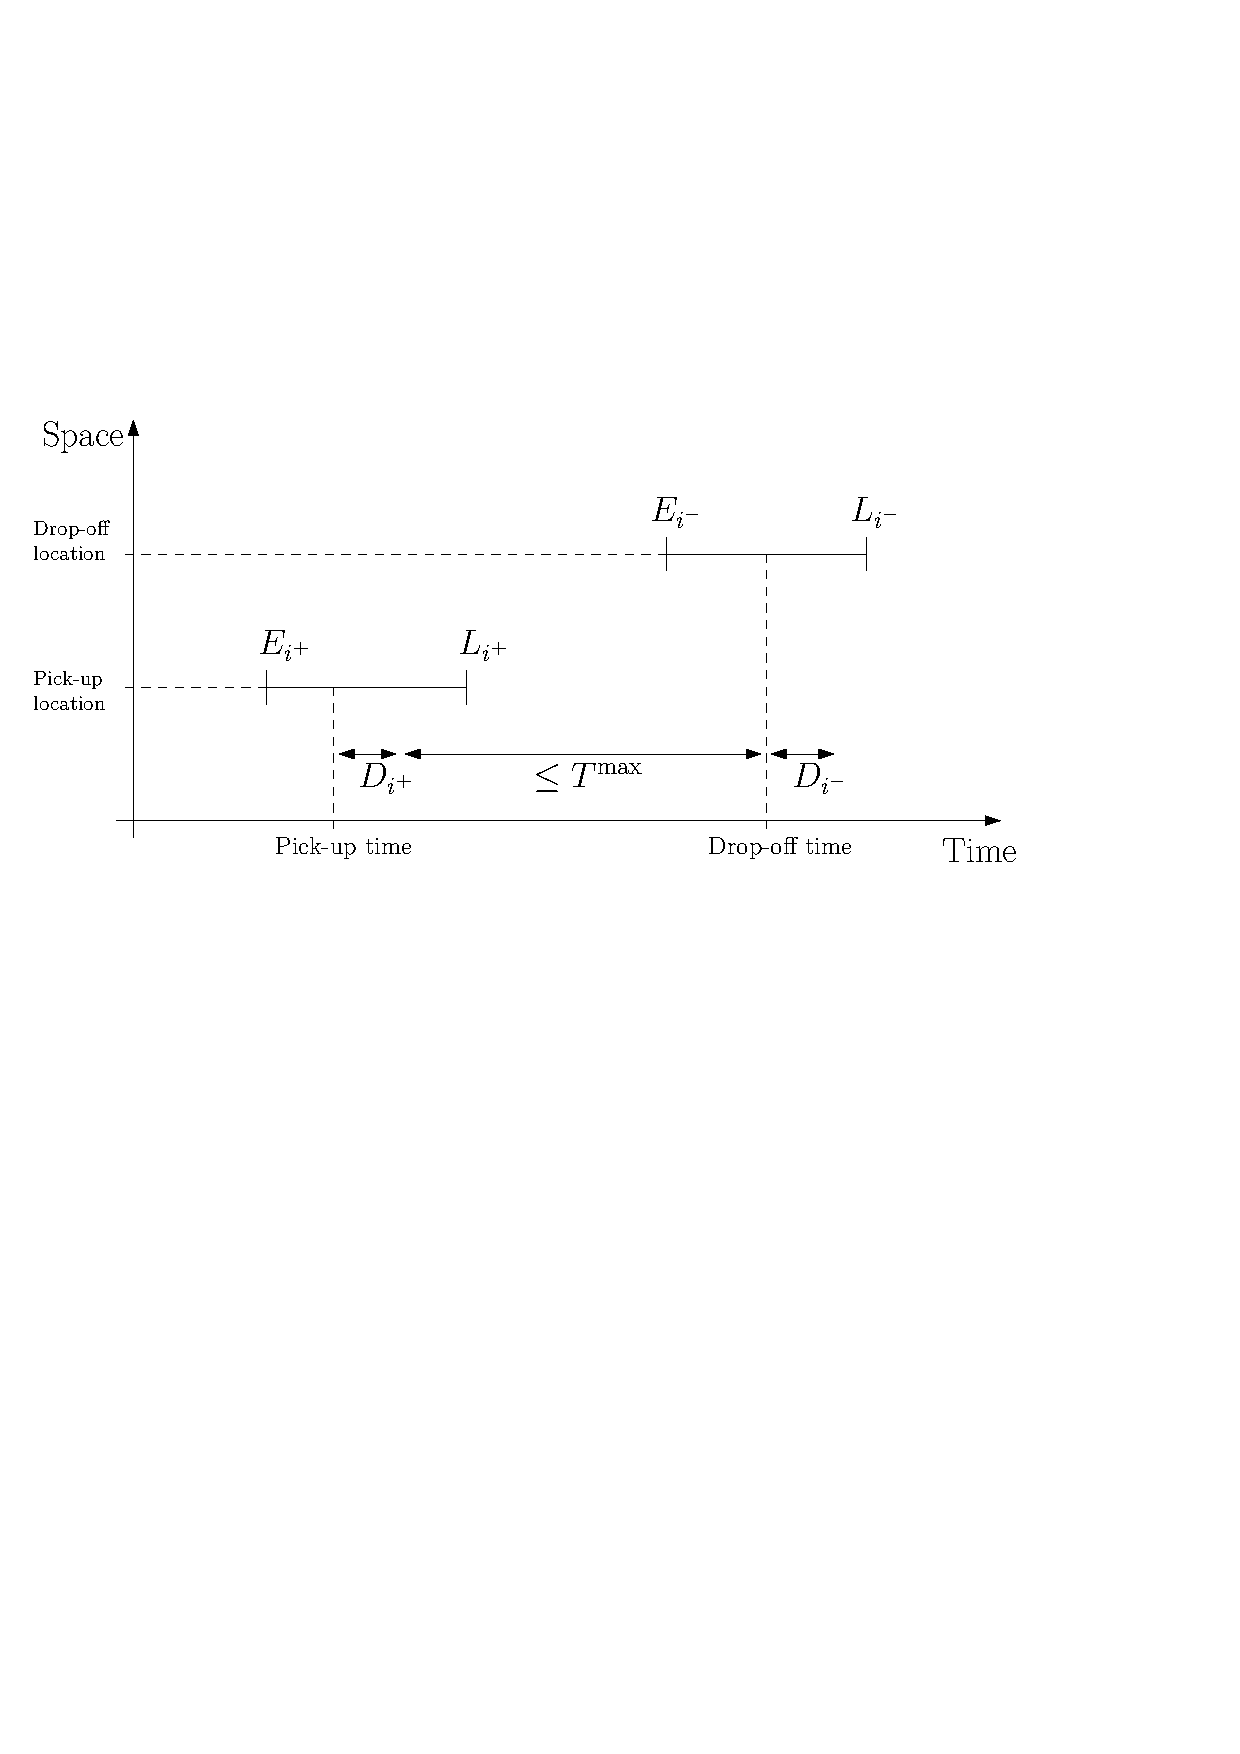
\includegraphics[width=0.8 \columnwidth]{timeline01}
\caption{Pick-up and drop-off time windows. The pick-up point of
customer $i$ is denoted by $i^{+}$ and the drop-off point is denoted by $i^{-}$.
The customer should be picked up at $i^{+}$ within the time window $[E_{i^+},L_{i^+}]$
and the customer should be dropped off at $i^{-}$ within the time window $[E_{i^{-}},L_{i^{-}}]$.
The service times needed for the customer to get on the vehicle
and get off the vehicle are denoted by $D_{i^+}$ and $D_{i^-}$. The time between
the drop-off and the pick-up (excluding $D_{i^+}$) should not exceed the maximum ride time $T^{\max}$.
}
\label{timeline01}
\end{center}
\end{figure}


% \subsection{The dynamic case}
% \label{dynamicdarp}
% Let us discuss the extension of the predescribed single-vehicle dial-a-ride problem to 
% the dynamic case, in which new customers are appended to the route in real time.
% Generally, it can be seen that there is no need to compute a new route
% except when a new customer request occurs, a customer does not show up at the agreed pick-up location,
% the vehicle is ahead or behind of schedule or the vehicle has lost its way. 
% 
% A simple example, similar to the one presented in \cite{psaraftis01},
% on the real-time updating of a vehicle route %might operate 
% is shown in figure \ref{dynamicexample02}.
% Initially, customers $1$ and $2$ have been assigned 
% pick-up and delivery points and corresponding time windows. The vehicle located at $A$ follows the
% tentative optimal route $(1^{+},2^{+},1^{-},2^{-})$,
% where "$+$"-symbols denote pick-up nodes and "$-$"-symbols denote delivery nodes. 
% (see figure \ref{dynamicexample02}a).
% At the time the vehicle is at $B$, the vehicle route is updated with respect 
% to customers $1,2$ and $3$. At this instant %in time, %the procedure revises the
% % nonexecuted portion of the route and produces the 
% a new tentative optimal route shown in figure \ref{dynamicexample02}b is produced. 
% 
% \begin{figure}[ht]
% \begin{center}
% 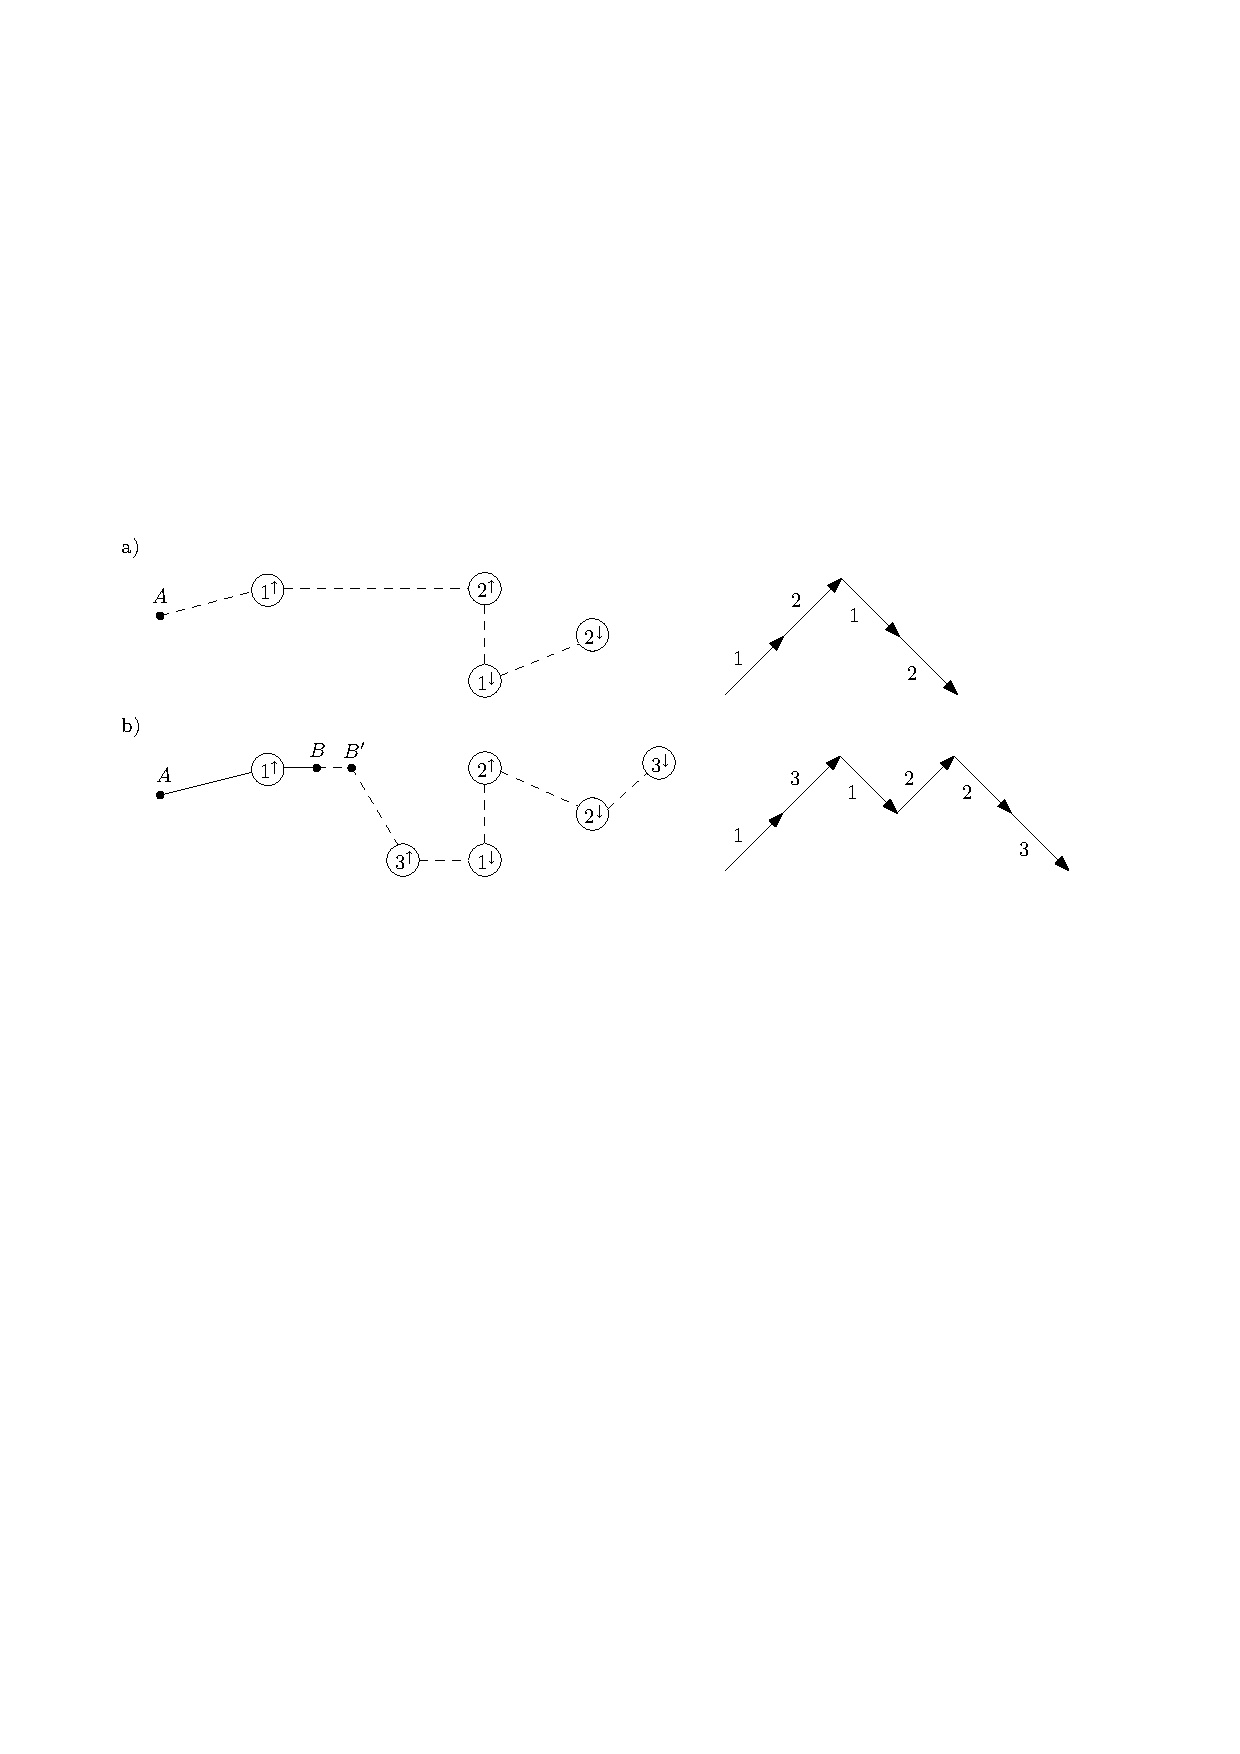
\includegraphics[width=1.0\textwidth]{dynamicexample04.pdf}
% \caption{Modifications in the vehicle route. The route is updated when the vehicle is at $B$ and 
% a new tentative optimal route beginning at $B'$ is produced. 
% The figures on the right show the routes as so-called labeled Dyck 
% paths \cite{cori}, in which each pick-up $i^{+}$ precedes the correspoding drop-off $i^{-}$. 
% At the time a new customer is added to the route, a new path is formed. Clearly, the "height" of the path
% shows the number of customers aboard in different parts of the route.}
% \label{dynamicexample02}
% \end{center}
% \end{figure}
% 
% Note that the new route does not have $B$ as origin, but
% a point $B'$, slightly ahead of $B$. This is due to two facts:
% i) It will take some time for the algorithm to process the new input and reoptimize, 
% ii) It will take some time for the driver
% of the vehicle to process the information regarding the new route. 
% The distance between $B$ and $B'$ depends in general on the particular 
% dial-a-ride service examined. For example, in a highly dynamic setting,
% in which the modification of the route is not
% allowed to take more than a few seconds, it may be assumed that
% the latter of the facts is more restrictive. 
% Any dynamic dial-a-ride
% service should make use of a mechanism to update the point $B'$
% and estimated time of arrival $T'$ at $B'$ at sufficient time intervals.
% The \emph{vehicle checkpoint} $(B',T')$ acts as the starting point for all service sequences.
% 
% 	In addition, for customers that have already been picked up, the pick-up point 
% 	is not a part of the input of the problem. Thus, for such customers
% 	only the delivery point is considered.
% 
% 	In dynamic models, the objective function
% 	used to find the solution over a rolling horizon has often little to do with
% 	the measures developed to evaluate the overall quality of a solution \cite{powell95}.
% 	Generally, the choice of the objective function depends 
% 	on the particular version of the dynamic routing problem and the performance
% 	of different objective functions may be sensitive to, for example, constraints, demand intensity
% 	or the number of vehicles. For a study related to choosing an objetive function
% 	for the immediate-request DARP, the reader is referred to \cite{Hyytia2010}.


\subsection{Adaptive insertion algorithm [\citepub{jeadarp}]}
In general, exact procedures for solving routing  
problems are computationally very demanding, since the complexity is always more or 
less equal to the classical traveling salesman problem.
In addition, exact optimization can be seen to be needless at run-time if routes are modified often. 
Despite these facts, exact algorithms are useful in the sense that the 
performance of different heuristics may be compared to the optimal solution. 

The main idea in the adaptive algorithm presented in \citepub{jeadarp} is that customers are added to 
the vehicle route one by one by using an \emph{exhaustive insertion} method,
which leads to a globally optimal solution, that is, a vehicle route 
which is feasible with respect to all customers and minimizes a given cost function. 

Many studies related to the dial-a-ride problem, see for example \cite{jaw,madsen,diana,wong},
make use of what is called the insertion procedure, in the classical version of which   
the pick-up and delivery node of a new customer are inserted into the 
\emph{current optimal sequence} of pick-up and delivery nodes of existing customers.
%In these references, several improvements to the insertion algorithm 
%have been suggested. However, 
%The main idea of 
That is, the classical insertion algorithm does not take into account the fact that %possibility that the appearance 
the insertion of a new customer may render
the optimal sequencing of existing customers no longer optimal.
%While the basic insertion algorithm can be seen to
%produce relatively good results for unconstrained problems, 
%the performance decreases as the constraints are tightened.

The main idea in the \emph{adaptive insertion algorithm} is to construct the optimal route iteratively by implementing 
an insertion algorithm for each customer, one by one \emph{for all feasible sequences 
of pick-up and delivery nodes of existing customers}.
Namely, the procedure involves two steps for each customer:
%\begin{enumerate}
%	\item 
\\
\\
\noindent 1.	Perform insertion of the new customer to all feasible service sequences with respect to
	existing customers.
%	\item

\noindent 2.	Determine the set of feasible service sequences with respect to the new customer and existing customers.
%\end{enumerate}
\\

It can be readily shown that the insertion of a new customer to all feasible service sequences with respect to 
existing customers 
produces all feasible service sequences with respect to the union of existing customers 
and the new customer and leads to a globally optimal solution but is computationally expensive
if the number of feasible service sequences grows large. However, if the route is constructed under relatively narrow time window constraints,
the number of feasible routes with respect to all customers
will be small compared to the number of all legitimate routes. 
Furthermore, the algorithm is easily extended to an adjustable heuristic algorithm
capable of handling any types of time windows. 

The idea of the advanced insertion method is 
clarified by the following example, where no
capacity or time constraints are taken into account. 

\noindent \textbf{Example.}
Let $i^{+}$ denote the \emph{pick-up node} of customer $i$ and let $i^{-}$ denote 
the \emph{delivery node} of customer $i$.
A \emph{service sequence} is defined as an ordered list consisting of pick-up and delivery nodes.
For instance, the service sequence $( i^{+},  j^{+}, j^{-}, i^{-})$ indicates the order
in which customers $i$ and $j$ are picked up and dropped off.

Let us start the advanced insertion process with customer 1.
Since the pick-up $1^{+}$ of customer 1 has to be before the delivery, $1^{-}$, 
the only possible service sequence at this point is $( 1^{+},  1^{-})$. Thus, the 
set of potential service sequences with respect to customer $1$ consists of this single service sequence. 
By insertion of customer $2$ into the service sequence $( 1^{+}, 1^{-})$ we get the six 
service sequences presented in Table \ref{ykskakstaulukko01}.

By inserting the pick-up and delivery node of customer $3$ into all of these service sequences we get a total
of $6(5+4+3+2+1) = 90$ new potential service sequences. However, if the time and capacity
constraints are taken into account, not all service sequences described above are necessarily feasible.
\\ \
\\ \
\\

\begin{table}[ht] 
\caption{Potential service sequences with respect to customers 1 and 2. 
No capacity or time constraints are taken into account. 
$i^{+}$ denotes the pick-up node and $i^{-}$ denotes
the delivery node of customer $i$.} 
\centering     
\begin{tabular}{|rrrrrr|rrrrrr|rrrrr|}  
\hline  %& & & & & & & & & & & &  & & & &  \\ %[-0.7em]                
A: & $ 1^{+} $ & $  1^{-} $ & $  2^{+} $ & $  2^{-} $ & & 
B: & $ 1^{+} $ & $  2^{+} $ & $  1^{-} $ & $  2^{-} $ & & 
C: & $ 1^{+} $ & $  2^{+} $ & $  2^{-} $ & $  1^{-} $ \\ %[1ex]
\hline  %& & & & & & & & & & & &  & & & &  \\ %[-0.7em]
D: & $ 2^{+} $ & $  1^{+} $ & $  1^{-} $ & $  2^{-} $ & & 
E: & $ 2^{+} $ & $  1^{+} $ & $ 2^{-} $ & $  1^{-} $ & & 
F: & $ 2^{+} $ & $  2^{-} $ & $  1^{+} $ & $  1^{-} $ \\ %[1ex] 
\hline                      
\end{tabular} 
\label{ykskakstaulukko01} 
\end{table} 

% For example, if after the insertion of customer $2$ it can be seen that only the
% service sequences A and B in table \ref{ykskakstaulukko01}, namely 
% $( 1^{+}, 1^{-}, 2^{+}, 2^{-})$ and $( 1^{+}, 2^{+}, 1^{-}, 2^{-})$,
% are feasible with respect to time constraints, then it can be
% shown that all feasible service sequences including customer $3$ are included in
% the sequences given by insertion to these two service sequences, which gives
% a maximum of $2(5+4+3+2+1) = 30$ new potential service sequences.

%Briefly, the structure of the advanced insertion algorithm may be sketched as follows.
%At first, the set of feasible service sequences $S_i$ is determined recursively
%for each customer $i \in \{1, \ldots, N\}$ by inserting the pick-up and delivery nodes of customer $i$ into each feasible
%service sequence with respect to customers $1,\ldots,i-1$. 
In this way the algorithm 
produces the set $S_N$ of all feasible routes with respect to customers $1,\ldots,N$. 
Then the solution to the problem is obtained by choosing the sequence $s \in S_N$ with
minimal cost $C(s)$, where $C(\cdot)$ denotes the cost function, for example, route duration. 

% \subsubsection{Structure and complexity}
% The number of insertions that are tested for feasibility for customer $i$ is bounded above 
% by the formula
% \begin{align}
% n(i) \leq m_{i-1} \sum_{x=1}^{2i-1} x  = \frac{m_{i-1}(2i)(2i-1)}{2},
% \end{align}
% where $m_{i-1}$ is the number of feasible service sequences with respect to customers $1, \ldots,i-1$.
% The inequality can be justified by the fact that not all possible insertions  
% are checked for feasibility. 
% In the worst case, where capacity and time constraints are \emph{not restrictive},
% we get 
% \begin{align*}
% & m_1 = 1, \ \ \ \ \ \ \ m_2 = (4 \cdot 3)/2 = 6,  \ \ \ \ \ \ \ m_3 = 6(6 \cdot 5)/2 = 90, \\
% & m_i = \frac{(2i)(2i-1)}{2} \frac{(2(i-1))(2(i-2)-1)}{2} \cdots \frac{4 \cdot 3}{2} = \frac{(2i)!}{2^i}. 
% \end{align*}
% Thus the maximum number of insertions required in the solution of the static case is
% $\sum_{i=1}^{N}\frac{(2i)!}{2^i} \approx \sum_{i=1}^{N} {2^{1-i} i^{2i + \frac 12} \sqrt{\pi}}$.
% Thus, in the worst case, the number of feasible solutions is of order
% $\mathcal{O}(\sqrt{N} (N^2/2)^N)$.
In the worst case, the number of feasible solutions is of order $\mathcal{O}(\sqrt{N} (N^2/2)^N)$.
However, an average case study of the exact algorithm discussed in Section \ref{svexperience} suggests 
that as time limits reduce the number of feasible solutions, instances with up to 20 customers 
can be solved up to optimality with reasonable computational effort.
In addition, the 
algorithm has a special property of being extendable to an adjustable heuristic,
as described in the following section.

\subsubsection{A heuristic extension}
\label{svheuristic}
Even if the capacity and time constraints were not highly restrictive, the algorithm can be 
modified easily by bounding the size of the set $S_i$ 
of service sequences, in which new customers are inserted, 
by including only a maximum of $L$ service sequences
for each customer $i$. More precisely, if after inserting 
customer $i$, the number of feasible service sequences with respect to customers $1,\ldots, i$
is larger than $L$, the set of feasible service sequences $S_i$ with respect to 
customers $1,\ldots, i$ is narrowed by including only $L$  
service sequences that seem to allow the insertion of remaining customers.
After the last customer has been inserted, the feasible service sequences are evaluated
by means of the objective function.

This modification leads to a heuristic algorithm, in which the computational
effort can be controlled by the parameter $L$, referred to as the \emph{degree} of
the heuristic. The resulting algorithm is
somewhat sophisticated in a way that it produces globally optimal solutions for
small sets of customers. When the number of customers is increased, the
algorithm still produces locally optimal solutions with 
reasonable computational effort. In the special case where $L=1$, the
algorithm reduces to the classical insertion algorithm. 
If $L \geq \frac{(2N)!}{2^N}$, the heuristic coincides with the exact version of the 
algorithm as no routes are discarded.

\subsubsection{Objective functions}
\label{hobjfunc}
In order to be able to efficiently make use of the above heuristic extension
idea, the set of service sequences is narrowed by means of a certain heuristic objective function
after the insertion of each customer.
Since the main purpose of heuristics at the operational level is to always produce some implementable 
solutions very quickly, even if they were only locally optimal, such an objective function should 
be defined in a way that the algorithm is 
capable of producing \emph{feasible} solutions even if the complexity of the problem was high. %was highly constrained.

Looking only at the cost may eliminate from consideration
sequences that are marginally costlier but would easily allow the
insertion of remaining customers in the route. 
Thus, more sophisticated criteria should be considered to help ensure that the heuristic will
find a feasible solution when one exists.

\begin{figure}[ht]
\begin{center}
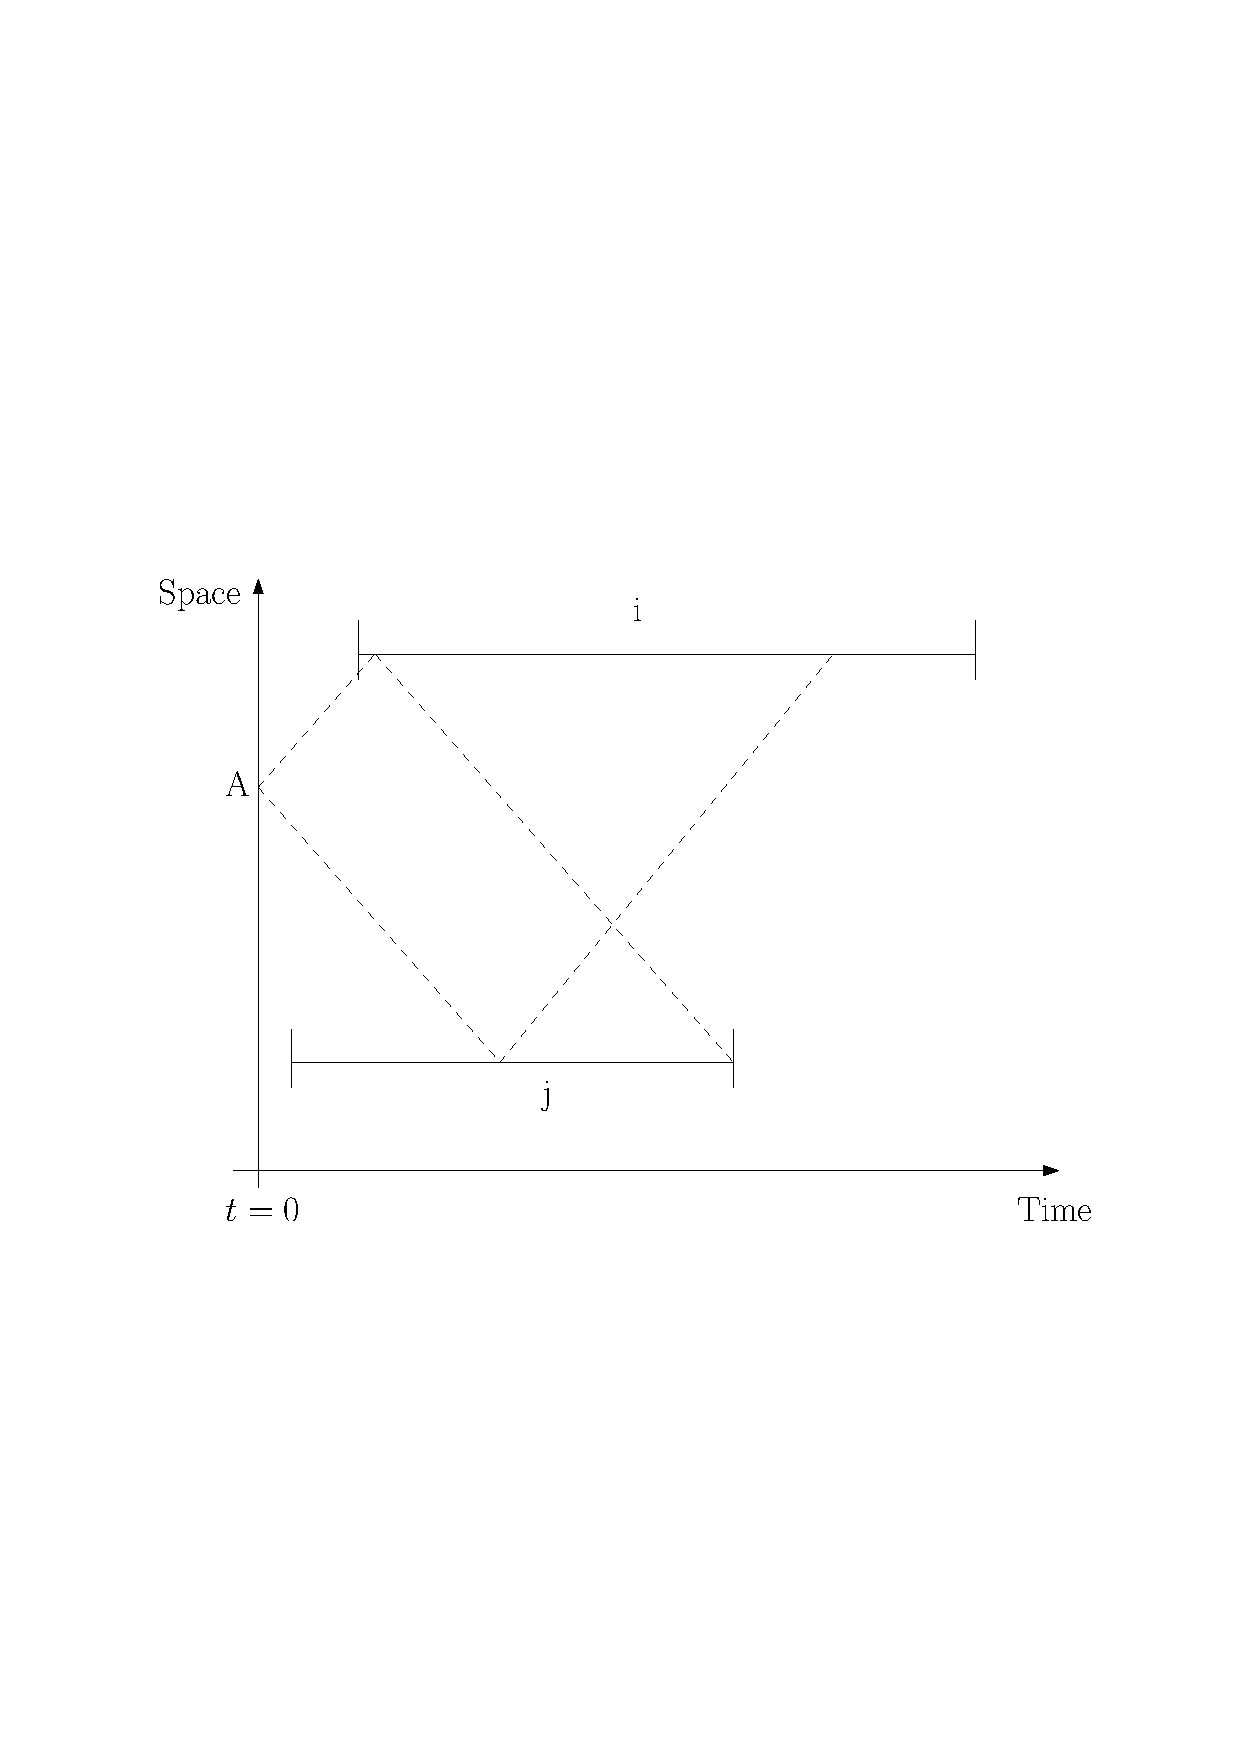
\includegraphics[width=0.7\textwidth]{flexibility03.pdf}
\caption{Route flexibility. A vehicle is located at $A$ at $t = 0$,
and two customers are due to be picked up within the presented time windows at $i$ and $j$.
The dashed lines represent two possible routes for the vehicle.
If the route duration were minimized, $i$ should be visited before $j$. However, since
there would be no "slack time" at $j$, this decision would a priori 
exclude the possibility that new customers could be inserted between $i$ and $j$. 
On the other hand, if $j$ were visited before $i$, there would be
more possibilities for inserting new customers on the route before $i$. }
\label{flexibility01}
\end{center}
\end{figure}


In other words, the function should favor service sequences with enough 
\emph{time slack} for those customers, that have not been inserted into the sequences (see Figure \ref{flexibility01}).
\ref{jeadarp} suggests the following heuristic objectives.

% Given the service sequence $s = (p_1, \ldots, p_{m})$, we wish to optimize one 
% of the functions 
% \begin{align}
% \label{rl}
% f_{rl}(s) &= t_m, & \mbox{(Route duration)} \\
% \label{ts}
% f_{ts}(s) & = \sum_{j=1}^{m} L_j -t_j ,  & \mbox{(Total time slack)} \\
% \label{maxmin}
% f_{min}(s) &= \min_{j \in \{1, \ldots, m\}}  L_j - t_j, & \mbox{(Max-min time slack)} 
% %\label{lastnode}
% %f_{LN}(s) &= L_m - t_m, & \mbox{(Last node time slack)} 
% \end{align}
% where $[E_j,L_j]$ is the time window and $t_j$ is the calculated time of arrival at node $p_j$.
% 
% In general, each of the above objective functions aim to 
% maximize the temporal flexibility of service sequences in different ways.




%\begin{description}
\emph{Route duration}
%The route duration objective function 
favors service sequences in
which the time to serve all customers is as small as possible. 
This objective can be justified by the fact that 
it is likely that new customers may be inserted at the rear of 
a route that is executed quickly.

\emph{Total time slack} 
stores sequences in which
the sum of excess times (or the average excess time) at the nodes is maximized, that
is, sequences which are likely to allow the insertion of a new customer %can be inserted
before the last node.

\emph{Max-min time slack} seeks sequences in which the 
minimum excess time at the nodes of the route is maximized. In other words,
the sequences in which there is at least some time slack at each node
are considered potential.
%\end{description}








\subsection{Routing by ranking [\citepub{jrbrorl}]}
\label{routingbyranking}
Several web information retrieval (IR) methods have been developed
for finding the most appropriate web pages corresponding to 
queries given to search engines. The most sophisticated methods, such as HITS \cite{kleinberg}, PageRank \cite{brin01} and SALSA \cite{lempel}
in use today make use of the hyperlinked structure of the web, since
the goodness of a web page and the position of the page with respect to
other web pages seem to have a certain connection. 
For example, a web page may be
considered good if there are many other web pages linking to that page. In other words, 
web pages are ranked by search engines not only by means of the content of the page, but
also by exploiting information regarding the hyperlink-induced relationships between pages.

The bringing of hyperlinks to bear on the ordering of web pages has given rise to
a mathematical analysis related to hyperlink-induced web IR methods, such as in
\cite{farahat, langville, ng, agosti}, in which the 
behaviour of several IR methods is studied from the computational point of view.

The HITS (Hyperlink-Induced Topic Search) algorithm defines \emph{authorities} 
(web pages with several inlinks) and \emph{hubs} (several outlinks). 
The HITS thesis is that \emph{good hubs point to good authorities and good authorities
are pointed to by good hubs}. Based on this thesis, both a hub score and an authority score is assigned to
each web page \cite{langville}. 

\ref{jrbrorl} presents an application of HITS on the dial-a-ride problem (DARP)
\cite{berbegliathesis,berbegliahybrid,berbegliafeas}.
Here the DARP is examined as a \emph{constraint satisfaction problem}, in which the goal
is to find a feasible vehicle route that serves all customers, or to maximize the number of served customers.



In the context of the dial-a-ride problem, 
the links between nodes are defined as feasible transitions with respect to the %time, capacity and precedence 
constraints of the problem: If node $j$ can be visited after $i$, a link from $i$ to $j$ 
is formed. Thus, a good hub score of a pick-up or drop-off node $i$ means 
that many nodes can be reached in time from $i$. 
Thus, in order to efficiently find feasible solutions to the dial-a-ride problem, we suggest that nodes with large 
hub scores should be visited first since there are many nodes that can
be visited after such nodes. 


\subsubsection{The HITS algorithm \cite{kleinberg}}
\label{hits}
Given a web graph $G = (V,A)$ consisting of pages $V$ and links $A$ between pages,
the authority and hub scores $a_i$ and $h_i$ are computed for each page $i$ as follows.
Letting 
$(i,j)$ represent a link from page $i$ to page $j$, given that each page has been 
assigned an initial authority score $a_i(0)$ and hub score $h_i(0)$, HITS successively
refines these scores by computing
\begin{align*}
a_i(k)  = \sum_{(j,i) \in A} h_j(k-1), \ \ \ \ \ \ \ \ \ \ \  \ \ \ \ \ \ 
h_i(k)  = \sum_{(i,j) \in A} a_j(k-1)
\end{align*}
for $k \in \{1,2,\ldots\}$. By using matrix notation, these equations can be written the form 
$a(k) = L^T h(k-1)$ and $h(k) = L a(k-1)$,
where $a(k)$ is the authority vector containing the authority scores of
each of the pages at step $k$, $h(k)$ is the corresponding hub vector and
$L$ is the adjacency matrix of the graph with elements $L_{ij} = 1$ if
$(i,j) \in A$ and $L=0$ otherwise \cite{langville}. 

It has been shown in \cite{farahat} that the authority and hub vectors
describing the authority and hub scores of nodes of a given graph in the limit are given by 
the dominant eigenvectors of the matrices $L^TL$ and $LL^T$ 
(or equivalently, dominant singular vectors of $L$), 
where $L$ is the adjacency matrix of the graph. 
%Thus the authority and hub
%scores may be efficiently calculated by using eigenvalue (or singular value) algorithms. 

\subsubsection{Modified HITS}
\label{modifiedhits}
For constrained routing problems, a modified version of the HITS algorithm is used, in which only the hub scores
are considered. More precisely, the thesis is that \emph{good hubs point to good hubs}. 
This formulation is motivated by Theorem \ref{polut} below, which states that for a specific class of graphs,
the hub score of a node $i$ corresponds to the number of self-avoiding paths
from $i$ to a given destination node.
When attempting to construct a path that visits all nodes, or to maximize the number of visited nodes, 
the modified HITS idea induces the following intuitive policy: 
Good hubs are visited first, since many nodes can be reached from good hubs. 

The hub scores are calculated as follows.
Let $L$ denote the adjacency matrix of a directed graph $G$. 
Similarly as in the HITS algorithm, the hub vector containing the \emph{hub scores} of nodes is first initialized, $h(0) = (1,1,\ldots,1)$ 
and the hub vector is successively updated by means of the power method
\begin{align}
\label{modhub}
h'(k) & = L h(k-1).
\end{align}
Similarly as in the original HITS algorithm, the hub vector
converges to a dominant eigenvector of $L$.

Theorem \ref{polut} characterizes the hub scores produced by the modified HITS algorithm for 
\emph{sink graphs} defined as follows.
\begin{definition}
\label{sinkg}
Let $G=(V,A)$ be a directed acyclic graph and let $s \in V$ be a node such that $(s,i) \notin A$ for all $i \in V$.
The graph $G_s=(V, A \cup (s,s))$ is called a \emph{sink graph}. 
\end{definition}
In other words, a sink graph is a directed acyclic graph $(V,A)$ with the exception that one node $s \in V$ with zero outdegree is
associated with a loop $(s,s)$.

\begin{theorem}
\label{polut}
Let $L$ denote the adjacency matrix of a sink graph $G_s=(V,A)$, where $V=\{1,\ldots,|V|\}$,  
let $h_i$ denote the number of self-avoiding paths from $i$ to $s$ for $i \in V \setminus \{s\}$ and let $h_s=1$. 
Then, $h=(h_1,\ldots,h_{|V|})^T$ is a unique dominant eigenvector of $L$.
\end{theorem}

Note that since $h_i \geq h_j$ for all $i,j \in V$ for which $L_{ij} = 1$, the vector $h$ defines a \emph{topological
ordering} \cite{cormen} of the nodes for which $h_i > 0$.
% Although Theorem \ref{polut} considers a special class of 
% graphs\footnote{The calculation of self-avoiding paths in graphs with cycles is discussed in \cite{ponstein}.}, 
The result gives us an idea of the behaviour of the modified HITS method: There are many paths beginning from 
nodes with high hub scores. 

In the following section, we show how the 
hub scores are used to guide 
a backtracking algorithm for the dial-a-ride problem.

\subsubsection{The ranking method}
\label{svsolution}
\ref{jrbrorl} presents an exact constraint programming method for the single-vehicle DARP that 
produces a feasible solution whenever one exists or proves that the problem is infeasible.
In the latter case, the algorithm returns a route that maximizes the number of served customers.
% The main challenge is to find a sequence of pick-up and drop-off nodes for which 
% the time and precedence constraints are satisfied. While capacity constraints are 
% also considered, the focus is on problems, in which time limits are more restrictive.

Letting node $0 \in V$ be the location of the vehicle at $t=0$,
we aim to find a feasible path $(0,p_1,\ldots,p_{2n},0)$
consisting of the pick-up and drop-off nodes of $n$ customers.
The number of permutations is $(2n)!$ and the number of feasible permutations
with respect to precedence constraints is $(2n)!/2^n$.

Briefly, the approach to the problem is a \emph{depth-first} search, in which the
remaining nodes are ranked by means of hub scores at each step and the order of the depth-first search is determined by the 
ranking. %\footnote{This idea is remotely similar to lexicographic depth first search (LDFS) \cite{golumbic}.}.
The search begins from node $0$ by ranking the pick-up and drop-off nodes $P$ of all customers.
Then, the node $p^{*}$ with the highest ranking is added to the sequence and the ranking procedure is
repeated for the remaining nodes $P \setminus \{p^{*}\}$.

More formally, at each recursion step, we have the current sequence $S$ 
and the set of remaining nodes $R_S$ (nodes that can possibly be added to the sequence). 
Then, the remaining nodes $R_S$ are ranked by hub scores.
The recursion continues for all sequences $(S,i)$, where $i \in R_S$ in ranked order.
In the following, we describe the ranking of remaining nodes in more detail.


\subsubsection{Hub scores}
\label{feasibility}
The ranking of the remaining nodes $R_S$ is determined in two phases: 
First, the adjacency matrix of the remaining nodes is determined by studying 
\emph{feasible transitions} between the nodes.
Then, the hub vector is calculated by means of Equation \eqref{modhub}.

The definition of feasible transitions is similar to the one studied in \cite{dumas03}, 
in which the set of \emph{admissible arcs} between the pick-up and delivery nodes is constructed
as a preprocessing step in the pickup and delivery problem. The set of admissible arcs is 
made up of arcs which a priori satisfy the precedence, capacity and time constraints of the problem.
The difference in \ref{jrbrorl} is that the feasibility of 
transitions is defined as a function of the state of the vehicle (see Figure \ref{transitions01}).

\begin{figure}[ht]
\begin{center}
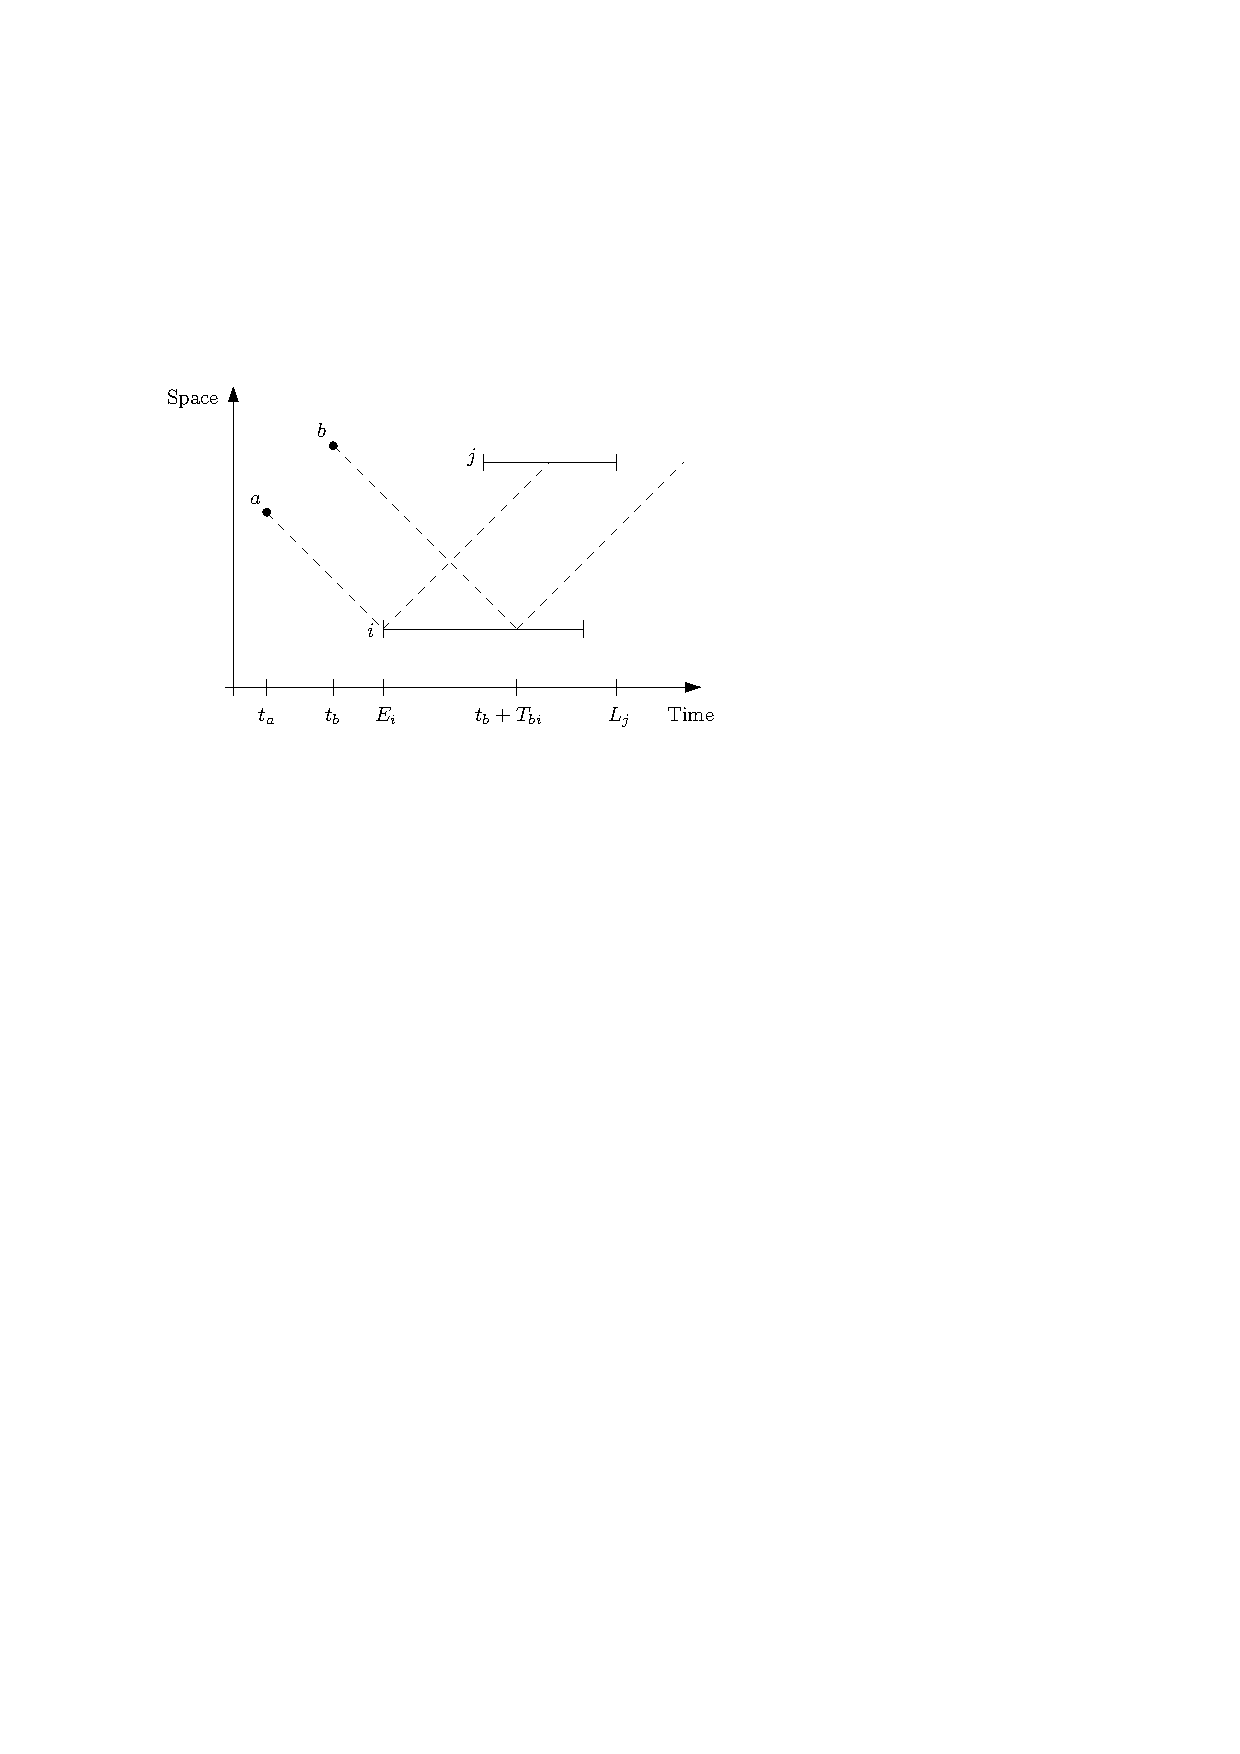
\includegraphics[width=0.7\columnwidth]{transitions01.pdf}
\caption{Feasible transitions. The figure shows the 
locations and time windows of two nodes $i$ and $j$.
If the vehicle left from $a$ at the instant $t_a$, visited node $i$
and moved directly to node $j$, the time constraint $L_j$ would be satisfied. 
However, assuming that at the instant $t_b$ the vehicle is located at $b$, the
transition $i \to j$ is seen to be $S$-infeasible.
}
\label{transitions01}
\end{center}
\end{figure}
The elements of the adjacency matrix are defined for all $i,j \in R_S$ by 
$L_{ij}= 1$, if $i \neq j$ and $i \to j$ is $S$-feasible, $L_{ij} = 0$ otherwise.

After the adjacency matrix $L$ has been determined, the hub vector $h=(h_1,\ldots,h_{|R_S|})$ of $L$ is determined by 
Equation \eqref{modhub} (here the remaining nodes $i \in R_S$ are numbered from $1$ to $|R_S|$ for clarity). 
A large hub score of node $i$ means that many 
nodes can be visited after $i$. 
The hub ranking method is defined as follows.
\begin{definition}[Hub ranking]
The remaining nodes $i \in R_S$ are sorted in descending order of the hub scores $h_i$: 
The branches are evaluated in the order $i_1,\ldots,i_{|R_S|}$, where
$h_{i_1} \geq h_{i_2} \geq \ldots \geq h_{i_{|R_S|}}$.
%branches beginning from good hubs
%are evaluated first.  
\end{definition}

% \textbf{Authority ranking:}
% The remaining nodes are sorted in ascending order of the authority scores; branches beginning from
% bad authorities are evaluated first.
The hub scores are used to give guidance to the algorithm regarding the order in which the 
depth-first search visits the nodes. In the best case, no infeasible states are encountered and thus 
the complexity is of order $\mathcal{O}(n^3)$.

\subsubsection{A heuristic extension}
\label{rrheuristic}
%Section ??? describes an exact procedure for maximizing the number of served customers
%in a single route. In order to find the exact solution, the algorithm goes through all
%branches until no further nodes can be added to the current sequence or the sequence is seen to be suboptimal.
The effort of the algorithm can be controlled by limiting the number of branches that are evaluated
by means of a positive parameter $J$. For example, if $J=1$, the algorithm constructs a single sequence
and stops when the set of remaining nodes is empty. By increasing $J$ the search space is expanded and
if $J = (2n)!/2^n$ (the number of permutations that satisfy precedence constraints), the heuristic
coincides with the exact algorithm.


% \subsubsection{Structure and complexity}
% \label{rrstructure}
% The structure of the ranking algorithm is as follows. 
% Briefly described, each recursion step involves checking the the feasibility
% of sequences $(S,i,j)$, where $i,j \in R_S$.
% Clearly, this process has a complexity of order $\mathcal{O} (|R_S|^2)$,
% where $|R_S|$ is the number of remaining nodes. 
% After the adjacency matrix $L$ of the remaining nodes has been determined, the complexity of 
% calculating $k$ steps of the power method (Equation \eqref{modhub}) is of order $\mathcal{O} (k |R_S|^2)$.
% 
% The overall complexity of finding a feasible solution is strongly dependent on the number of recursion
% steps needed to find the solution. 
% Finding a feasible solution to a problem with $n$ customers involves at least $2n$
% recursion steps: At first, the number of remaining nodes is $2n$ and each time 
% a feasible node is added to the end of the service sequence, the 
% number of remaining nodes is decreased by one.
% In the best case, no infeasible states are encountered and thus there are $2n$ recursion steps 
% (one for each node added to the sequence).
% At step $k \in \{1,\ldots,2n\}$, the number of remaining nodes is $2n+1-k$
% and thus the complexity is of order $\mathcal{O} (\sum_{k=1}^{2n} (2n+1-k)^2) =\mathcal{O}(n^3)$.
% Roughly, the computational work is linearly increased with the 
% number of dead ends $D(n)$ encountered during the recursion.
% The overall complexity of the single vehicle algorithm is thus $\mathcal{O}(D(n)n^3)$.


\subsection{Numerical experiments}
\label{svexperience}
The following paragraphs present a summary of the computational results reported in \ref{jeadarp}. 
The exact and heuristic versions of the single-vehicle advanced insertion algorithm
were tested on a set of problems involving different numbers of customers and different time
window widths determined by a travel time ratio $R$ describing the maximum allowed ratio of travel time
to direct ride time. The pick-up and drop-off points of customers were chosen randomly from a
square-shaped service area and the ride times between the points were modeled by euclidean distances.

At first, the complexity of the problem was studied with respect to three parameters, namely
i) the number of customers $N$, ii) travel time ratio $R$ and iii) the average time interval $\mu$
between customer requests. 
% The complexity was measured in terms of the
% average number of feasible sequences
% in \emph{feasible problem instances}, that is, randomized
% problems for which at least one feasible solution was found. 
% The number of feasible sequences gives us an insight on the complexity of the problem itself,
% since any enumeration algorithm would have to evaluate the same number of feasible sequences.

Then, the performance of the heuristic with different objective functions was evaluated.
The complexity was measured in terms of the number of sequences evaluated by the heuristic.

The experiments were performed on a standard laptop computer with a 2.2 GHz processor. 
The CPU times and the number of evaluated sequences appeared to have a roughly linear relationship.
A typical problem instance involving 20 customers could be solved up to optimality within less than a second.


\subsubsection{Experiment 1: Number of customers}
%At first we study the complexity of the exact algorithm with respect to the number of customers.
% In practice, the number of customers assigned to a single vehicle is governed by the
% pre-order time of the dial-a-ride service: If customers may request service in
% advance, the planned vehicle routes are expected to be longer than in immediate-request
% services. 
Figure \ref{nvertailu01} shows, as a function of the number of customers, the average number of feasible sequences in feasible problem instances 
on a logarithmic scale.
%, computed over 10000
%randomized instances for $N=1\ldots 20$, $R = 2,2.5,3$ and $\mu = 1800$s.

% \begin{figure}[ht]
% \begin{center}
% 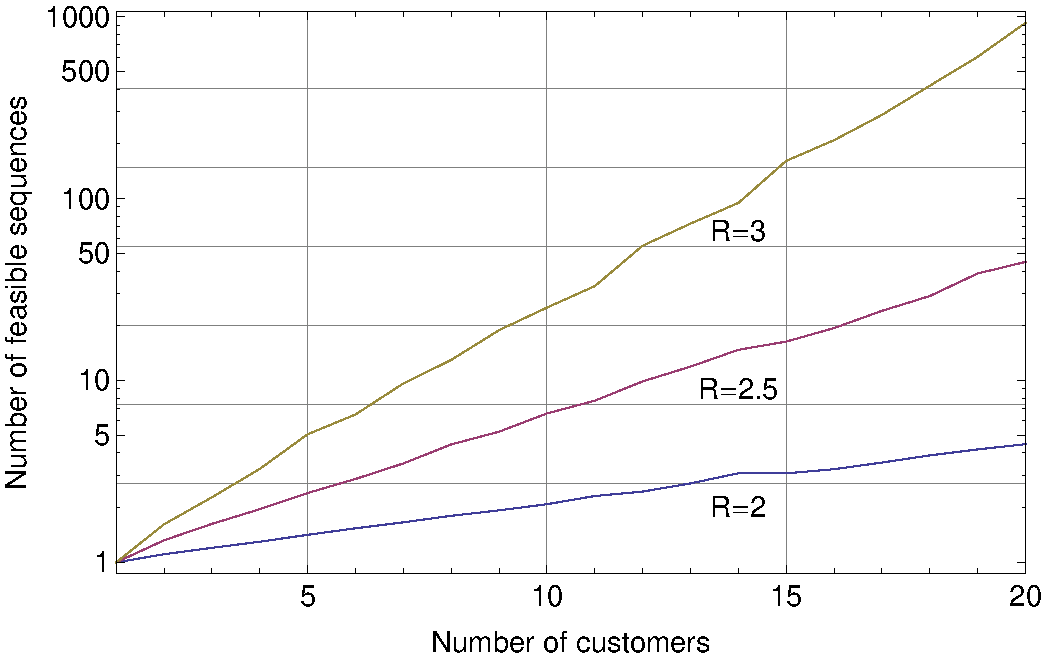
\includegraphics[width=0.7\textwidth]{nvertailu01.pdf}
% \caption{Experiment 1. The complexity of the exact algorithm with respect to the number of customers on a logarithmic scale. 
% The three curves represent, as a function of the number of customers, the average number of feasible sequences 
% for $R=2,2.5,3$ and $\mu=1800$s. Clearly, the complexity increases exponentially with respect
% to the number of customers.}
% \label{nvertailu01}
% \end{center}
% \end{figure}

\begin{figure}
\centering
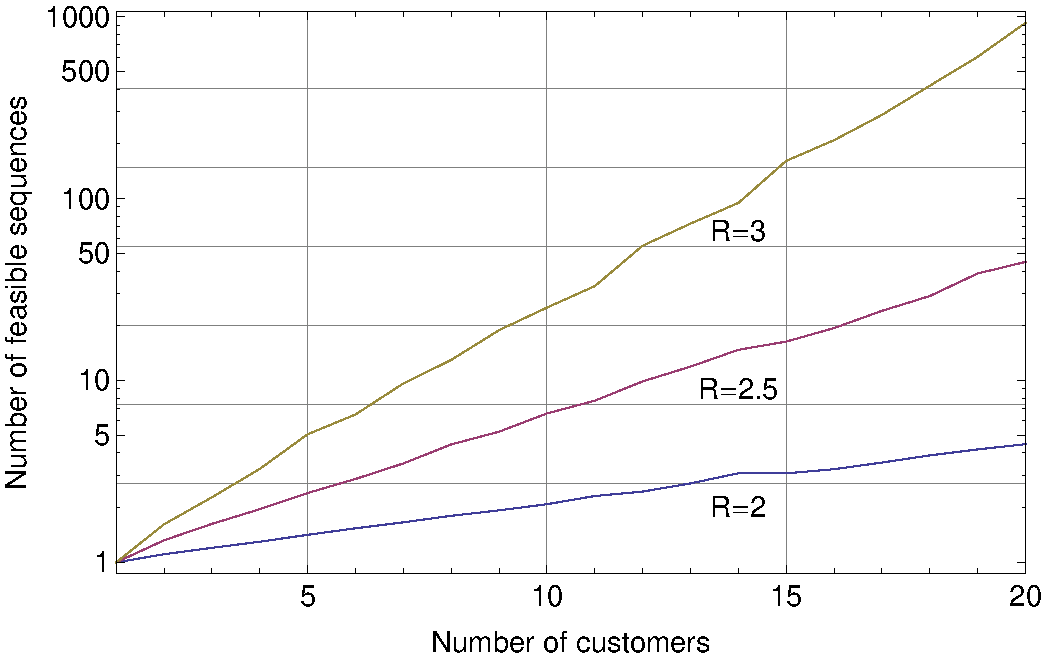
\includegraphics[width=0.7\textwidth]{nvertailu01.pdf}
\caption{Experiment 1. The complexity of the exact algorithm with respect to the number of customers on a logarithmic scale. 
The three curves represent, as a function of the number of customers, the average number of feasible sequences 
for $R=2,2.5,3$ and $\mu=1800$s. }
\label{nvertailu01}
\end{figure}

\begin{figure}
\centering
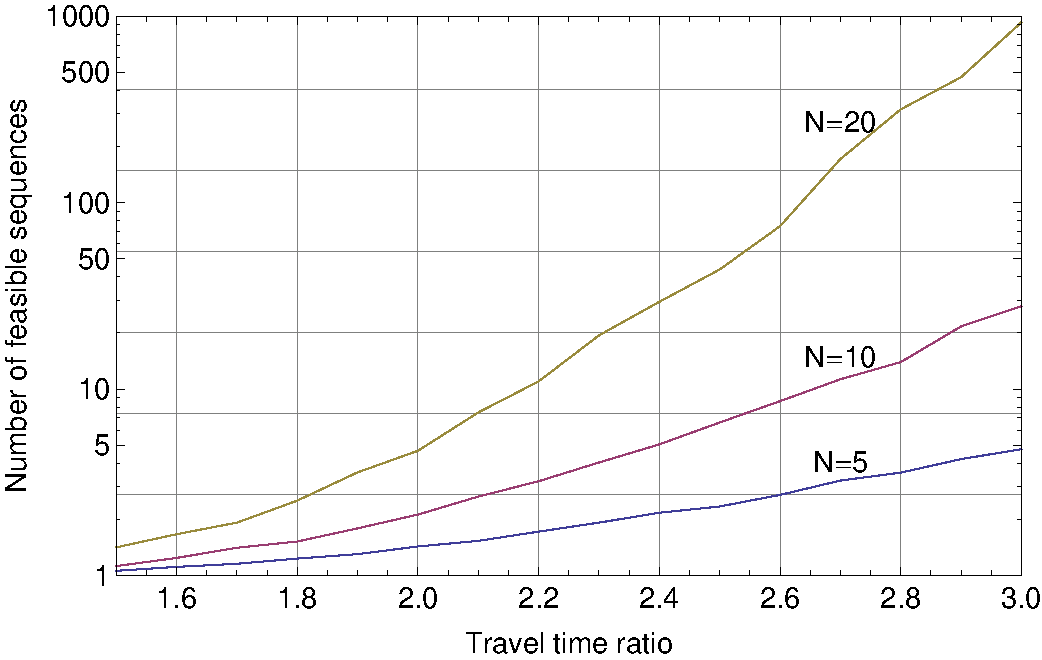
\includegraphics[width=0.7\textwidth]{ttivertailu01.pdf}
\caption{Experiment 2. The complexity of the exact algorithm with respect to travel time ratio on a logarithmic scale. 
The three curves represent, as a function of the travel time ratio, the average number of feasible sequences
for $N=5,10,20$ and $\mu = 1800$s.}
\label{ttivertailu01}
\end{figure}





Referring to the figure, it can be seen that the complexity of the problem increases exponentially
with respect to the number of customers with all studied values of the travel time ratio.  
In addition, the complexity is increased with the travel time ratio. 



\subsubsection{Experiment 2: Travel time ratio}
%Let us study the complexity of the exact algorithm as a function of travel time ratio.
Figure \ref{ttivertailu01} shows, as a function of travel time ratio, the average number of feasible sequences in feasible problem instances 
on a logarithmic scale.
%, computed over 10000
%randomized instances for $R=1.5\ldots 3$, $N = 5,10,20$ and $\mu = 1800$s. 

% \begin{figure}[ht]
% \begin{center}
% 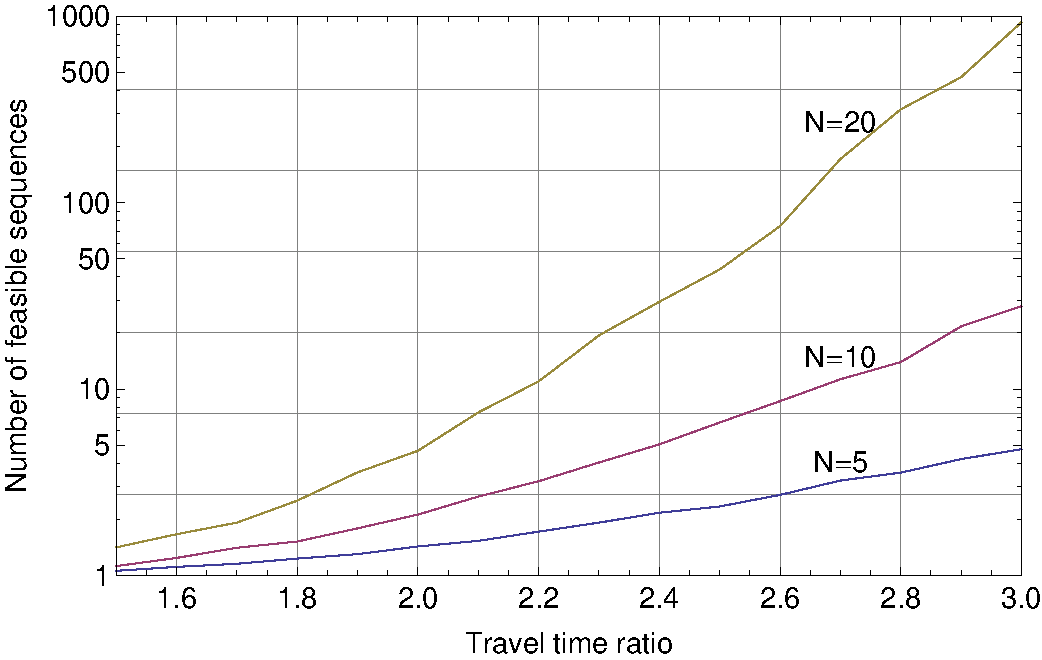
\includegraphics[width=0.7\textwidth]{ttivertailu01.pdf}
% \caption{Experiment 2. The complexity of the exact algorithm with respect to travel time ratio on a logarithmic scale. 
% The three curves represent, as a function of the travel time ratio, the average number of feasible sequences
% for $N=5,10,20$ and $\mu = 1800$s.}
% \label{ttivertailu01}
% \end{center}
% \end{figure}


The figure shows that the effect of the travel time ratio on the complexity of the problem is significant.
The fact that the slopes of the curves increase with $R$ on the logarithmic scale indicates that the relation 
between complexity and $R$ is super-exponential.






\subsubsection{Experiment 3: Time interval}
%Let us conclude the study of the exact algorithm by examining complexity with respect to the average time interval between customer requests. 
The solid lines in Figure \ref{intvertailu01} represent, as a function of average time interval 
between requests, the average number of feasible sequences in
(i) feasible problem instances and (ii) all problem instances, on a logarithmic scale.
%, computed over 10000
%randomized instances for $N=10$, $R=3$ and $\mu = 6 \ldots 40$ minutes. 
The dashed line corresponds to the fraction
of problem instances, for which at least one feasible solution was found.

% \begin{figure}[ht]
% \begin{center}
% \includegraphics[width=0.7\textwidth]{intvertailu01-crop.pdf}
% \caption{Experiment 3. The complexity of the exact algorithm with respect to the average time 
% interval between customers. The solid lines represent the average number of feasible sequences in
% feasible problem instances and all problem instances, on a logarithmic scale for $N=10$ and $R=3$.
% The dashed line corresponds to the fraction
% of problem instances, for which at least one feasible solution was found.}
% \label{intvertailu01}
% \end{center}
% \end{figure}

\begin{figure}
\centering
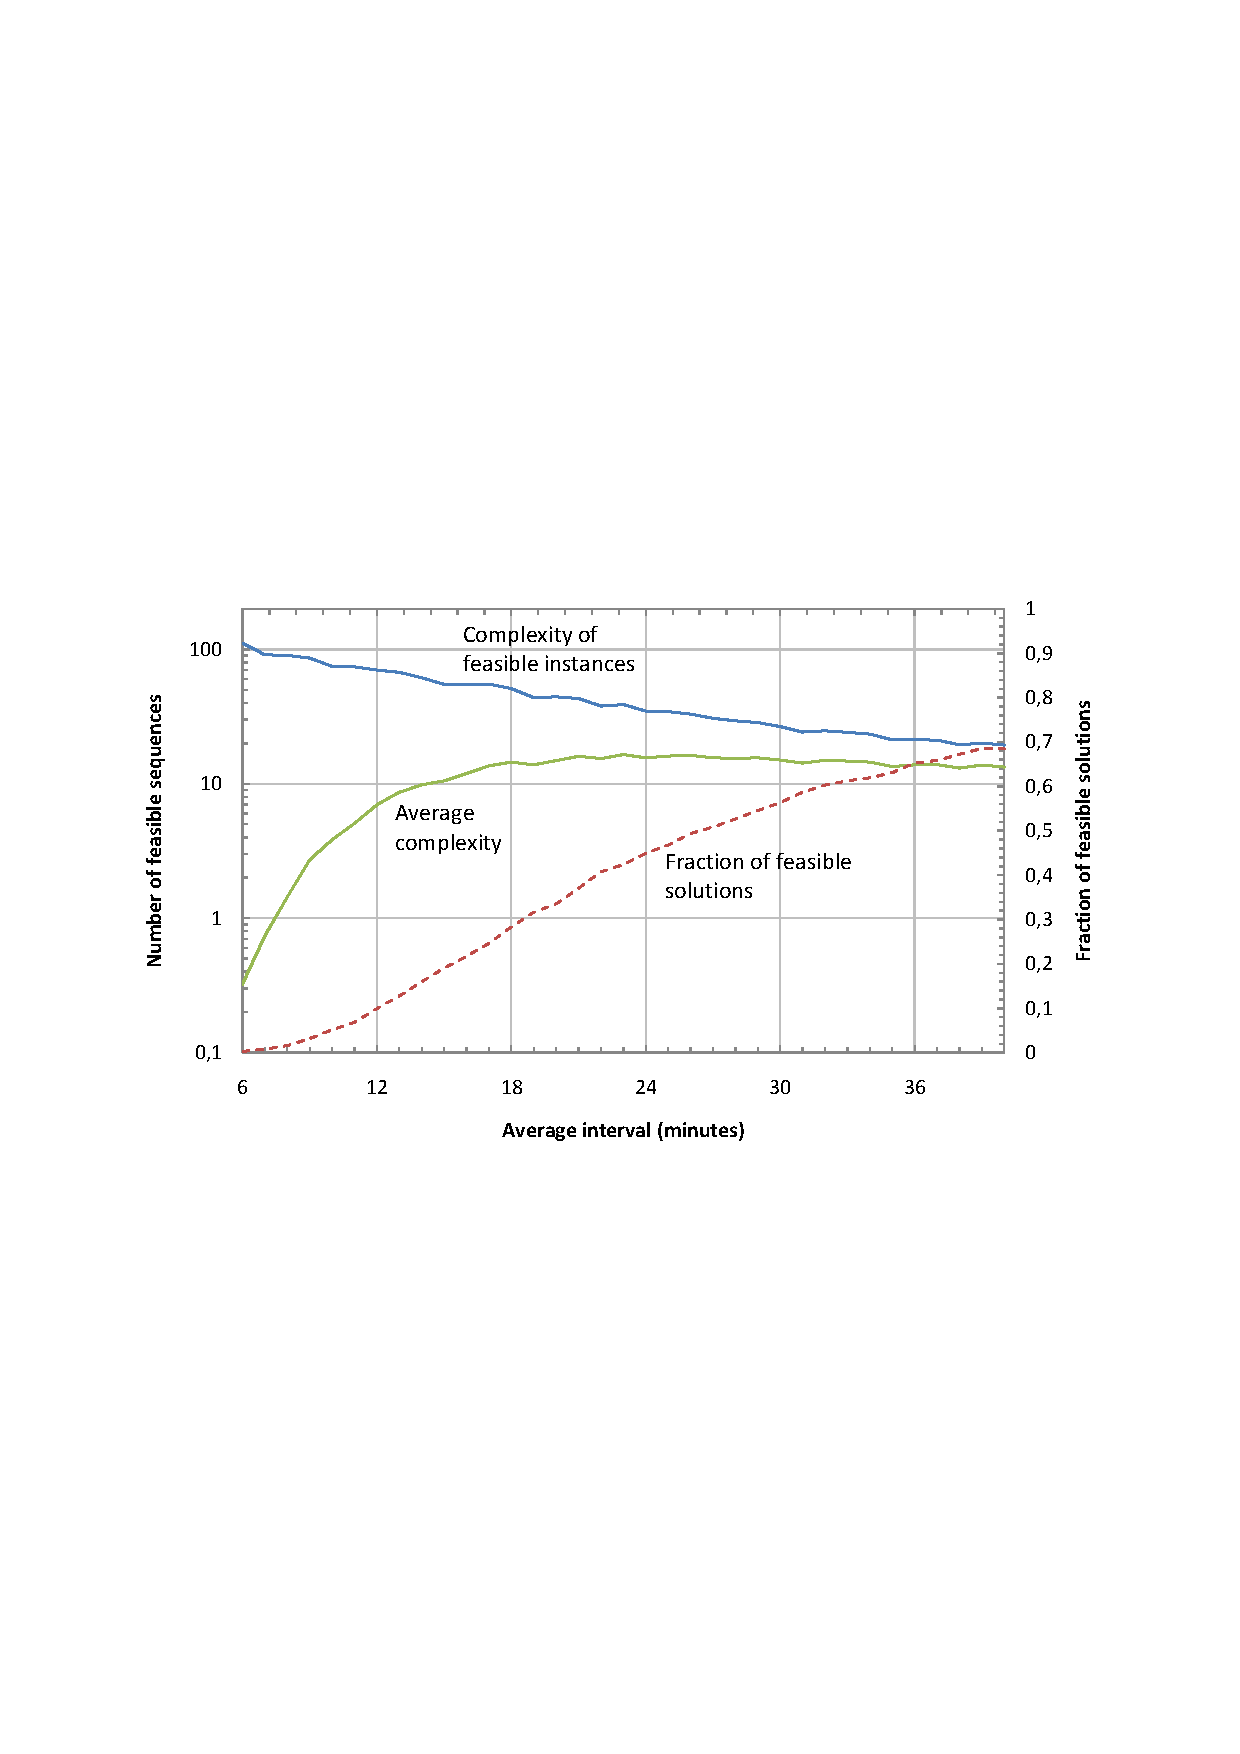
\includegraphics[width=0.7\textwidth]{intvertailu01.pdf}
\caption{Experiment 3. The complexity of the exact algorithm with respect to the average time 
interval between customers. The solid lines represent the average number of feasible sequences in
feasible problem instances and all problem instances, on a logarithmic scale for $N=10$ and $R=3$.
The dashed line corresponds to the fraction
of problem instances, for which at least one feasible solution was found.}
\label{intvertailu01}
\end{figure}



The figure indicates that the complexity of feasible problem instances decreases exponentially 
with respect to the average time interval $\mu$. On the other hand, the probability of finding
at least one feasible solution is increased with $\mu$. By looking at the curve corresponding 
to the average complexity of all problem instances (including infeasible cases), it can be seen that the
complexity is maximized at a certain time interval ($\mu = 24$ minutes in this case), in which both the probability of
finding a feasible solution and the number of feasible sequences in feasible cases are relatively large.

%At this point, it should be emphasized that the above results apply to randomized instances for the 
%single vehicle problem. In a dynamic multiple vehicle setting, an effort is made to 
%divide the customers among available vehicles optimally. Thus, it is suggested that a larger number of customers
%can be served by a single vehicle in less time than in the case in which the customers' pick-up
%and drop-off locations are completely random. However, the above results give us an insight on
%how the complexity of the single vehicle subroutine behaves with respect to the average time interval between
%the earliest pick-up times of customers assigned to a single vehicle.




% \begin{figure}[ht]
% \begin{center}
% 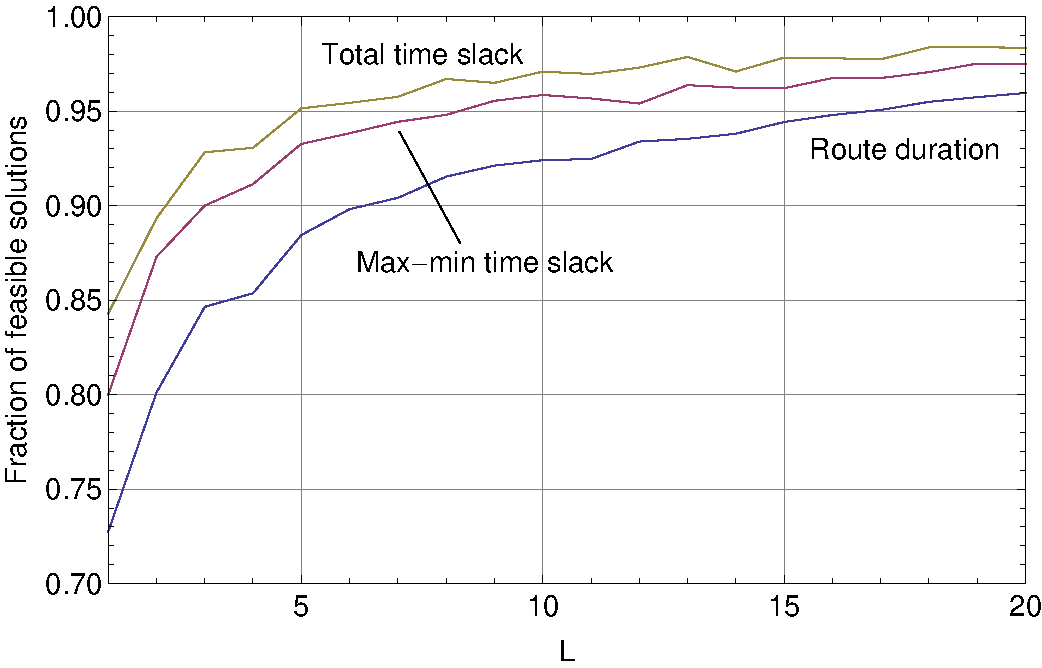
\includegraphics[width=0.7\textwidth]{objvertailu01.pdf}
% \caption{Experiment 4. The performance of three different heuristic objective functions as functions of degree $L$.
% The curves represent the fractions of instances for which a feasible solution was found by the objective functions 
% (compared to the exact algorithm), 
% for $N=20$, $R=3$ and $\mu=1800$s. The total slack time objective function
% outperforms the other two in all studied cases.
% }
% \label{objvertailu01}
% \end{center}
% \end{figure}



\subsubsection{Experiment 4: Objective functions}
Let us study the performance of three different heuristic cost functions %\eqref{rl}, \eqref{ts} and \eqref{maxmin}
as a function of the degree $L$ of the heuristic.
Figure \ref{objvertailu01} shows the fraction of problem instances for which a feasible solution was 
% in feasible problem instances obtained 
found by the heuristic (compared to the exact algorithm). 

%, computed over 10000
%randomized instances. 
%The number of customers was set to $N=20$, the travel time ratio
%was $3$ and the average time interval $\mu = 1800$s was used.

\begin{figure}
\centering
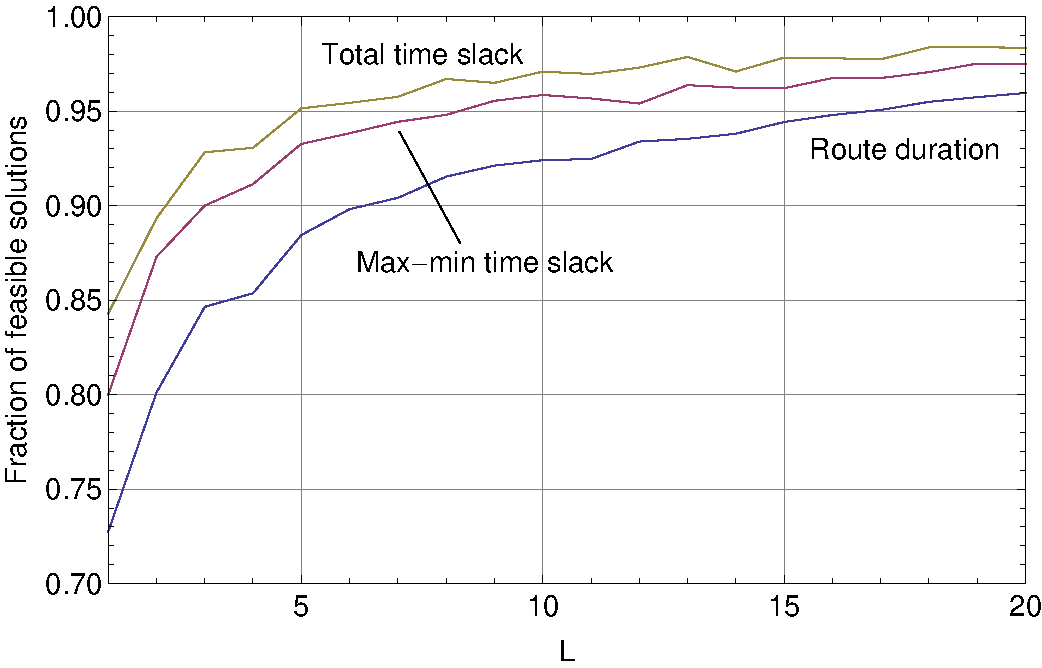
\includegraphics[width=0.7\textwidth]{objvertailu01.pdf}
\caption{Experiment 4. The performance of three different heuristic objective functions as functions of degree $L$.
The curves represent the fractions of instances for which a feasible solution was found by the objective functions 
(compared to the exact algorithm), 
for $N=20$, $R=3$ and $\mu=1800$s. The total slack time objective function
outperforms the other two in all studied cases.
}
\label{objvertailu01}
\end{figure}


Referring to the figure, it can be seen that the total time slack cost function is capable of finding
a feasible solution to randomized problems most often, while the performance of the route duration cost
function is worst of the three algorithms. Note that as the degree $L$ is increased, 
the fraction of feasible solutions converges to 1 for any heuristic cost function, since whenever $L \geq \frac{(2N)!}{2^N}$,
the heuristic coincides with the exact algorithm regardless of the studied problem.



\section{Multi-vehicle dial-a-ride problem}
\label{multivehicle}
Most recent studies related to the dial-a-ride problem are related to the multi-vehicle case, in which 
a set of vehicle routes is designed for a predefined set of customers, see for example 
\cite{cordeau02, cordeau01, bent, ropke, xiang2006, melachrinoudis, parragh, garaix, berbegliathesis,berbegliafeas,berbegliapdp}.
Reference \cite{berbegliafeas} examines the multi-vehicle dial-a-ride problem as a \emph{constraint satisfaction problem}, in which the goal
is to find a set of $m$ feasible vehicle routes that serve all customers, where $m$ is the 
number of vehicles, or to prove that such a set of routes does not exist.
In this reference, it is noted that 
an algorithm for checking the feasibility of a multi-vehicle DARP instance has two main applications:  
1) Determining the feasibility can be the first phase in an 
optimization algorithm in a \emph{static} setting, where all trip requests are known, for example, one day in advance. 
2) In \emph{dynamic} services, a constraint satisfaction algorithm can be used 
for deciding whether to accept or reject incoming user requests. 
% 
% In addition to passenger transportation, we note that a time-constrained problem similar to the DARP arises in 
% food delivery services. Instead of passengers with pick-up and drop-off time windows, the goal is to transport 
% \emph{meals} from restaurants to specified delivery points within guaranteed time limits.
% Similarly as in the dynamic DARP, the food delivery service provider needs to decide quickly whether to take an incoming order or not,
% if there is a guaranteed maximum delivery time, for example, one hour.

% The main result of \ref{jhitsdarpts} is an exact algorithm for the constraint satisfaction dial-a-ride problem
% introduced in \cite{berbegliafeas}. In contrast to most works related to vehicle routing and dial-a-ride problems,
% no specific cost function is considered\footnote{
% For approaches to vehicle routing and dial-a-ride problems with cost functions, 
% see \cite{braysy01,braysy02,groer} and \cite{cordeau02,berbegliahybrid}.}. 
% The algorithm stops as soon as a feasible solution is found regardless of
% the quality of the solution. If a feasible solution is not found through exhaustive search, the algorithm 
% proves that the problem instance is infeasible. In addition, some infeasible instances are detected in advance
% by studying the feasibility of routes involving two customers. 


\subsection{The maximum cluster algorithm [\ref{jhitsdarpts}]}
\label{mvsolution}
\ref{jhitsdarpts} presents the following exact approach to the multi-vehicle DARP as a constraint satisfaction problem.
By using the ranking algorithm  described in Section \ref{routingbyranking} as a subroutine,
 the method produces a feasible solution to 
any instance or proves that the instance is infeasible. The main idea is that the vehicle routes are constructed
one by one, each maximizing the number of served customers in the set of remaining customers.
The customers are denoted by numbers $1,\ldots,n$ and the vehicles are denoted by numbers $1,\ldots,m$.

\begin{figure}[ht]
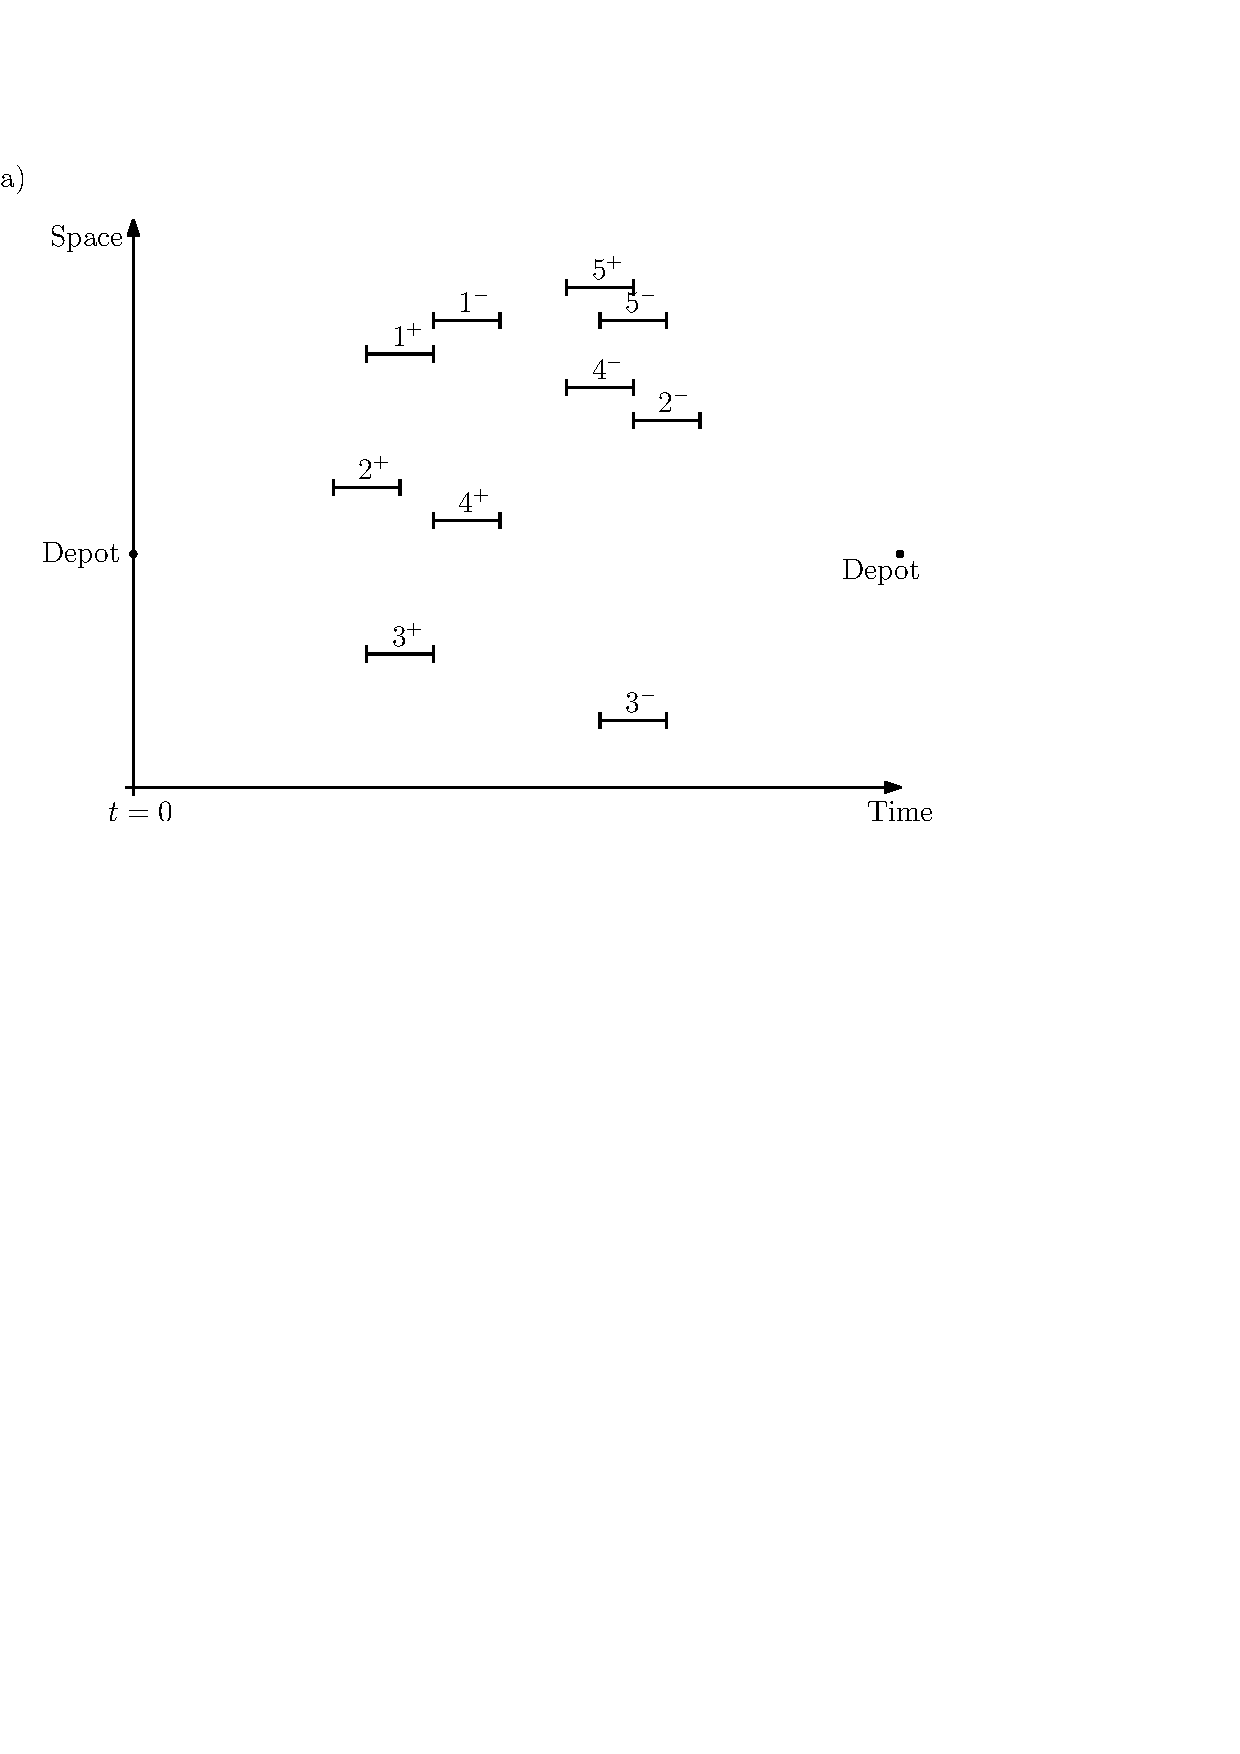
\includegraphics[width=0.5\textwidth]{greedy01b.pdf} \ 
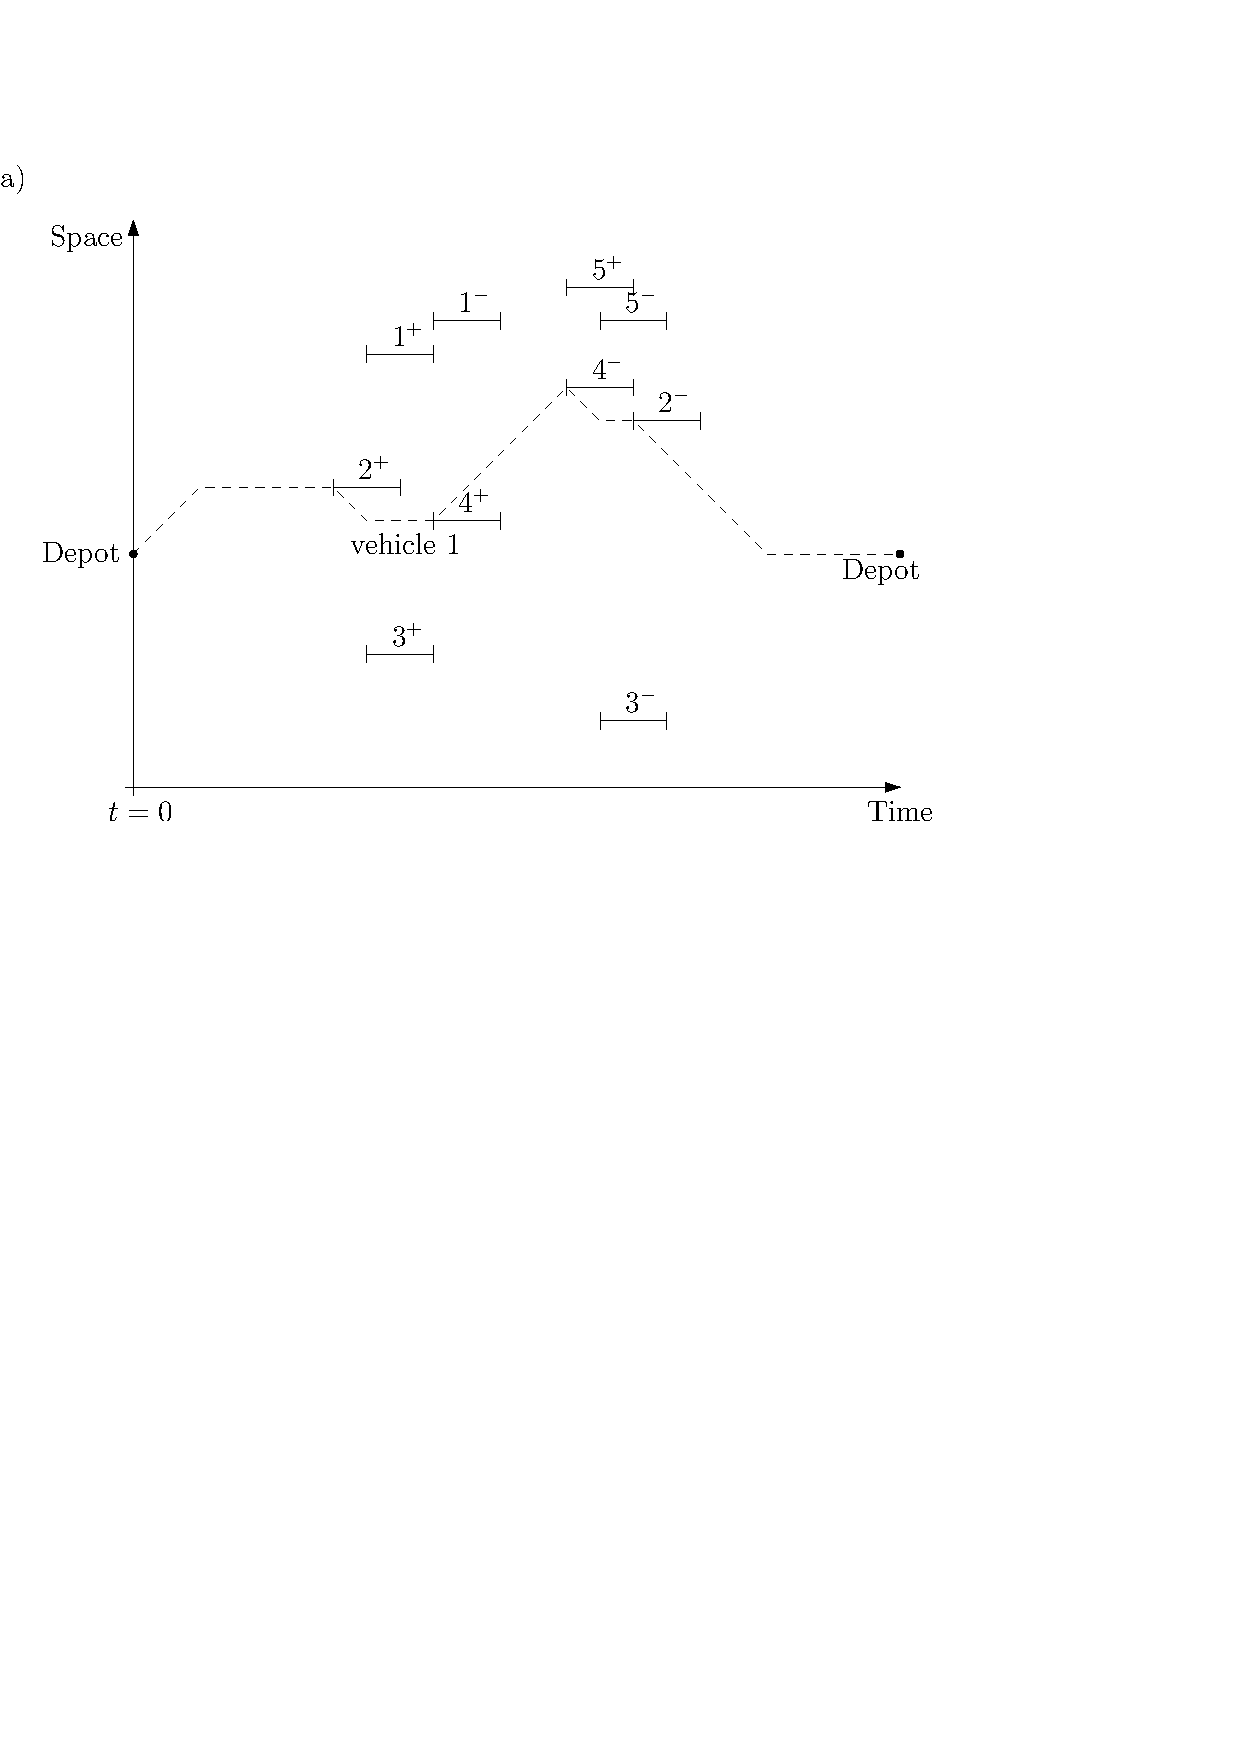
\includegraphics[width=0.5\textwidth]{greedy05b.pdf}  \\ \ \\  
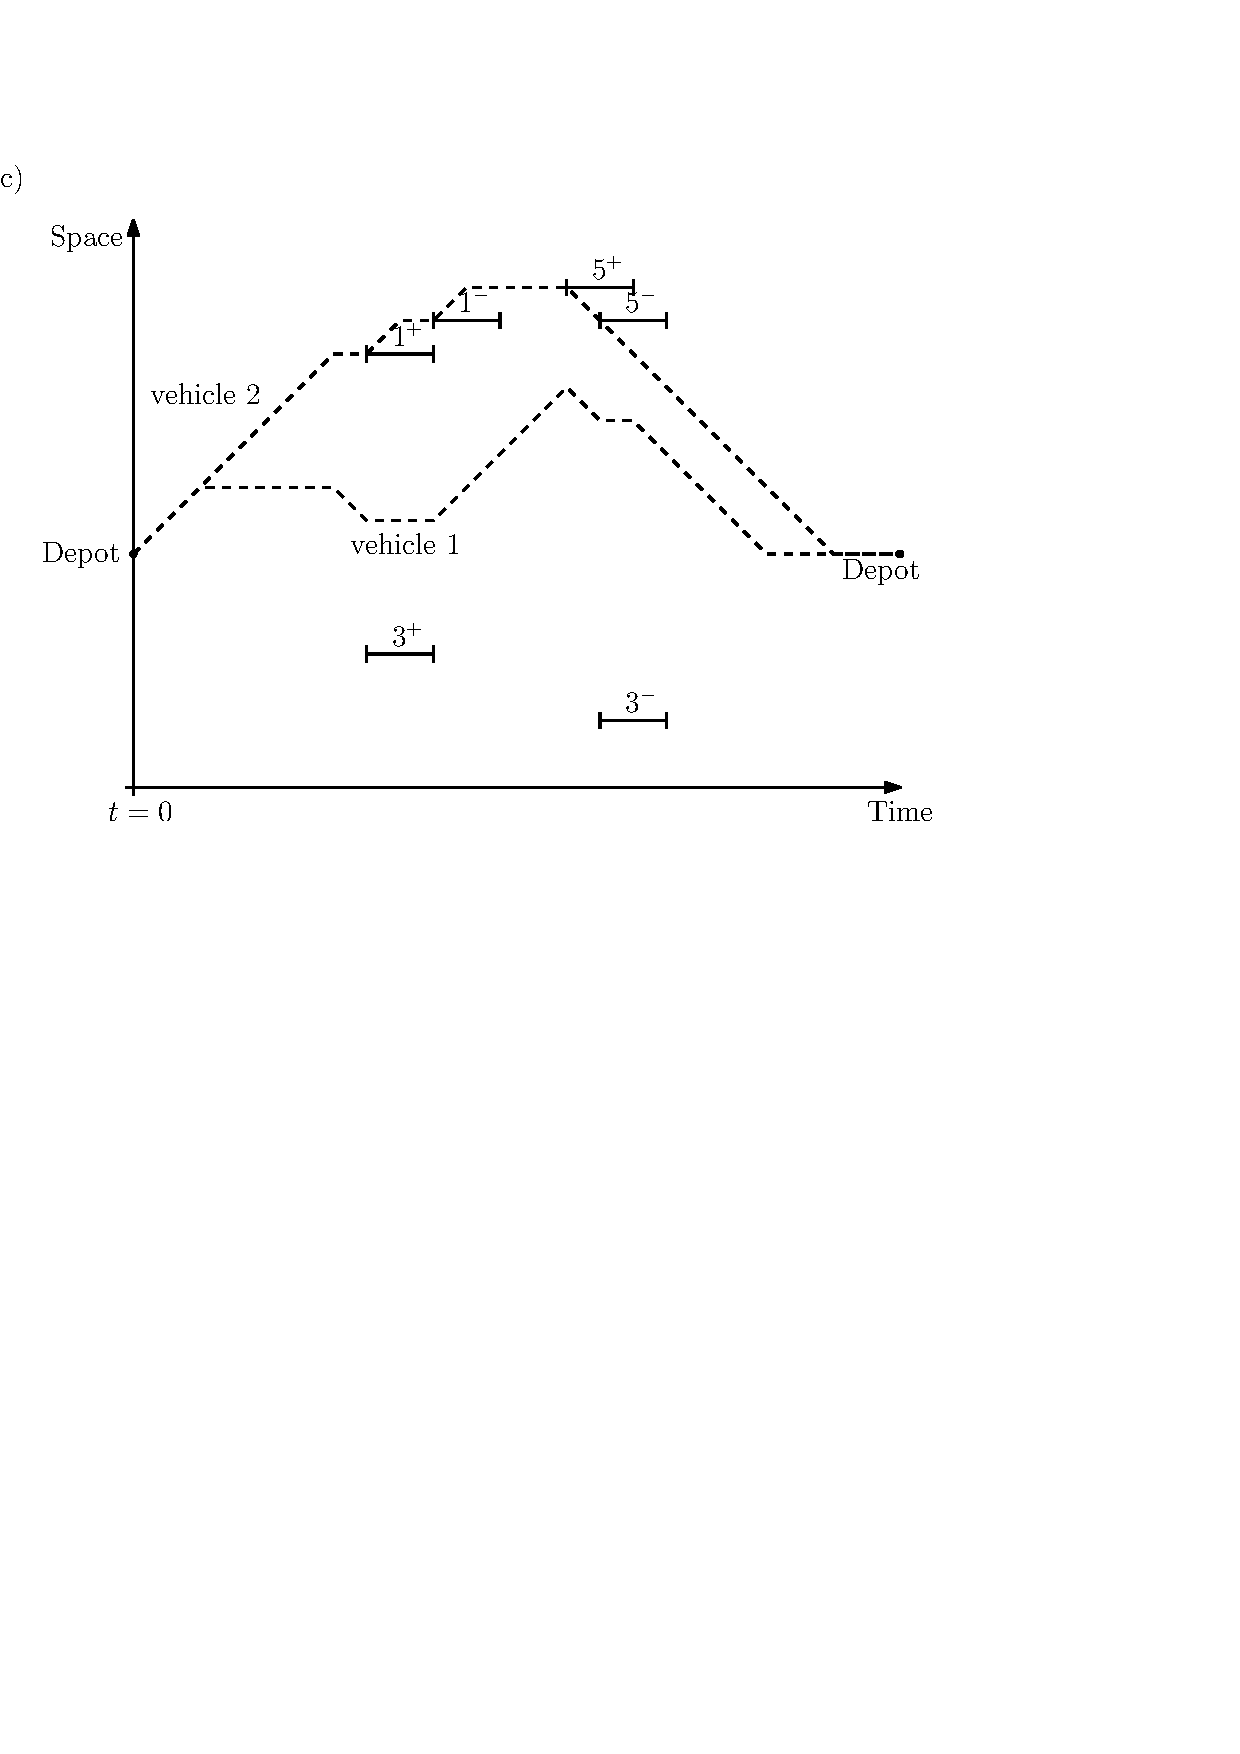
\includegraphics[width=0.5\textwidth]{greedy06b.pdf} \   
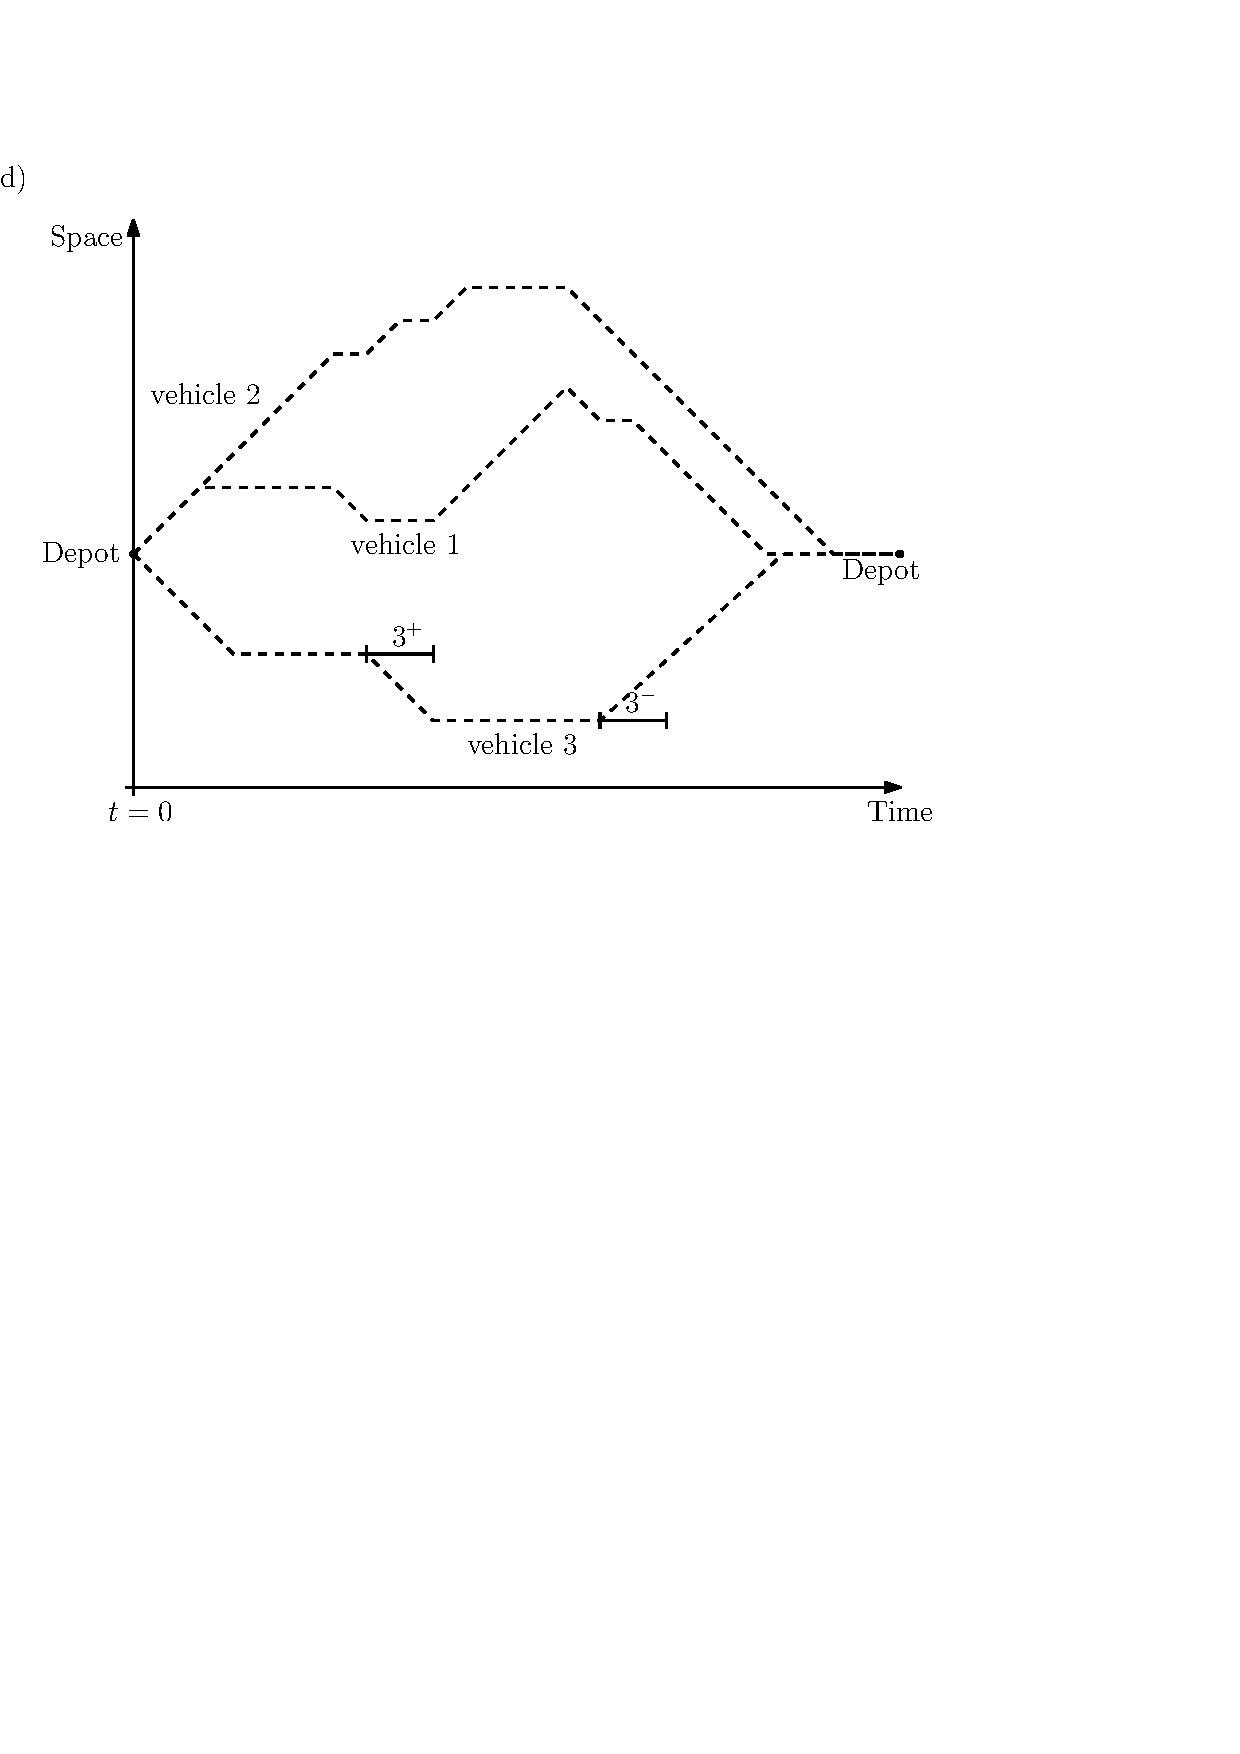
\includegraphics[width=0.5\textwidth]{greedy07b.pdf}  \\ \ \\   
\caption{A one-dimensional example of the approach to the multi-vehicle problem involving five customers 
and three vehicles. The first route is constructed by maximizing 
the number of customers that can be served by a single vehicle (Figure b). 
Then, the customers $2$ and $4$ served by the first vehicle are removed from the set of remaining customers and the process 
is repeated for the second vehicle (Figure c). Finally, a route is constructed for the third vehicle, serving the
last remaining customer $3$ (Figure d).
}
\label{greedyidea}
\end{figure}

First, a route is constructed for vehicle $1$, serving as many 
customers as possible. Then, the process is repeated with vehicle $2$ for the set of customers
that were not served by vehicle $1$ and so forth (see Figure \ref{greedyidea}). 
If a feasible solution is not found directly, % by using the above procedure, %described in Algorithm \ref{alg02}, 
the process is repeated by attempting to add the remaining customers to the existing vehicle routes. 
% Letting $X$ denote a
% set of customers, we denote by SV($X$) a single-vehicle subroutine
% that returns a route 
% that maximizes the number of served customers in set $X$ and the corresponding set of served customers.
% Formally, a \emph{maximum cluster} of a set $X$ of customers is defined as follows.
% 
% \begin{definition}
% \label{maxdef}
% Let $X$ be a set of customers and $M \subset X$ be a subset of $X$, for which there exists a feasible 
% route serving all customers in $M$. If $|M| \geq |Y|$ for all sets $Y \subset X$
% for which there exists a feasible route serving all customers in $Y$, then $M$ is a \emph{maximum cluster} of $X$.
% \end{definition}
% Note that if there exists a feasible route serving all customers in $X$, we have $M(X) = X$.
%Note that such a route always exists, since one can always construct a route in
%which no customers are served. 
%The solution to the multi-vehicle case is outlined in Algorithm \ref{alg02}.

% \begin{algorithm}
% \begin{algorithmic}
% {\footnotesize
% \FORALL {$v \in \{1,\ldots,m\}$}
% \STATE \ \ $[S_v,X_v'] \leftarrow $ SV($X_v$); \ \ \ \ \ ($S_v$ = route, $X_v'$ = set of served customers)
% \STATE \ \ $X_{k+1}  \leftarrow X_{k+1}' \cup (X_v \setminus X_v')$, where $X_{m+1} = X_1$ and $X_{m+1}'=X_1'$;
% \ENDFOR
% }
% \end{algorithmic}
% \caption{Outline of the multi-vehicle algorithm. $X_v$ denotes the set of customers assigned 
% to vehicle $v$ and SV($X_v$) denotes a single-vehicle 
% subroutine (for example Algorithm \ref{alg01}) that returns
% a maximum cluster $X_v'$ of $X_v$ and the corresponding route $S_v$. Initially, all customers are assigned to the first vehicle, 
% that is, $X_1 = \{1,\ldots,n\}$ and $X_v = X_v' = \emptyset$ for all $v \in \{2,\ldots,m\}$.}
% \label{alg02}
% \end{algorithm}

% 
% 
% More precisely, the first iteration starts with the candidate partition
% $(X_1,\ldots,X_m) = (\{1,\ldots,n\},\emptyset,\ldots,\emptyset)$, 
% and produces the sets \\ $X_1', X_2', \ldots, X_m'$ containing the customers that are successfully included in the feasible vehicle routes.
% The following iterations repeat the process for the candidate partition $(X_1,\ldots,X_m) = (X_1' \cup X_R,X_2',\ldots,X_m')$,
% %, the single-vehicle algorithm is first executed for $X_1' \cup X_R$, 
% where $X_R$ denotes the set of customers that were not served by any vehicle during the previous iteration.
% %Letting $X_R'$ denote the set of customers that were not served in $X_1' \cup X_R$, the algorithm proceeds by
% %executing the single-vehicle algorithm for $X_2' \cup X_R'$ and so forth.
% If an iteration results in a visited partition of customers, a non-visited candidate partition is generated.
% If all possible candidate partitions have been checked, the problem is infeasible.

% The iterative process is justified by the fact that a customer $x$ with relatively few out-links to all nodes may 
% be in a good position with respect to the customers assigned to a
% single vehicle $v$. That is, even if customer $x$ was left out of the initial 
% vehicle routes due to a small number of links to other nodes,
% $x$ can be added to one of the routes during a later iteration. 

The above approach produces a set of customer-vehicle assignments 
such that for each vehicle there exists a feasible route serving all customers assigned to the vehicle
or proves infeasibility by going through all possible sets of customer-vehicle assignments.


\subsection{A priori screening}
\label{earlydetection}
Since the  
number of possible partitions of $n$ customers into $m$ sets is equal to the Stirling number of the second kind, that is,
$|\mathcal{P}| = S_2(n,m) = \frac {1}{m!} \sum_{i=0}^{m} (-1)^i {m \choose i} (m-i)^n$,
going through all possible partitions is computationally taxing. However, some instances 
are rendered infeasible by studying routes consisting two customers: 
If all possible routes consisting of customers $\{i,j\}$ are infeasible, an arc between $i$ and $j$ is formed 
(customers $i$ and $j$ can not be assigned to the same vehicle). Then, we find the \emph{maximum clique} $C$
within the set of customers (the largest set for which there is
an arc between all $i,j \in C$). If the size $|C|$ of the maximum clique
is greater than the number $m$ of vehicles, the instance is infeasible.

Otherwise, since the customers in the maximum clique $C = \{c_1,\ldots,c_{|C|}\}$ all have to be assigned to different vehicles, 
with no loss of generality we may initially assign customer $c_j$ to vehicle $j$ for all $j \in \{1,\ldots,|C|\}$.
Then, the set of \emph{feasible vehicles} $V_i$ for each customer $i$ is determined by noting that if there is an 
arc between $i$ and $c_j \in C$, customer $i$ may not be assigned to the same vehicle as $c_j$.

Note that assigning each customer $i$ a vehicle number $v_i \in V_i$ defines a unique partition.
Since the vehicle number of customer $i$ can be chosen from the set $V_i$ of feasible vehicles, 
the number of a priori feasible partitions is given by $|\mathcal{P}'| = \prod_{i=1}^n |V_i|$, which yields the following result.

\begin{theorem}
\label{partitions}
The number of a priori feasible partitions satisfies $|\mathcal{P}'| \leq m^{n-|C|}$.
\end{theorem}


% \subsection{Structure and complexity}
% \label{mvstructure}
% The multi-vehicle algorithm involves solving the single-vehicle case
% for each vehicle in $r$ iterations. Thus the complexity is bounded above by $\mathcal{O}\left(rmD(n)n^3\right)$, 
% where the number of dead ends satisfies $D(n) \leq (2n)!/2^n$.                                                                                                                  
% 
% % Note that the complexity is in general lower since the size of the set of customers is
% % $n$ only for the first vehicle in the first iteration. For the other vehicles, the number of customers is
% % smaller since the customers that are already included in another vehicle route
% % are not a part of the subproblem. 
% Since the total number of possible partitions is 
% equal to the Stirling number of the second kind, the number of iterations $r$ needed to find a feasible solution
% or to prove infeasibility satisfies $r \leq S_2(n,m) = \frac {1}{m!} \sum_{i=0}^{m} (-1)^i {m \choose i} (m-i)^n$.
% Given the maximum clique $C$ (see section \ref{earlydetection}), we have $r \leq |\mathcal{P}'| = \prod_{i=1}^n |V_i| \leq m^{n-|C|}$.

In summary, the worst case complexity is high especially when the set of a priori feasible partitions $\mathcal{P}'$ is large. 
However, as will be seen in the next section, solutions to problems with loose constraints are usually found with little effort. 
On the other hand, tight constraints reduce the set of a priori feasible partitions $\mathcal{P}'$ 
and thus also the complexity of the algorithm.


\subsection{Numerical experiments}
\label{mvexperience}
In the following, an algorithm using the ranking idea is compared with two existing solution methods,
namely, a tabu search algorithm \citep{cordeau02} and
a constraint programming (CP) algorithm \citep{berbegliafeas}. 

The ranking algorithm was implemented in Matlab and the tests were performed on a 2.2 GHz Dual Core Intel PC. 
The tabu and CP algorithms were tested on a 2.5 GHz Dual Core AMD Opteron computer \citep{berbegliathesis}. 

In the studied instances the pick-up and drop-off points are located in a $20 \times 20$ square and the 
ride times between points (in minutes) are equal to Euclidean distances. The time windows
have 15 minutes of length. 
The instances are described in more detail in \citep{cordeau01,ropke2007,berbegliafeas}.

The results of the tests are shown in Table \ref{comparisontable}. The first
column shows the instance labels of the form $am$-$n$ or $bm$-$n$, where $m$
indicates the number of vehicles and $n$ corresponds to the number of customers.
The other columns show the average time (in seconds) needed to solve the
instances and the corresponding modifications by using the different solution methods,
calculated over ten runs. 
% The results obtained by the first two algorithms, tabu and CP, have been reported
% previously in \citep{berbegliathesis,berbegliafeas}\footnote{The computing time for the instance 
% 'b6-48' has been reported for the tabu algorithm in \citep{ropke2007}.}. 
A number in parentheses indicates that the instance was proven to be infeasible,
a dash indicates that a solution was not found in three minutes computing time and
a star indicates that results for the instance have not been reported. 
% First, the heuristic version of the ranking algorithm was executed with $L=1$. If a solution was not found and the problem
% was not rendered infeasible by the a priori screening procedure described in
% Section \ref{earlydetection}, the exact version of the algorithm was executed.

\begin{table}
{\tiny
\begin{center}
\begin{tabular}{|c|ccc|ccc|ccc|ccc|}
\hline
Instance & \multicolumn{3}{|c|}{Original} & \multicolumn{3}{|c|}{RT=30} & \multicolumn{3}{|c|}{RT=22} & \multicolumn{3}{|c|}{75 \% of vehicles} \\
\hline
& Tabu & CP & Ranking & Tabu & CP & Ranking & Tabu & CP & Ranking & Tabu & CP & Ranking\\
\hline
a4-40 & 0.8 & 0.5 & 0.02 & 0.8 & 0.5 & 0.02 &0.5 & 0.3 &0.05 & 1.7 & 0.3 & 0.64\\ % (0.2)\\
\hline
a4-48 & 1.0 & 0.5 & 0.05 & 1.0 & 0.5 & 0.05 &1.3 & 0.4 &0.05& 78.5 & 0.6 & 0.08 \\ % (0.2)\\
\hline
a5-40 & 0.3 & 0.3 & 0.02 & 0.3 & 0.3 & 0.02 &0.3 & 0.3 &0.02& 1.3 & 0.3 & 0.02\\ % 0.2 \\
\hline
a5-50 & 0.7 & 0.5 & 0.04 & 0.7 & 0.5 & 0.04 &0.6 & 0.6 &0.03& 3.9 & 1.3 &2.0\\ % 0.3\\
\hline
a5-60 & 1.4 & 1.0 & 0.05    & 1.4 & 1.0 & 0.05 &1.5 & 0.9 &0.05& - & 24.5 & 64.7 \\ % 0.5 \\
\hline
a6-48 & 0.4 & 0.6 & 0.03    & 0.4 & 0.6 & 0.03 &0.4 & 0.7 &0.03& 1.1 & 0.5 &0.07\\ % 0.2 \\
\hline
a6-60 & 1.0 & 5.6 & 0.04    & 1.0 & 5.6 & 0.04 & - & (1.1) &(0.63)& 11.6 & 6.2 & 10.7 \\ % (0.4)\\
\hline
a6-72 & 1.9 & 5.0 &  0.06   & 1.9 & 5.0 & 0.06 & - & (1.7) &(0.77) & 5.7 & 2.0 &0.90\\ % 0.7\\
\hline
a7-56 & 0.5 & 1.8 &  0.04   & 0.5 & 1.8 & 0.04 & - & (0.6) &(0.40)& 0.9 & 1.5 &0.06\\ % 0.3 \\
\hline
a7-70 & 1.7 & 41.5 & 0.06   & 1.7 & 41.5 & 0.06 & 1.4 & 7.6 &0.06& 3.2 & 5.1 &0.06\\ % 0.6 \\
\hline
a7-84 & 2.7 & 3.4 & 0.08   & 2.7 & 3.4 & 0.08 & 3.0 & 4.1 &0.08& 7.5 & 3.5 &0.07\\ % 1.0\\
\hline
a8-64 & 0.8 & 6.2 & 0.05    & 0.8 & 6.2 & 0.05 & - &  (1.9) & (0.84) & 1.1 & 2.5 &0.04\\ % 0.4\\
\hline
a8-80 & 1.5 & 8.5 & 0.07    & 1.5 & 8.5 & 0.07 & 1.8 & 6.0 &0.07& 3.0 & 3.6 &0.07\\ % 0.9\\
\hline
a8-96 & 3.5 & 37.7 & 0.11   & 3.5 & 38.7 & 0.11 &- & (3.7) & (1.72) & 8.1 & 5.3 &0.15\\ % 1.6 \\
\hline
b4-40 & 0.6 & 0.4 & 0.02    & 0.4 & 0.3 & 0.05 & 0.4 & 0.3 &0.05& - &(0.1) & (0.40) \\ % (0.1)\\
\hline
b4-48 & 1.3 & 0.4 & 0.03    & 1.6 & 0.4 & 0.08 & - & (0.1) & (0.32) & - & (0.1) & (0.59)\\ % (0.2)\\
\hline
b5-40 & 0.4 & 0.3 & 0.03    & 0.4 & 0.4 & 0.03 & - & (0.1) & (0.27) & - &  (0.1) & (0.37)\\ % 0.1\\
\hline
b5-50 & 1.2 & 6.8 & 0.06    & 0.9 & 0.8 & 0.05 & 1.1 & 0.9 &0.18& - & (0.1) & (0.58) \\ % (0.2)\\
\hline
b5-60 & 1.5 & 109.5 & 0.04  & 1.8 & 3.1 & 0.04 & 1.6 & 1.2 &0.04& - & (0.1) & (0.78) \\ % 0.4\\
\hline
b6-48 & 0.3 & * & 0.02    & * & * & 0.02 & * & * &0.02& * & * & (0.54) \\ % 0.3\\
\hline
b6-60 & 0.9 & 5.1 & 0.04    & 1.5 & 1.5 & 0.04 & 1.0 & 1.4 &0.04& 5.3 & 3.8 & 3.2 \\ % 0.3\\
\hline
b6-72 & 2.1 & 27.3 & 0.05   & 2.3 & 2.4 & 0.06 & 2.4 & 2.4 &0.05& 9.7 & 25.6 & 5.1 \\ % 0.5 \\
\hline
b7-56 & 0.5 & 13.3 & 0.04   & 0.6 & 1.5 & 0.03 & 0.5 & 1.5 &0.04& 2.1 & 3.9 & 0.19\\ % 0.2\\
\hline
b7-70 & 1.4 & 5.6 & 0.08    & 1.6 & 18.4 & 0.08 & 1.3 & 2.7 &0.05& 12.6 & 78.7 & 4.3\\ %(0.4)\\
\hline
b7-84 & 3.0 & 25.8 & 1.60      & 2.9 & 6.3 & 0.08 & - & (0.1) & (0.64) & - & - & - \\ %0.7\\
\hline
b8-64 & 0.7 & 12.7 & 0.09   & 0.8 & 1.9 & 0.09 & 0.8 & 1.9 &0.04& 1.8 & 4.8 & 0.98 \\ % 0.3\\
\hline
b8-80 & 1.9 & 23.9 & 0.07   & 1.8 & 19.2 & 0.07 & - & (0.5) &(1.28)& 4.0 & 13.9 &0.27\\ % 0.6\\
\hline
b8-96 & 4.1 & 149.1 & 0.12 & 3.9 & 34.8 & 0.12 & 3.9 & 56.1 &0.15& 8.2 & - &0.74 \\ % 1.0\\
\hline
\end{tabular} \\ 
\end{center}
\caption{Comparison between a tabu search algorithm \citep{cordeau02}, 
a constraint programming algorithm \citep{berbegliathesis} and the ranking algorithm.
The results obtained by the first two algorithms are given in \citep{berbegliathesis,berbegliafeas}.
The upper table shows the average time (in seconds) needed to solve the
instance of the dial-a-ride problem in the first column by using the different solution methods,
calculated over ten runs. The times without parentheses indicate that a feasible solution was found and 
the times in parentheses indicate that the instance was proven to be infeasible. A star (*) indicates that 
the computing time has not been reported.
}
\label{comparisontable}
}
\end{table}

By looking at the results obtained by the ranking algorithm we see that most instances
were solved within a fraction of a second. 
Except for a single modified instance (b7-84, 75\% of vehicles), the 
ranking algorithm produced a feasible solution or proved infeasibility in all instances.
Note that the ranking algorithm produced a feasible solution or proved infeasibility in 
the modified instances with six vehicles and 48 customers (b6-48), for which results have not been previously reported.

The CPU times obtained by the ranking algorithm are 
typically of order ten times smaller
compared to the results of the tabu and CP algorithms. 
The best improvement factor is 
$109.5 / 0.04 \approx 2 700$ compared to CP (instance b5-60)
and $78.5/0.06 \approx 1300$ compared to tabu (instance a4-48, 75\% of vehicles).
Although the algorithms
were tested on different platforms, the results seem to justify the efficiency of the 
ranking algorithm on the test instances. We acknowledge that 
there are instances in which tabu and CP produced a feasible solution or 
proved infeasibility faster than the ranking algorithm.
However, the results suggest that the ranking algorithm may have practical importance
since it is capable of handling large problems in short computation times.



\chapter{Journey planning}
\label{journeyplanning}
The urban journey planning problem involves
determining a path, possibly involving transfers between different transport modes, 
from a specified origin to a similarly specified destination 
in a transport network. Common criteria used for evaluating journeys
include the total duration, number of transfers and cost \cite{androutsopoulos, 
zografos,peng,modesti,huang, huang2, horn2003, tong, tong2, ziliaskopoulos, 
berube, cooke, cai, chabini, kostreva, hamacher, bander,tan}.

Reference \cite{zografos} classifies these journey planning models into
the following types of formulations: 1) the headway-based model, in which
a constant headway for each transit line is assumed \cite{wong1998}
and 2) the schedule-based model, which assumes a
fixed route and timetable for each transit line.

%While existing algorithms for journey planning in public transport networks
%are based on calculating a path that minimizes a specific objective, 
\ref{jdjuejor} extends approach 2) into a dynamic model taking into account the 
uncertainty of transport services (buses, trams, trains, ferries, \ldots). 
In contrast to existing itinerary planning algorithms designed for scheduled public transport networks, 
where the path is a priori optimized with respect to an objective, for example,
\cite{zografos, androutsopoulos}, the realized journey may differ from the original plan. 

Passenger information systems provide real-time information on the status of transport services 
(buses, trams, trains, ferries, \ldots) via 
mobile devices %with location-based capabilities 
and displays at public transport stops. 
This makes it possible for a commuter to
dynamically modify the planned journey in case of a delay or cancellation.
For example, if a transfer from a transport service
to another is unsuccessful due to a delay, the commuter may reconsider the 
remaining path to the destination. 
Clearly, the importance of being able to modify the planned journey dynamically
is emphasized when the number of transfers between different transport services is increased.

Taking into account the uncertainty in transport services is particularly important in difficult weather conditions
when delays are common. In addition to traditional public transport with fixed schedules, uncertainty 
should be given special attention in flexible transport 
services without fixed routes \cite{mulley}. If the vehicle routes are modified 
in real time, the estimation of travel times between subsequent stops is more difficult than in the case
of fixed routes.

\begin{figure}[ht]
\begin{center}
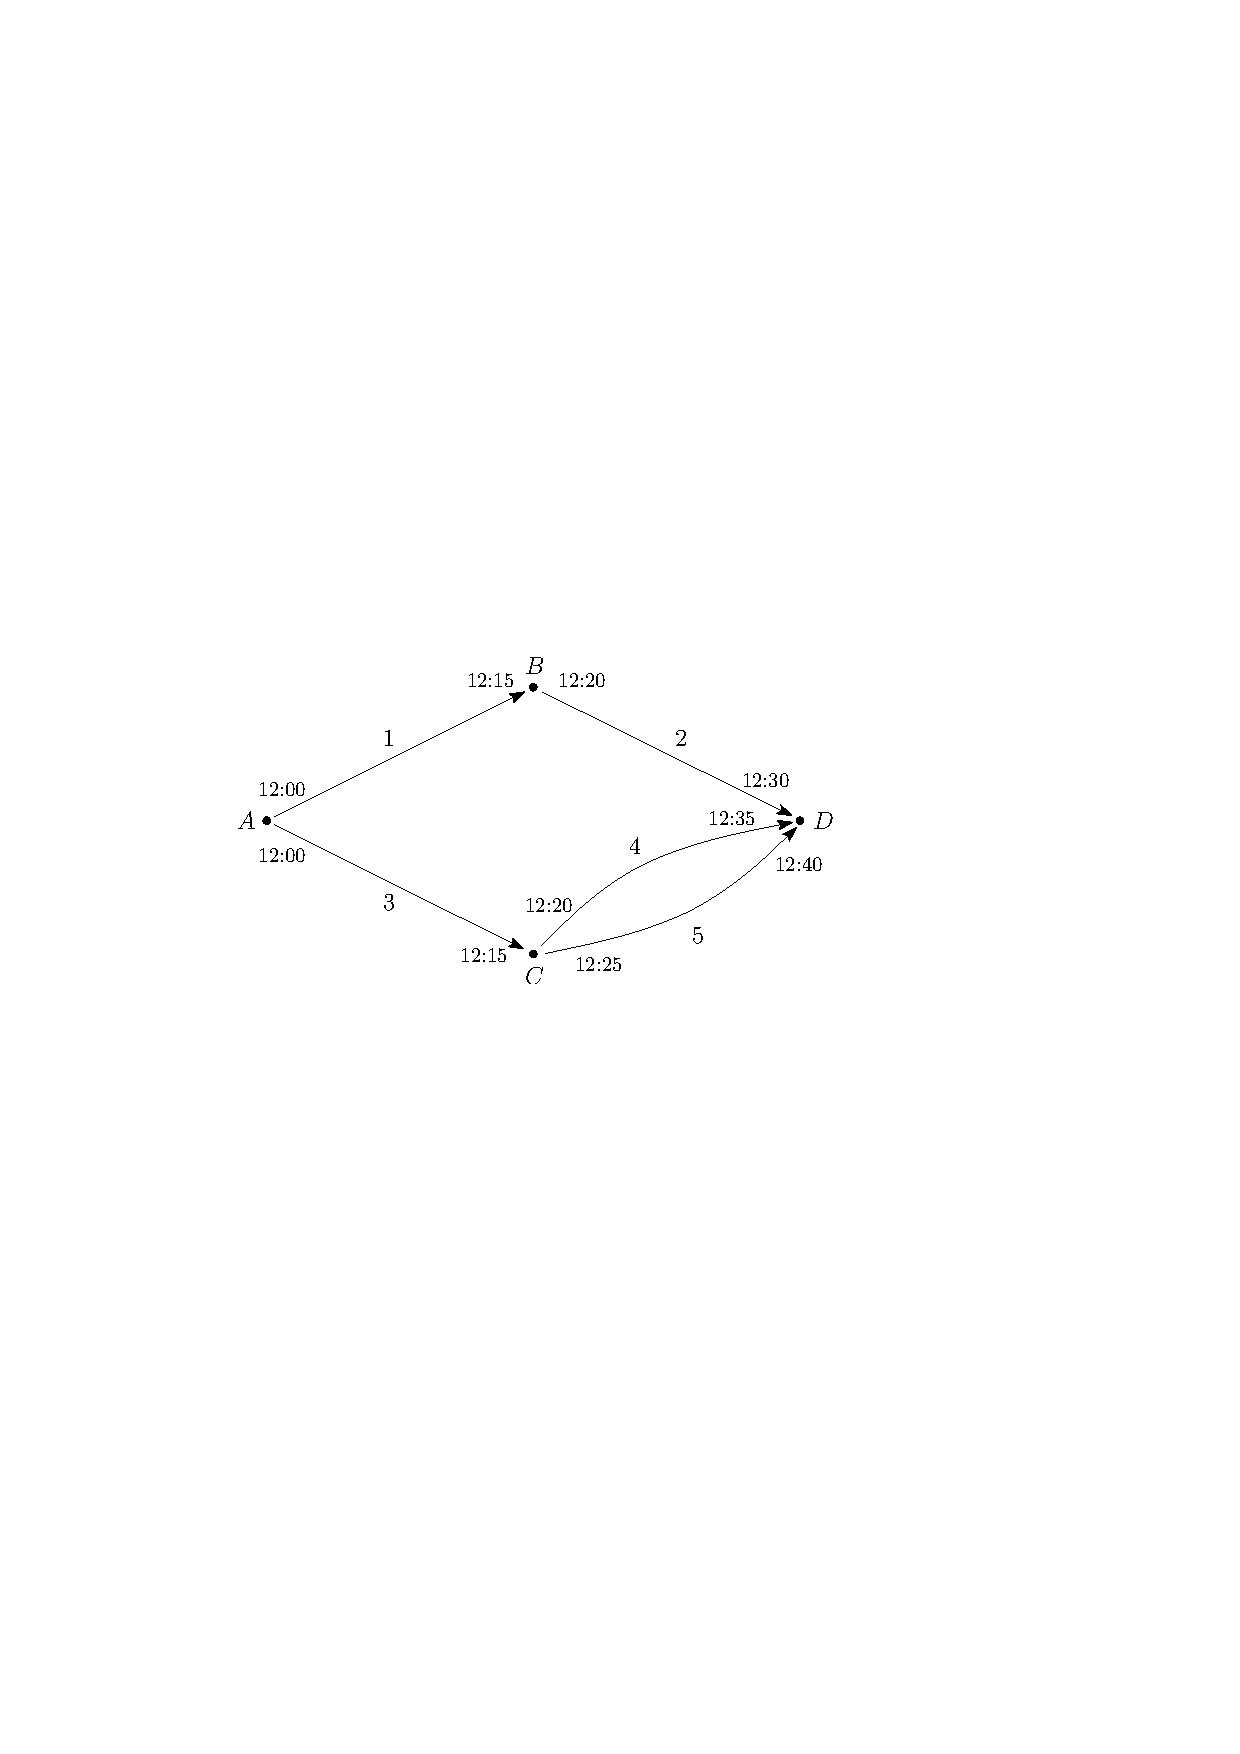
\includegraphics[width=0.7\columnwidth]{stokvsdet01}
\end{center}
\caption{The difference between stochastic and deterministic journey planning for a commuter 
traveling from $A$ to $D$. The four points represent public transport stops ($A,B,C,D$) and 
the arrows between them represent public transport services ($1,\ldots,5$).
Initially, there are three possible journeys from $A$ to $D$: $(1,2),(3,4)$ and $(3,5)$.
If the commuter initially chooses service $1$, the success of the journey is 
dependent of the success of the transfer from $1$ to $2$ at stop $B$. If the commuter chooses
service $3$ first, the destination is reached if one of the transfers $3 \to 4$ or $3 \to 5$
is successful at stop $C$.
}
\label{stokvsdet01}
\end{figure}

A simplified example clarifying the main difference between dynamic and a priori journey planning is 
shown in Figure \ref{stokvsdet01}. 

Generally, a commuter wishes to travel from an origin node $v_o$ 
to a destination node $v_d$ within a time horizon $[0,T]$ using different transport services.
Each transport service is represented as a sequence of \emph{legs}. Each leg is associated
with a \emph{start node} and \emph{end node}, as well as a random \emph{start time} and \emph{end time}.
Adjacent nodes in the network are connected with similarly defined walking legs. %, as in \cite{zografos}.

A path from the origin to the
destination is represented as a sequence of legs, in which the start node of
each leg is equal to the end node of the previous leg.
We assume that during the execution of a leg, 
the commuter receives information on which
services have already visited the end node %stop $v_i'$ 
and which are yet to arrive.
In other words, the customer ``sees'' the available successor legs of the current leg
and may choose to (i) stay in the vehicle, %if leg $i$ is not the last leg of the service, 
(ii) transfer to another vehicle or (iii) get off the vehicle and start
walking towards a nearby stop (or the destination).
The goal the above context is to determine an optimal policy specifying the actions
that are executed in different situations in order to 
optimize reliability, ride time, waiting time, walking time, the number of transfers
of a combination of these objectives.

Dynamic path finding problems (see \cite{hall,bander2002,fu1998,miller-hooks2000,davies,kim2005a,kim2005b,azaron,ferris,thomas,waller}) are often modeled
as \emph{Markov decision processes} \cite{psaraftis93,polychronopoulos}, in which the 
\emph{actions} of a decision maker at a given \emph{state} are independent of all previous actions and states.
\ref{jdjuejor} presents a conditional Markov model, in which the path history is included in each state by
defining states as sequences of legs in the transport network.
That is, the current state is determined by the path taken so far.
This model is further approximated in \ref{jtoits}, where the current state is defined as the current leg.

% The demand-responsive transport service currently being planned to operate in Helsinki
% is designed to operate on a demand-responsive basis, that is, 
% vehicle routes are modified according to the demand situation. The main difference to existing services is 
% that no pre-order times for trips are required and the trips can be booked
% ``on the fly'' by means of an interactive user interface. 
% This type of new service calls for a journey planner that is
% capable of communicating with flexible services as well as traditional
% public transport, thus combining the benefits of both transport modes.

In addition to public transport, a journey planning problem with a similar objective 
arises in freight transportation by for-hire carriers. 


\section{Stochastic model of a scheduled network [\ref{jtoits}]}
Let $\mathcal{V}$ denote a set of \emph{nodes} representing public transport stops
in a specific area and let $\mathcal{K} \subset \mathbb{N}$ denote a set of public 
transport \emph{services} operating in this area, indexed by natural numbers. 

%Let us consider the transport network during a time horizon $[0,T] \subset \mathbb{R}$.
%During this period of time, e
The route of each service $k \in \mathcal{K}$ is represented as a sequence of nodes $(v_1^k,\ldots,v_m^k)$ in $\mathcal{V}$. 
Service $k$ departs at node $v_1^k$ at a specific time and proceeds to nodes $v_2^k, \ldots,v_m^k$ in the order determined by the route.
% Due to uncertainty in departure and travel times, we define the arrival times of services at nodes
% as real-valued random variables. 
The \emph{expected passing time} of service $k$ at node $v_j^k$ is denoted by $t_j^k$.
Thus, a service $k$ can be represented as a sequence of nodes and expected passing
times $((v_1^k, t_1^k), \ldots, (v_m^k, t_m^k))$, see Figure \ref{stokvsdet02}.
% The expected arrival times $\tau_j^k$ of services at stops are assumed to be independent
% random variables. For a more detailed analysis in which the arrival times are not necessarily independent, 
% see \cite{djuejor}. In this section, we examine the arrival times as arbitrarily distributed
% real random variables. In the numerical experiments discussed in Section \ref{experiments}, 
% the arrival times are defined as gamma distributed random variables, similarly as in \cite{russell}.

\begin{figure}[ht]
\begin{center}
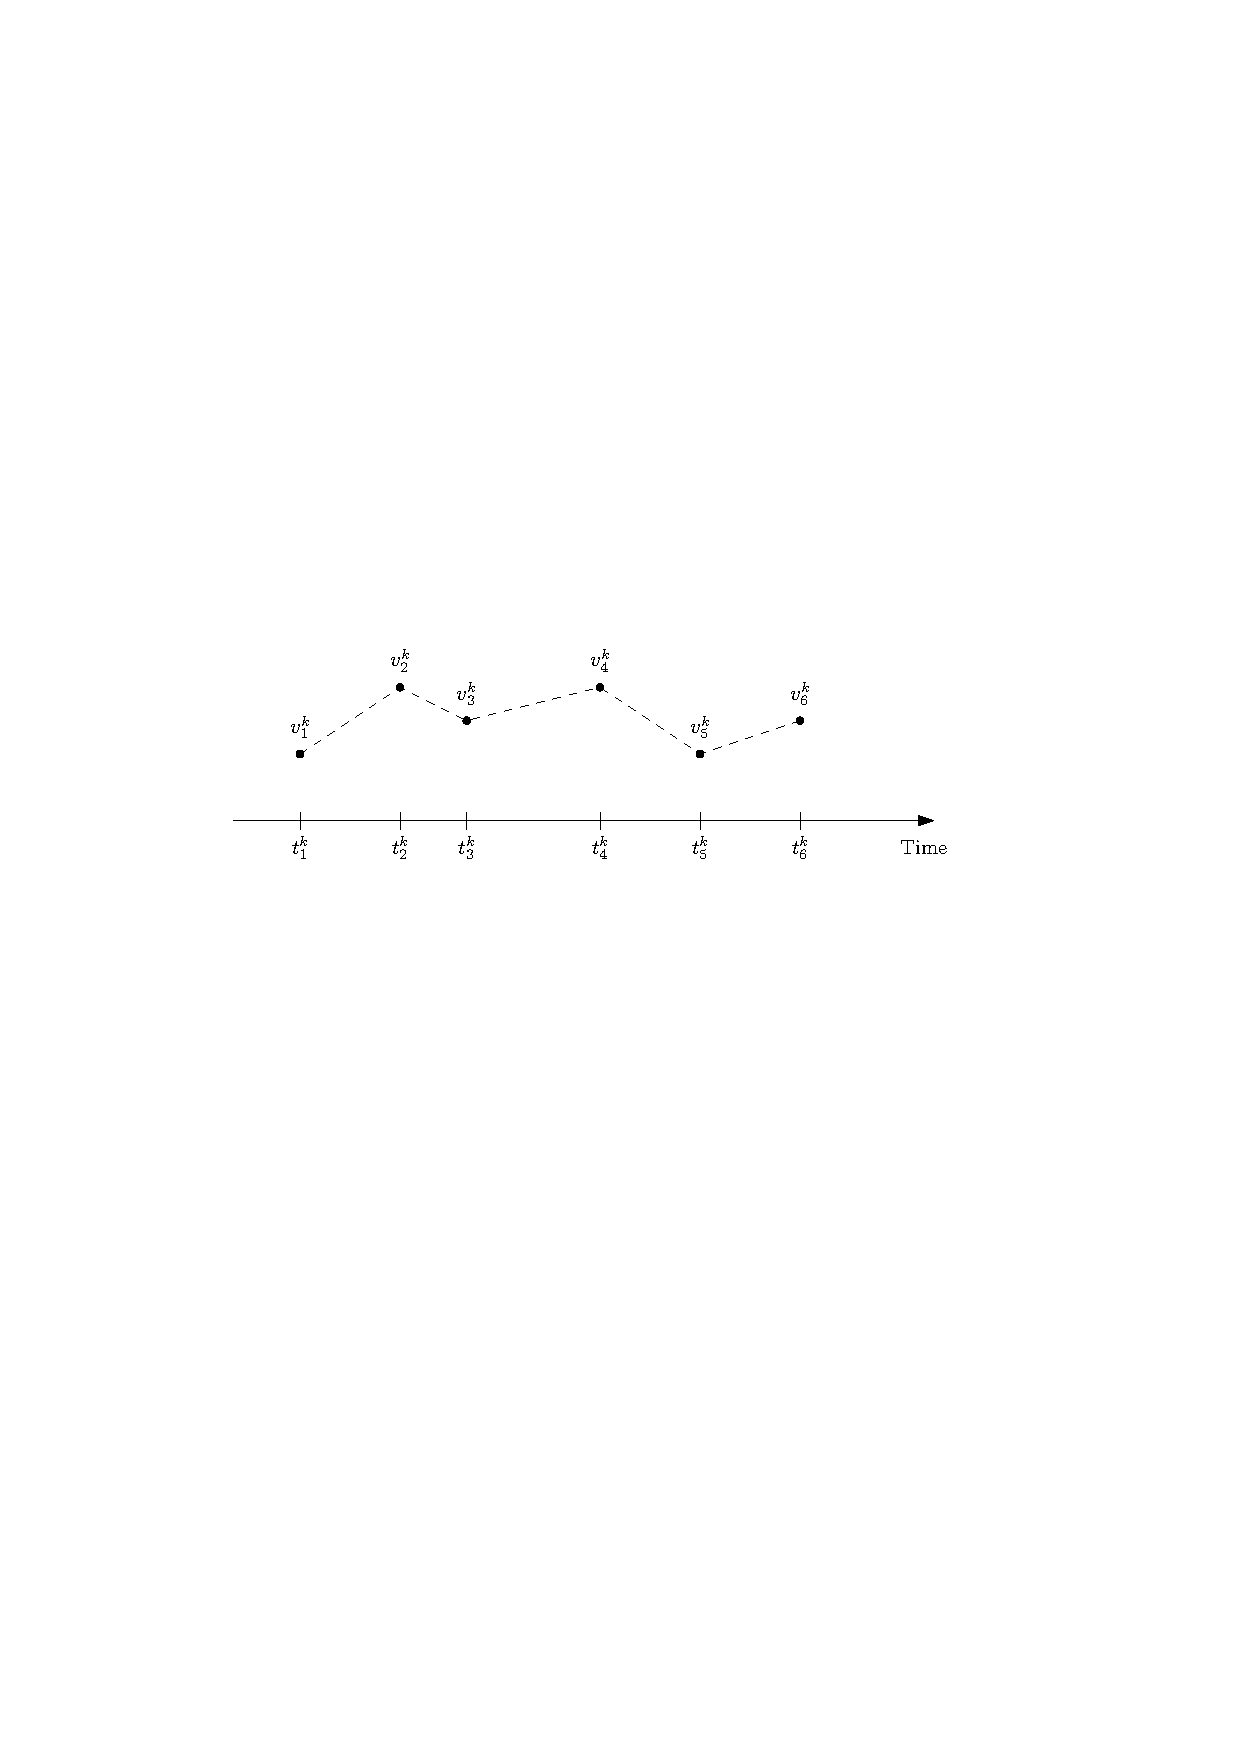
\includegraphics[width=0.8\columnwidth]{stokvsdet02b}
\end{center}
\caption{The route and schedule of a transport service. The points represent the nodes $v_j^k$ that define 
the route of service $k$ and the real numbers $t_j^k$ on the timeline represent the expected passing
times of the service at the nodes.}
\label{stokvsdet02}
\end{figure}

\subsection{Service legs and walking legs}
Each service $k \in \mathcal{K}$ is decomposed as a set of scheduled \emph{legs} between subsequent stops.
That is, each leg has a start node, end node, expected start time and expected end time.
By this decomposition, any path in the transport network can be represented as a sequence 
of legs. 
% For example, 
% the sequence $(1,2,7,10)$ defines a path involving three transfers in a transport network consisting of legs
% numbered from $1$ to $10$, see Figure \ref{etappiesim}. Each transfer between two legs has a specific probability of success.
% %Transfers between subsequent legs of the same service are assumed to be successful with 
% %probability $1$.
% 
% \begin{figure}[ht]
% \begin{center}
% 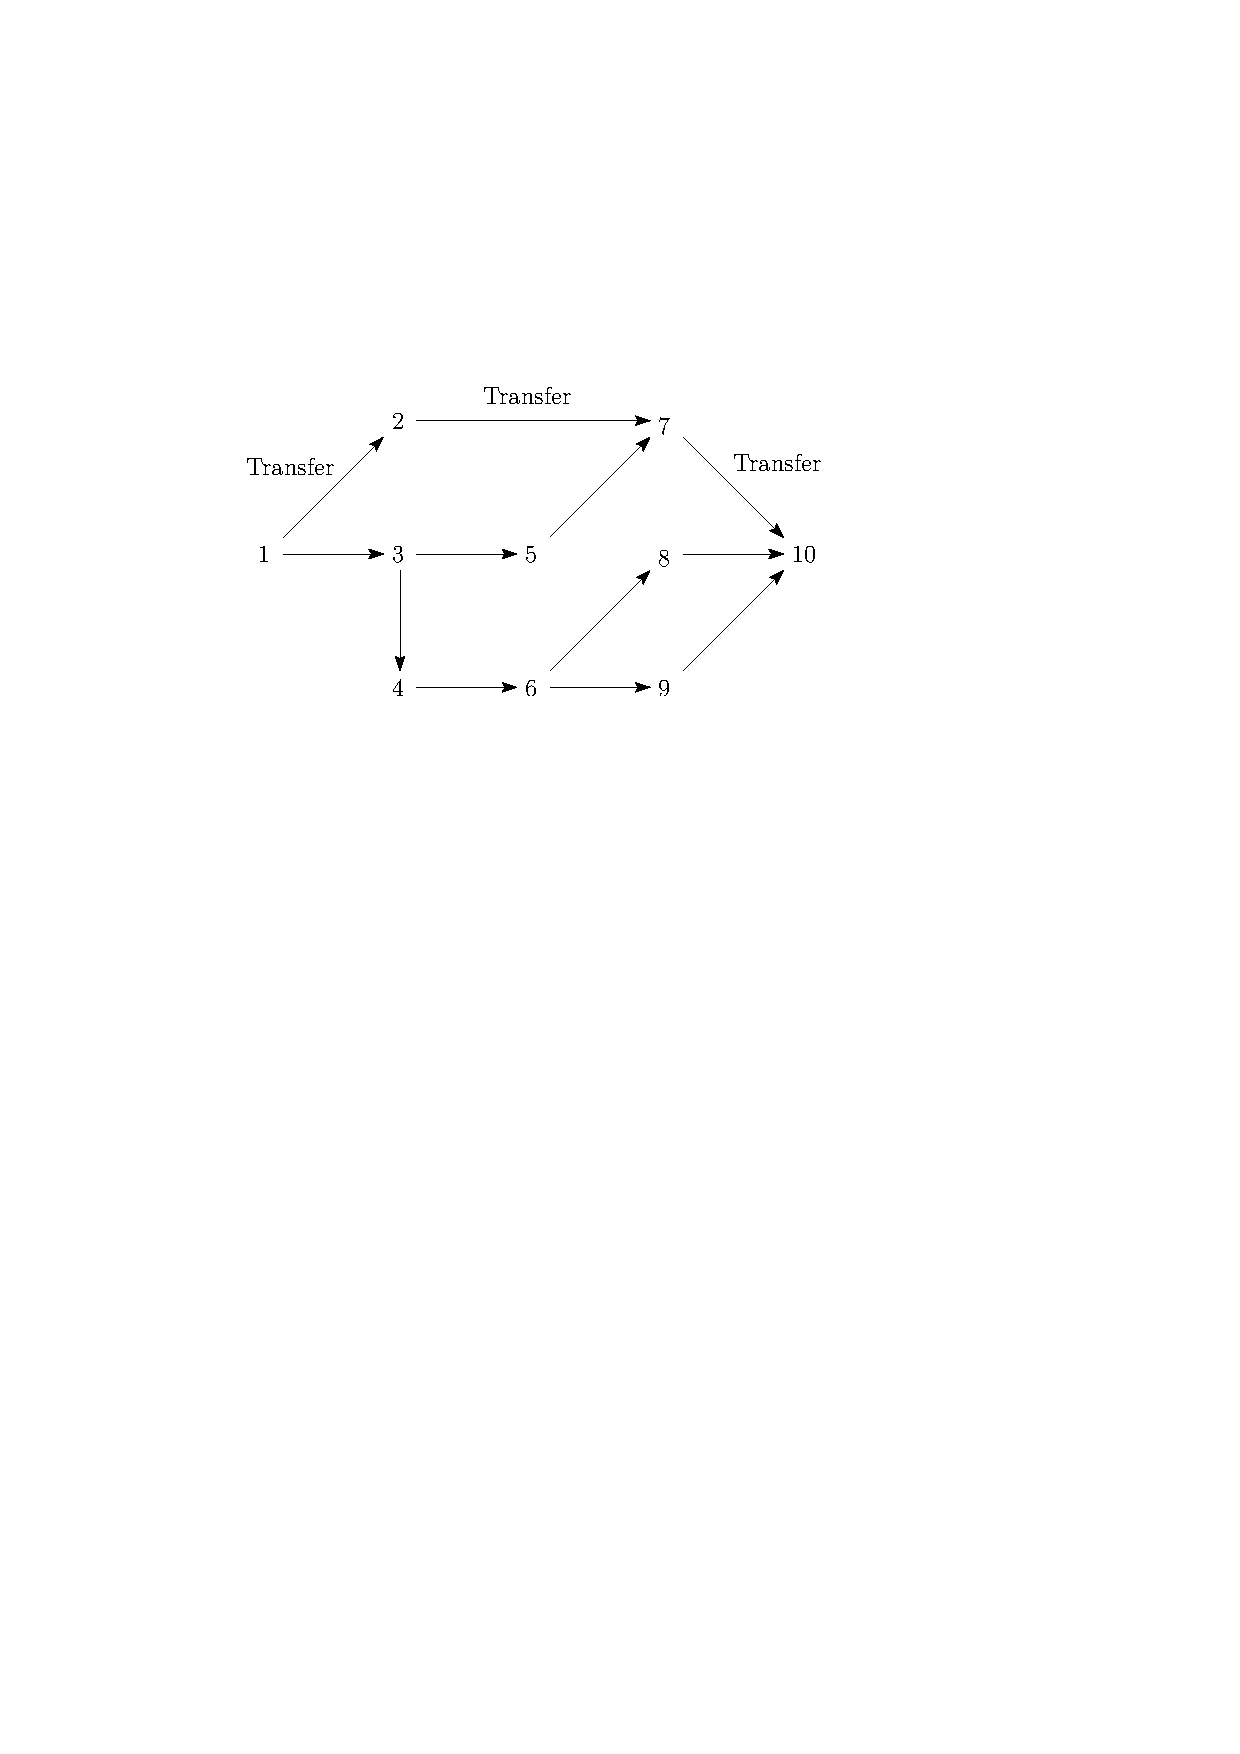
\includegraphics[width=0.5\columnwidth]{etappiesim}
% \end{center}
% \caption{A sample transport network consisting of legs numbered from $1$ to $10$. 
% The sequence $(1,2,7,10)$ defines a path involving three transfers denoted by arrows. 
% Each transfer between two legs has a specific probability of success.}
% \label{etappiesim}
% \end{figure}

After each service leg, the commuter may choose to continue the journey by foot. 
Thus, with each service leg is associated leg a set of walking legs beginning at the end of the service leg, 
see Figure \ref{walking01}a. 

\begin{figure}[ht]
\begin{center}
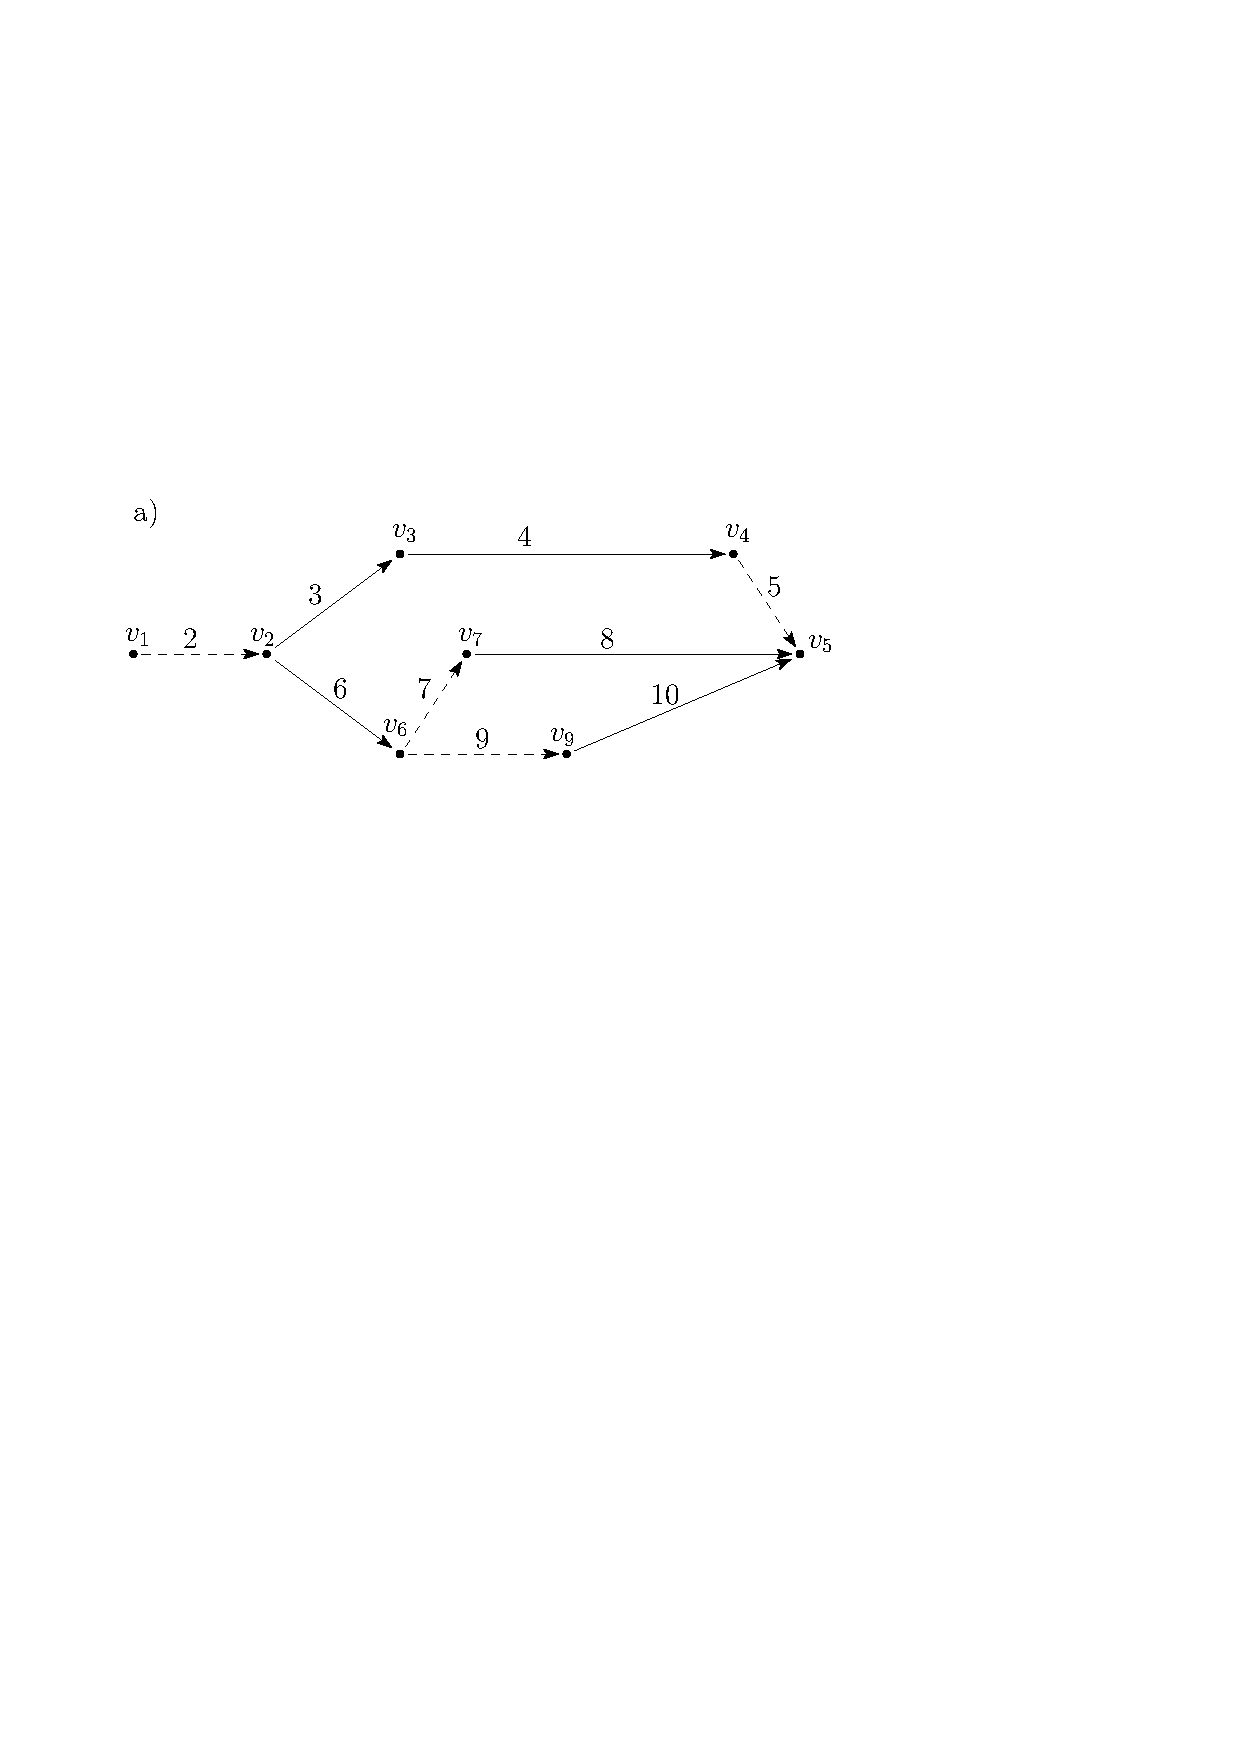
\includegraphics[width=0.45 \columnwidth]{walking02}
\hfill   
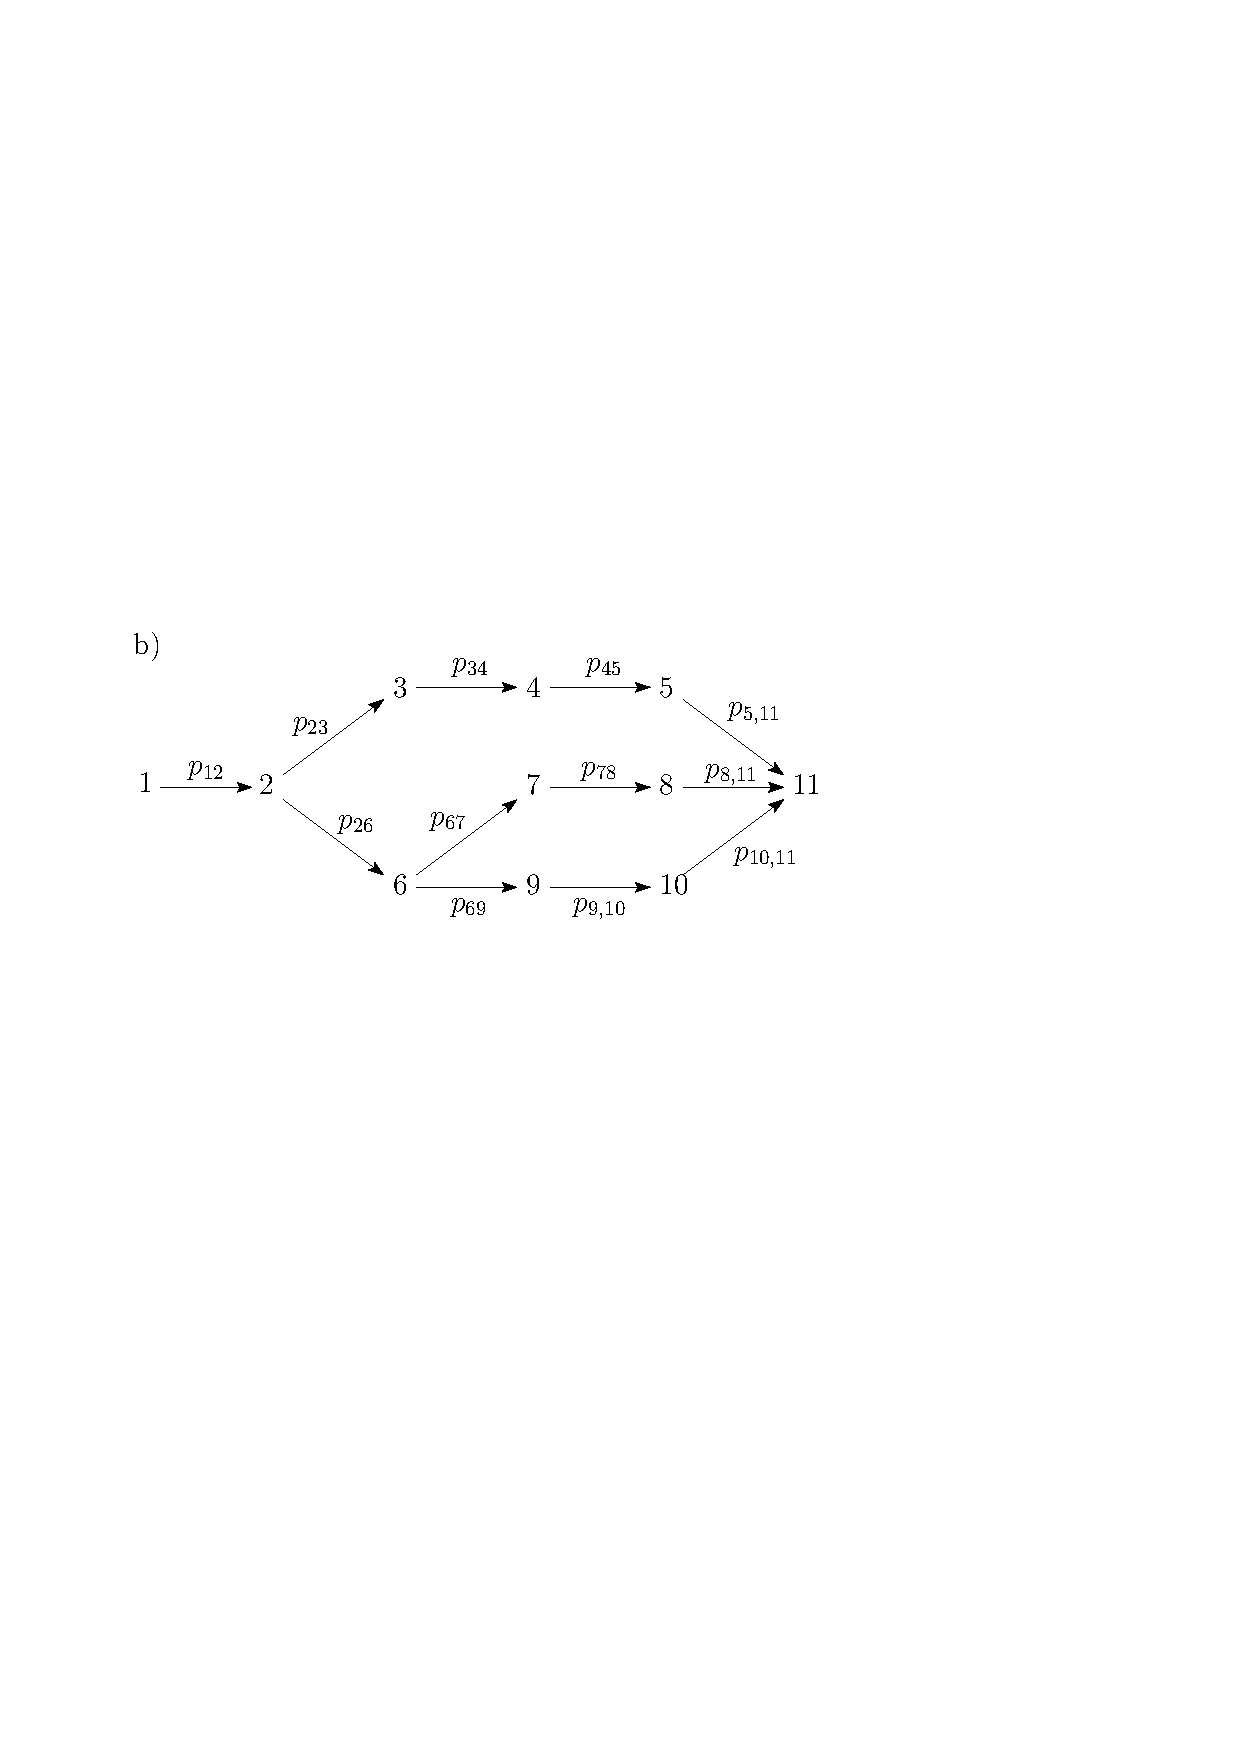
\includegraphics[width=0.45 \columnwidth]{walking02c}
\end{center}
\caption{a) A sample transport network with eight stops and five 
transport services consisting of a single leg (solid arrows $3,4,6,8,10$).
Adjacent stops are connected with walking legs (dashed arrows $2,5,7,9$).
b) A directed graph representing the relations of legs in Figure \ref{walking01}a. 
The origin and destination are represented by legs $1$ and $11$. 
The transfer probability from leg $i$ to leg $j$  is denoted by $p_{ij}$.
Note that $p_{12}=p_{45}=p_{67}=p_{69}=1$, since $2,5,7$ and $9$ are walking legs.
}
\label{walking01}
\end{figure}


\subsection{Transfers}
A transfer from leg $i$ to leg $j$ is possible only if leg $j$ begins at the node from which $i$ ends.
Letting $\mathcal{L}$ denote the set of legs and $S_i$ denote the 
\emph{successor set} of leg $i$,
the \emph{transfer probability} from leg $i$ to leg $j$ is defined as a real number $p_{ij}$ satisfying
\begin{align}
\label{transferprob}
p_{ij}
\left\{
\begin{array}{ll}
= 1, & \mbox{if $j \in S_{i}$ and $k_j < 0$ \ \ ($j$ is a walking leg)}, \\
\in [0,1], & \mbox{if $j \in S_{i}$ and $k_j > 0$}, \\ %\setminus I_i$}, \\
0, & \mbox{otherwise.}
\end{array}
\right.
\end{align}
% Note that if $j$ is a walking leg beginning at the end of leg $i$
% or if $i$ and $j$ are successive legs of the same service,
% by definition we have $p_{ij}= 1$, since $\tau_{i}'$ and $\tau_{j}$ refer to the same random variable. 
Clearly, the legs and transfer probabilities
form a directed acyclic graph, as in \cite{psaraftis93}, see Figure \ref{walking01}b. 
For analysis, we assume that the transfers between legs are independent events.

Note that transfers to walking legs are always possible. However, the success probability 
of a transfer between successive legs of the same service may be less than one due to vehicle breakdowns.
Moreover, in the determination of transfer probabilities,
one should take into the account the fact that the breakdown of a vehicle running on rail tracks blocks the way for
other vehicles using the same tracks.

% Finally, we note that the transition probabilities $p_{ij}$, where $j$ is a service leg, depend on crowding (``fail-to-sit'' probabilities)
% as in \cite{hamdouch} and \cite{schmocker}. For clarity, in the numerical experiments 
% discussed in Section \ref{experiments}, the effect of crowding is not taken into account.

\subsection{Paths}
A path can be represented as a sequence of legs $(i_1,\ldots,i_m)$ satisfying
$i_{h+1} \in S_{i_h}$ for all $h \in \{1,\ldots,m-1\}$, see Figure \ref{journey01}. 
The path is \emph{successful} with probability $\prod_{h=1}^{m-1}p_{i_hi_{h+1}}$ and the \emph{subjective price} $C \left( (i_1,i_2,\ldots,i_m) \right)$  of
the path is defined as a linear combination of expected waiting time, number of transfers, expected ride time, expected walking time and reliability. 

\begin{figure*}[ht]
\begin{center}
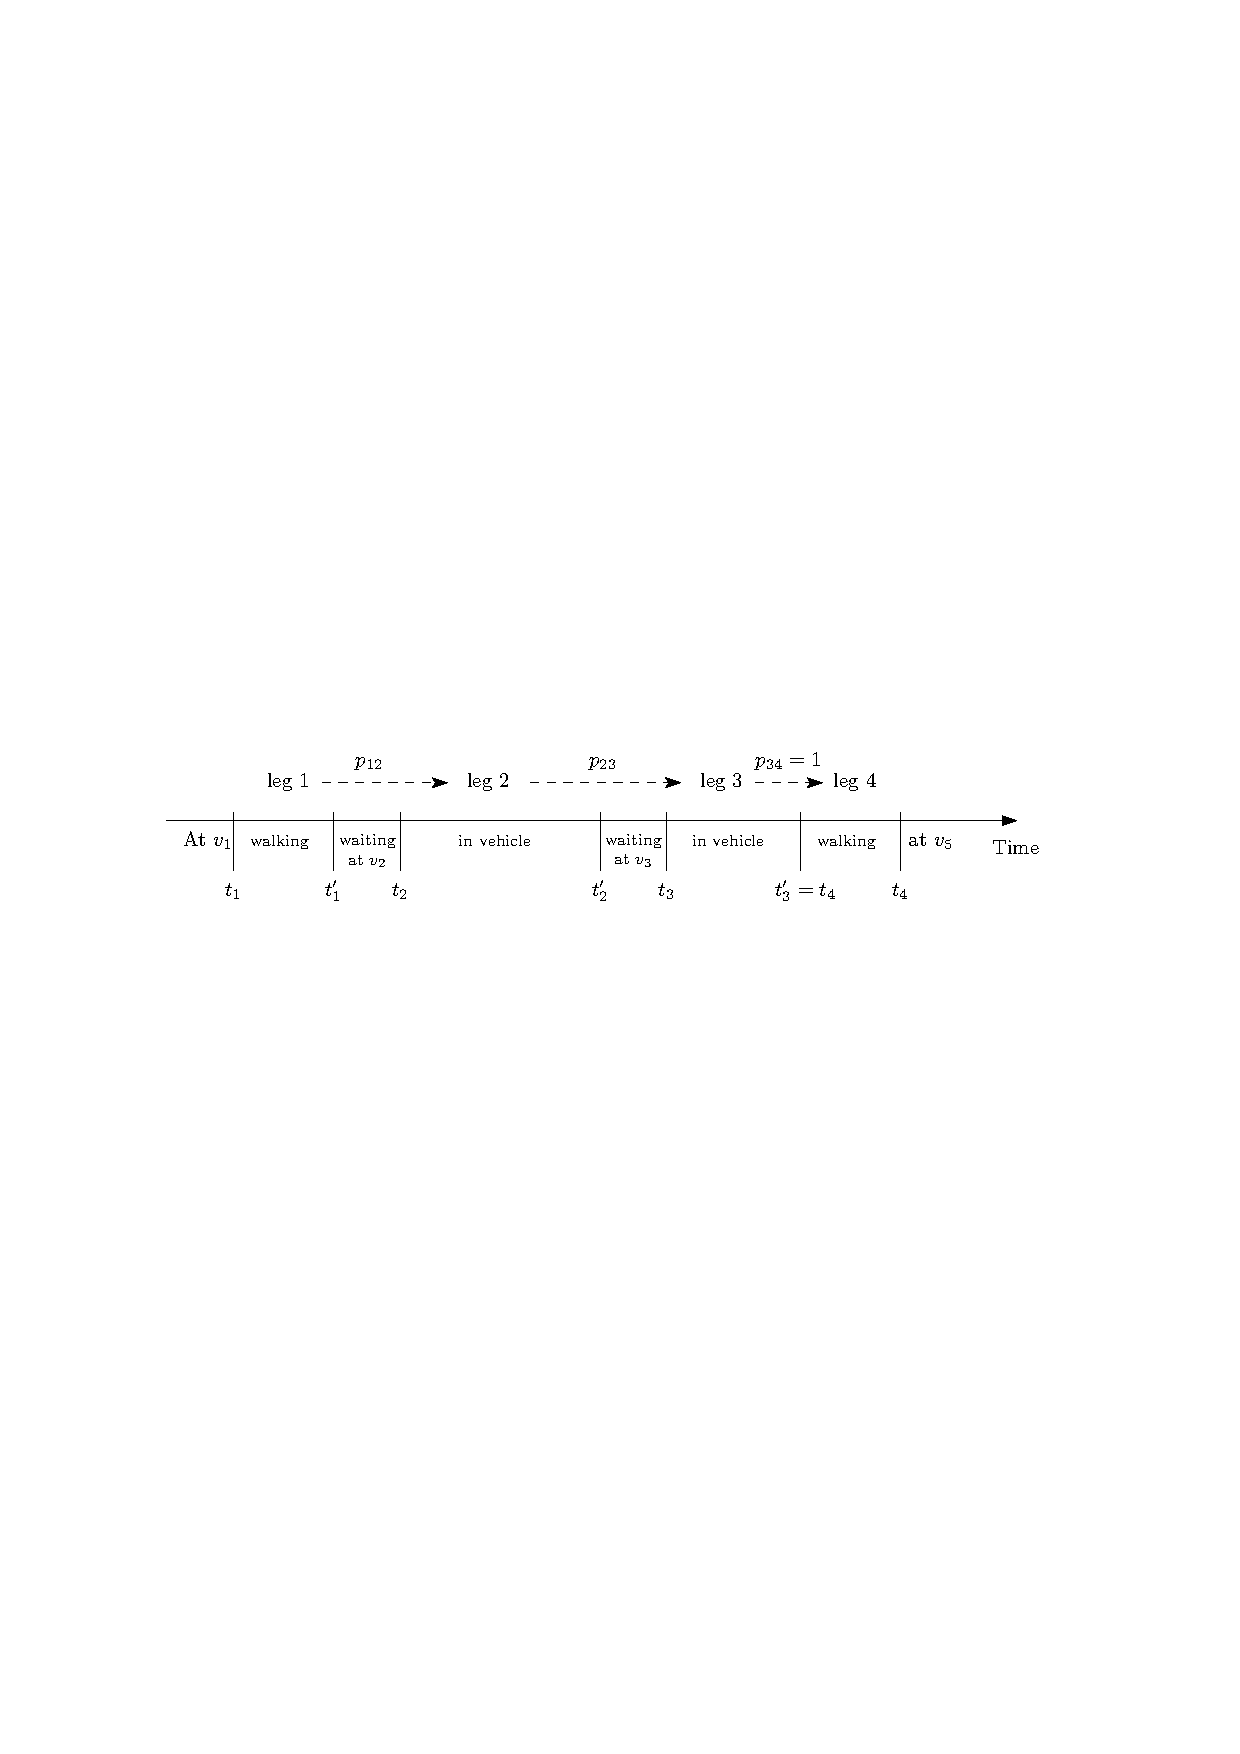
\includegraphics[width=0.8\columnwidth]{journey02b}
\end{center}
\caption{Representation of a path. The ticks on the time axis denote the 
schedule of a path from $v_1$ to $v_5$. The path is represented by four legs: 
1) A commuter starts walking from the origin $v_1$, and arrives at stop $v_2$. 
2) A transport service departs at $v_2$ and travels to stop $v_3$. 
3) A transport service departs at $v_3$ and arrives at stop $v_4$. 
4) The commuter continues by foot to the destination $v_5$. Note that the path is successful
with probability $p_{12}p_{23}$.
}
\label{journey01}
\end{figure*}

%In addition,
%for walking legs $l_j$ for which $j > 1$ it is required that $\tau_{l_j} = \tau_{l_{j-1}'}$.
%In other words, each walking leg begins as soon as the preceding leg is completed.

% \subsection{Time horizon}
% \label{problem}
% %The dynamic journeying problem is defined as follows.
% Let $[0,T] \subset \mathbb{R}$ be the time horizon of the problem.
% % let $v_1$ denote the origin node and $v_d$ denote the destination node. 
% % The \emph{origin leg} is defined by $((v_1,0),(v_1,0),0)$, 
% % and the \emph{destination leg} 
% % is defined by $((v_{d},T),(v_{d},T),0)$.
% % By the above definitions, we can represent the entire journey 
% % as legs, including the origin and the destination. 
% % 
% % With no loss of generality, 
% All legs for
% which the expected start or end time is outside the time horizon $[0,T]$ and 
% all legs for which the start node is the destination node (except the destination leg)
% are excluded from the problem.
% The cropped set of legs is denoted by $\mathcal{L}_{[0,T]}$.
% For clarity, we define $n:=|\mathcal{L}_{[0,T]}|$ and the legs in $\mathcal{L}_{[0,T]}$ 
% are numbered from $1$ to $n$, where the origin leg is indexed by $1$ and the destination leg is indexed by $n$.

\section{Problem solution}
In Section \ref{mdp}, we model the journeying problem as a Markov Decision Process and propose an algorithm 
for maximizing the general objective function.
In Section \ref{hits}, we present a simplified algorithm for maximizing the reliability of a journey.
%by maximizing the expected number of successful paths to the destination. 
%In the second approach (Section \ref{mdp}), we consider a 
%more general objective function by modeling the problem as a Markov decision process.

\subsection{Markov Decision Process}
\label{mdp}
In order to be able to handle a general objective function,
we propose a finite-state Markov decision process, %$(S,A,P_{\cdot}(\cdot,\cdot),R_{\cdot}(\cdot,\cdot))$, 
%where the parameters are defined as follows.
%The general approach to the problem 
where the goal is to determine an optimal \emph{policy} with respect to the objective function. 

A policy defines for each leg $i \in \{1,\ldots,n-1\}$ a \emph{ranking} of successor 
legs $i' \in S_i$. 
The policy is used to choose the best transfer options during the journey as follows:
At the end of each leg $i \in \{1,\ldots,n-1\}$, the transfer options to successor legs $i' \in S_i$ are revealed. 
After the transfer options are revealed, letting $X \subset S_i$ denote the 
set of successor legs to which a transfer is possible, the commuter transfers to the 
leg $x \in X$ with the highest ranking, see Figure \ref{rankingexample}.

The above approach produces relatively easy to follow travel information, since 
the commuter knows the ranking of successor legs before each transfer. Note that the policy can be re-optimized during the journey 
if the transition probabilities between legs are updated by using real-time traffic information. That is, a new optimal policy for the 
remaining part of the journey can be calculated at $t \in [0,T]$ by using the updated transition probabilities available at $t$. 
This type of dynamically adaptive policy could be useful in situations in which there is substantial uncertainty in travel times.

 \begin{figure}[ht] 
\scriptsize
\begin{tabular}{p{3cm}c|p{2cm}|p{2cm}|}
\cline{3-4}
\multirow{5}{*}{} 
\multirow{5}{*}{
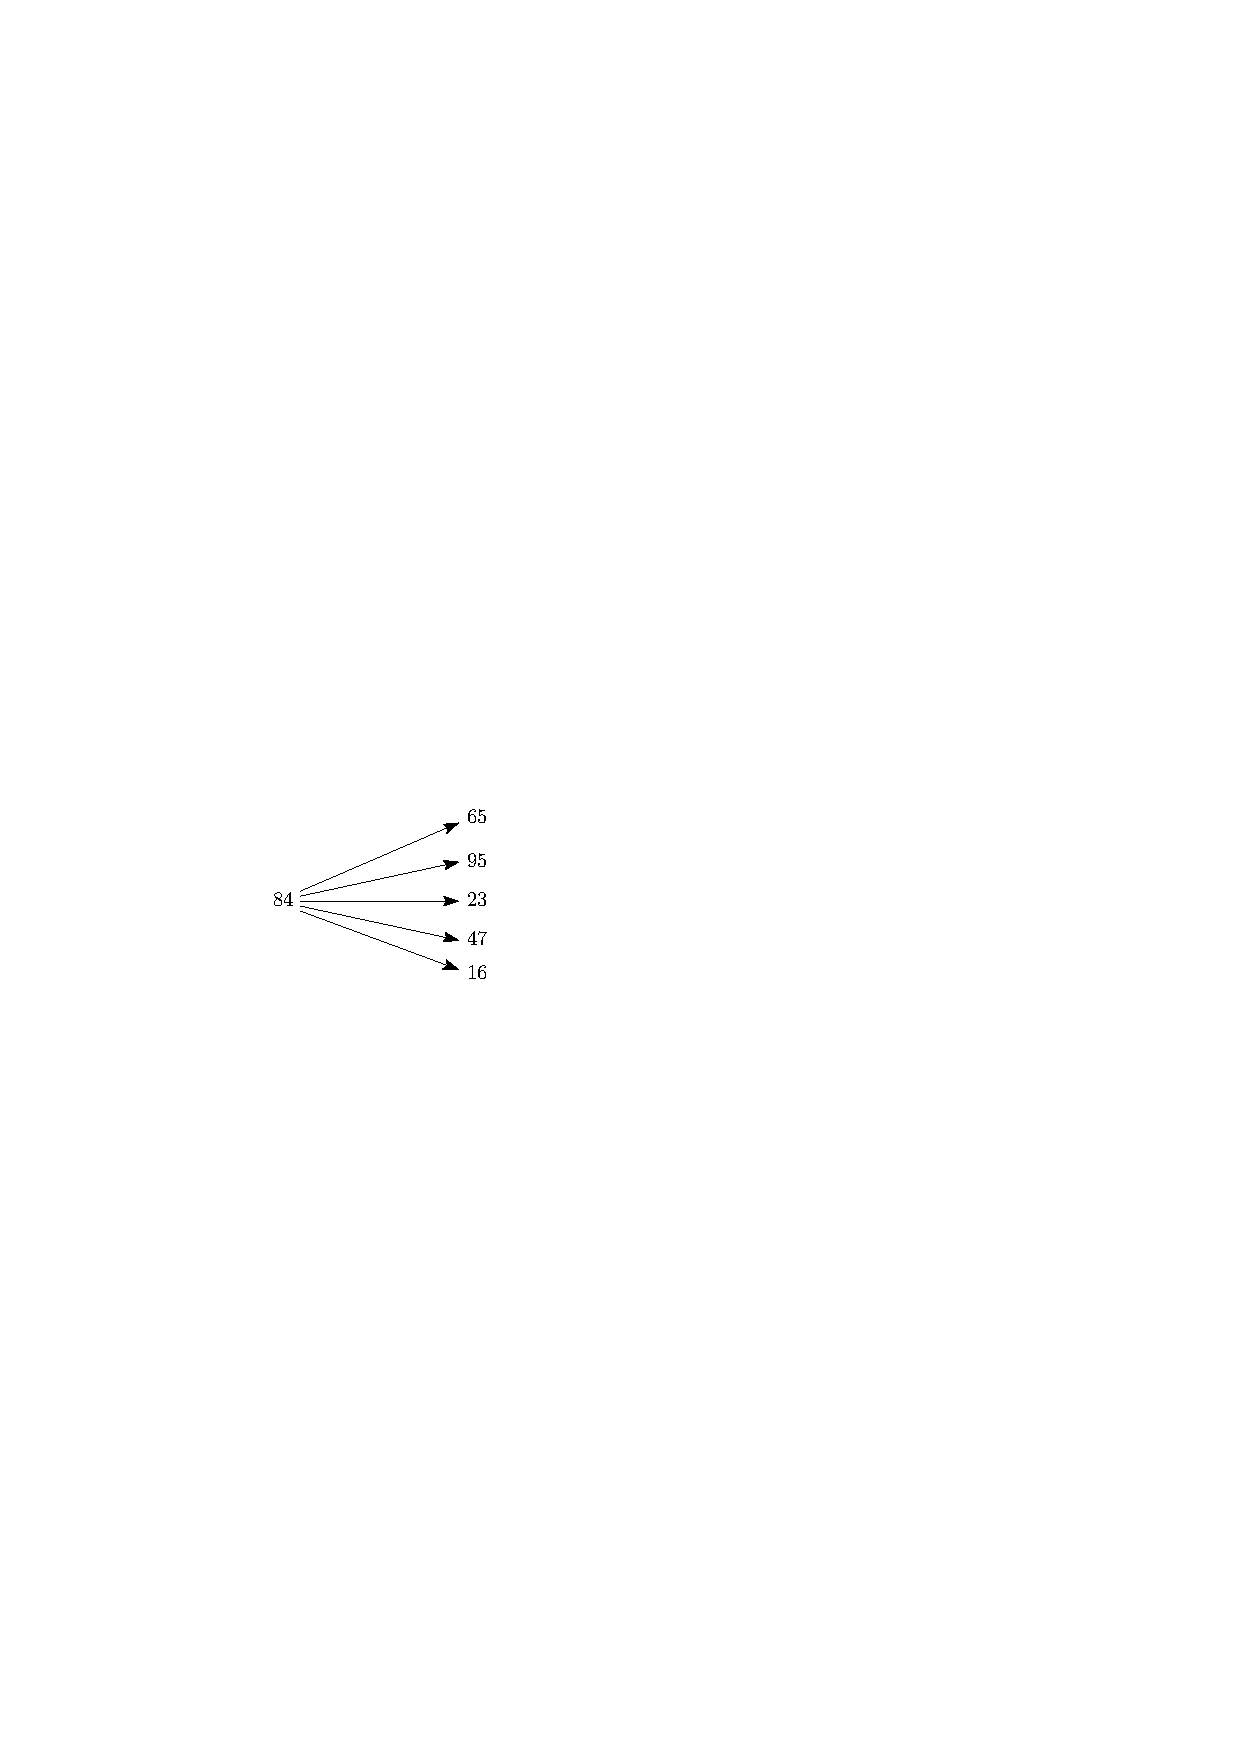
\includegraphics[width=0.305\columnwidth]{rankingexample2.pdf} 
} 
& & Ranking of successors of leg $84$ & End of leg $84$: transfer options are revealed \\
\cline{3-4}
&  \ \ \ \ \ \ \ \   \ \ \ \ \ \ \ \ & \ \ \ \ \ \ \ \ $1: 23$ & \ \ \ \ \ \ \ \ $\cancel{1:  23 }$  \\
&  \ \ \ \ \ \ \ \   \ \ \ \ \ \ \ \ & \ \ \ \ \ \ \ \ $2: 16$ & \ \ \ \ \ \ \ \ $2: 16$ $\leftarrow$  \\
&  \ \ \ \ \ \ \ \   \ \ \ \ \ \ \ \ & \ \ \ \ \ \ \ \  $3: 65$ & \ \ \ \ \ \ \ \ $\cancel{3: 65}$ \\
&  \ \ \ \ \ \ \ \   \ \ \ \ \ \ \ \ & \ \ \ \ \ \ \ \  $4: 47$ & \ \ \ \ \ \ \ \ $\cancel{4:  47 }$  \\
&  \ \ \ \ \ \ \ \   \ \ \ \ \ \ \ \  & \ \ \ \ \ \ \ \ $5: 95$ & \ \ \ \ \ \ \ \ $5: 95$  \\
\cline{3-4}
\end{tabular}
 \caption{A ranking example. %The commuter is executing leg $42$, whose successor legs are $54,24,65,32$ and $12$.
The left column of the table shows the a priori ranking of successors of leg $84$. When the commuter is at the end of leg $84$, the available transfer options
($16$ and $95$) are revealed. The commuter then transfers to leg $16$, which has the highest ranking among the possible transfer options.}
\label{rankingexample}
\end{figure}

Formally, the parameters of the Markov decision process $(S,A,P_{\cdot}(\cdot,\cdot),R_{\cdot}(\cdot,\cdot))$ are defined as follows.

\subsubsection{States $=$ Legs}
\label{statesdef}
The set of \emph{states} $S$ is equal to the set of 
legs\footnote{A more detailed model described in \ref{jdjuejor} defines states as sequences of legs.} numbered from $1$ to $n$, that is, $S= \{1,\ldots,n\}$.
State $1$ is referred to as the \emph{origin state} and state $n$ is referred to as the \emph{destination state}.
%Since legs beginning from the destination node are not included in the problem, we have $S_n = I_n = \emptyset$.



\subsubsection{Actions}
\label{actionsdef}
The set of \emph{actions} $A$ consists of sets $A_s$ of actions available at states $s \in S$.
An action $a \in A_s$ is defined as a \emph{preference order} of the successor states $s' \in S_s$, 
that is, a bijection $a:S_s \to \{1,\ldots,|S_s|\}$, where $a(s')$ denotes the ranking of the successor state $s' \in S_s$
in the preference order. The successor states of $s$ ranked by the preference order $a$ are denoted by $s^{a,a(s')}$.
Given the the sorted successor states $s^{a,1}, \ldots, s^{a,|S_s|} \in S_{s}$ of $s$, 
the commuter transfers to state $s^{a,k}$ if 
(i)
the transfer to $s^{a,g}$ is unsuccessful for $1 \leq g < k$ and 
(ii)
the transfer to $s^{a,k}$ is successful.

\subsubsection{Transition probabilities}
\label{transitiondef}
$P_a(s,s')$ is the probability that action $a$ in state $s$ 
at step $t$ will lead to state $s' \in S_s$ at step $t + 1$. 
Given the preference order $s^{a,1}, \ldots, s^{a,|S_s|} \in S_{s}$ defined by action $a \in A_s$, 
since successful transfers are assumed to be independent\footnote{See \ref{jdjuejor} for a model in which the transfers between services
are not independent.} events, we have 
\begin{align}
\label{ekakaava}
P_a(s,s^{a,k}) 
= \sum_{k=1}^h p_{ss^{a,k}} \prod_{g = 1}^{k-1}(1-p_{ss^{a,g}}),
\end{align}
where $p_{ss^{a,k}}$ denotes the transfer probability from $s$ to $s^{a,k}$, as defined in Equation \eqref{transferprob}.
% Note that since the transfer probability from $s$ to an immediate successor state $s' \in I_s$ satisfies
% $p_{ss'} = 1$, the transfer probability \eqref{ekakaava}
% satisfies $P_a(s,s^{a,k}) = 0$ if $\{s^{a,1},\ldots,s^{a,k-1}\} \cap I_s \neq \emptyset$, and
% $P_a(s,s^{a,k}) = {\prod_{g = 1}^{k-1}(1-p_{ss^{a,g}})}$ if $\{s^{a,1},\ldots,s^{a,k-1}\} \cap I_s = \emptyset$ and $s^{a,k} \in I_{s}$. 
%For example, let $s^{a,1},s^{a,2},s^{a,3}$ denote three successor states of state $s$, sorted in the preference
%order defined by action $a$. If $s^{a,2}$ is an immediate successor of $s$, that is, $s^{a,2} \in I_s$, and $s^{a,1} \notin I_s$, 
%we have $P_a(s,s^{a,1}) = p_{ss^{a,1}}$, $P_a(s,s^{a,2}) = 1-p_{ss^{a,1}}$
%and $P_a(s,s^{a,3}) = 0$.

\subsubsection{Rewards}
\label{rewardsdef}
$R(s,s')$ is the expected immediate reward received after transition from state $s \in S$ to state $s' \in S$ 
with transition probability $P_a(s,s')$. Since the objective is to minimize the subjective price of the trip, $R(s,s')$ is defined 
as the difference in subjective price due to the transition from $s$ to $s'$.

 
% The expected profit of a path $(1,s_1,\ldots,s_{m},n)$ from the origin state $1$ to the destination state $n$
% is given by 
% \begin{align}
% \label{expectedprofit}
%  &\pi \left((s_0,\ldots, s_m) \right) 
% = p_{s_{m}n} u - C \left((s_0,\ldots, s_m) \right),  
% \end{align}
% where $u$ is the utility of arriving at the destination before the deadline $T$ (or at $T$) 
% and $C \left((s_0,s_1,\ldots,s_{m-1}, s_m) \right)$
% is the subjective price of the path.
% 
% Since the objective is to maximize \eqref{expectedprofit}, we define $R_a(s,s')$ by
% \begin{align}
% \label{rewards}
%  R_a(s,s')= 
% \left\{
% \begin{array}{ll}
% u, &  \mbox{if $s' = n$ },\\ 
% - \Delta C(s,s'), & \mbox{otherwise,}
% \end{array}
% \right.
% \end{align}
% where $\Delta C(s,s')$ denotes the increase in the subjective price.
% Note that $R_a(s,s')$ is independent of the action $a$. Thus, for the remainder of this chapter, we will use
% the notation $R(s,s') = R_a(s,s')$.
% 
% Clearly, the above model can be used to maximize the probability of arriving at the destination in
% time by defining $u=1$ and $\Delta C(s,s') = 0$. That is, the commuter receives reward $1$ upon arrival at the 
% destination state and the rewards of transitions to other states are equal to zero.

\subsection{Optimal policy}
\label{solution}
The solutions to Markov decision processes are characterized as policies, 
that is, functions $\pi$ that specify the action 
$a(s) $ that the commuter chooses when in state $s$. 
%Note that a policy $\pi$ fixes the action for 
%each state and the behaves like a Markov chain.
The goal is to find an optimal policy, that is, a policy that maximizes the expected reward. 
%in this case, the probability of reaching a destination state $s \in \mathcal{D}$.
Generally, the calculation of an optimal policy requires two arrays indexed by state: 
value $V$, which contains real values, and policy $\pi$ which contains actions. 
%At the end of the algorithm, $\pi$ contains the solution and $V(s)$ contains the expected 
%rewards to be earned on average by following that solution from state $s$.
The value $V(s)$ of $s$ corresponds to the expected rewards to be earned by following a 
policy that maximizes the expected rewards from $s$ onwards.

Reference \cite{bellman} defines the value $V(s)$ by 
\begin{align}
\label{value}
V(s) := \max_{a \in A_s} \left\{ \sum_{s' \in S_s} P_a(s,s') \left(R(s,s') +V(s')\right)\right\}
\end{align}
for all $s \in S$. Note that $V(n)=0$ since $S_n = \emptyset$.

An optimal policy is characterized as follows:
When at state $s$, the available transfer options $R \subset S_s$ to successor states are revealed.
The commuter transfers to a state $s' \in R$ for which $R(s,s') +V(s')$ is maximized.
Thus, an optimal action $a$ at state $s$ is defined by %the as follows.
%determined by the following theorem.
%\begin{theorem}
%\label{optimalpolicy}
%Let $s \in S$ be a state. An action $a \in A_s$ is optimal satisfying Equation \eqref{value}, if 
%the preference order $s^{a,a(s')}$ of the successor nodes $s' \in S_s$ 
%satisfies 
\begin{align}
\label{jarjestys}
R(s,s^{a,1})+V(s^{a,1}) \geq \ldots \geq R(s,s^{a,|S_s|})+V(s^{a,|S_s|}),
\end{align}
where the successor states ranked by action $a$ are denoted by $s^{a,a(s')}$ for all $s' \in S_s$.
%\end{theorem}
%The proof of Theorem \ref{optimalpolicy} is given in \cite{djuejor}.
% \begin{proof}
% Let $S_s = \{s^1,\ldots,s^{|S_s|}\}$ denote the successor set of state $s$.
% Given an arbitrary realization $\{ \tau_s'=t_s',\tau_{s^1} = t_{s^{1}},\ldots,\tau_{s^{|S_s|}} = t_{s^{|S_s|}} \}$ of
% the end time of state $s$ and the start times of states $s^k \in S_s$,
% the conditional value of $s$ satisfies
% \begin{align*}
% V(s \mid t_s', t_{s^{1}}, \ldots , t_{s^{|S_s|}}) = 
% \max_{ \{k \in \{1,\ldots,|S_s|\} \ | \ t_{s}' \leq t_{s^{k}} \}}
%  \left\{ R(s,s^{k}) +V(s^{k}) \right\}.
% \end{align*}
% Note that $t_{s^k} = t_s'$ for all $s^k \in I_s$.
% Let $a$ be an action satisfying Equation \eqref{jarjestys}.
% Since the conditional transition probability is given by
% \begin{align*}
% P_{a}(s,s^{a,k} \mid t_s', t_{s^{a,1}}, \ldots , t_{s^{a,|S_s|}}) = 
% \left\{
% \begin{array}{ll}
% 1, & \mbox{if $t_s' \leq t_{s^{a,k}}$ and $t_s' > t_{s^{a,g}}$ for $1 \leq g < k$},\\
% 0, & \mbox{otherwise},
% \end{array}
% \right.
% \end{align*}
% we have
% \begin{align*}
% V(s \mid t_s', t_{s^{a,1}}, \ldots , t_{s^{a,|S_s|}}) 
% & =  \sum_{k=1}^{|S_s|} P_{a}(s,s^{a,k} \mid t_s', t_{s^{a,1}}, \ldots , t_{s^{a,|S_s|}}) \left( R(s,s^{a,k}) +V(s^{a,k}) \right).
% \end{align*}
% Integrating over $\mathbb{R}^{|S_s|+1}$ yields
% \begin{align}
% \label{ekakaava}
% V(s) = \sum_{k=1}^{|S_s|} P_{a}(s,s^{a,k}) \left( R(s,s^{a,k}) +V(s^{a,k}) \right).
% \end{align}
% \end{proof}
Equation \eqref{jarjestys} 
gives an optimal action for a state $s$, given that the values $V(s')$ of its successor states are known.
In the following, we present an algorithm for calculating the values for all states that are reachable from the origin state.

\subsection{Backward induction algorithm}
\label{alg01}
The values $V(s)$ of states can be determined
by means of backward induction. The recursive function Rec($s$) executes the following procedures at each recursion step:
\\

\noindent
1. Check if the value of the current state $s$ has been determined. If yes, return the value.

\noindent
2. For all successors $s'$ of the current state: Calculate the value of $s'$ by calling Rec($s'$).

\noindent
3. Determine the optimal action for the current state $s$ by ranking the successors.

\noindent
4. Calculate and return the value of the current state.
\\

By executing Rec($1$), the program recursively calculates the values and optimal actions for 
all states $s$ that are reachable from the origin state $1$.
Initially, we only know the value of the destination state, that is, $V(n)=0$.
Thus, the first states for which the value can be calculated
are the ones that precede the destination state. 
The algorithm then proceeds backwards until the value $V(1)$ of the origin state is calculated.
%An example of determining the optimal policy is depicted in Figure \ref{toyexample}.

Since the algorithm involves sorting, the complexity is bounded above by $\mathcal{O}(n m \log m + nm) = \mathcal{O}(n m (1+\log m))$,
where $m = \max_{s \in \{1,\ldots,n-1\}}|S_s|$ is the size of the largest successor set. Note that although the total number of 
possible actions for a successor set $S_s$ equals $|S_s|!$, the complexity of the algorithm is smaller due to the fact that 
the successors of each state are ordered only once. That is, the algorithm goes through all states reachable from the origin state 
but not through all possible actions. 

% \begin{figure}
% \centering{
% 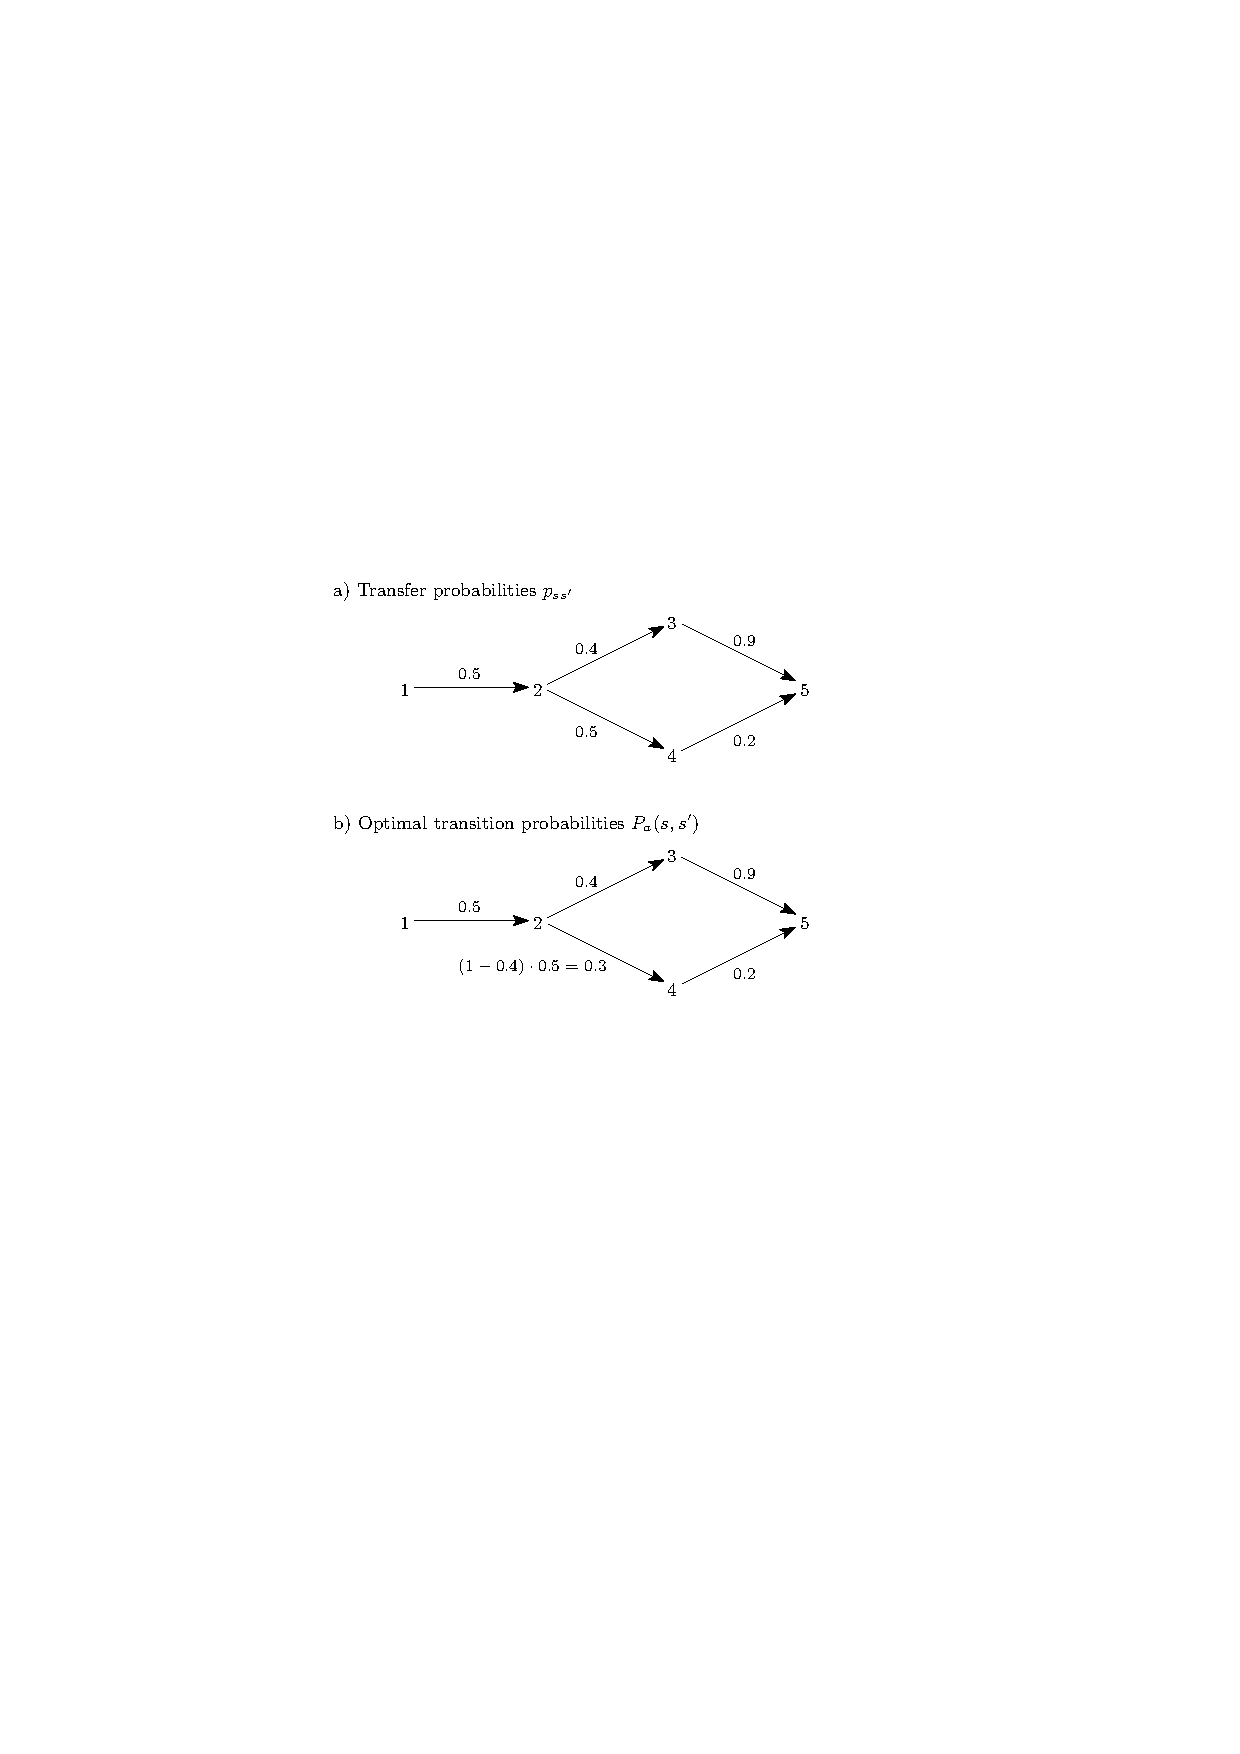
\includegraphics[width=0.7\columnwidth]{toyexample2.pdf}
% }
% \\
% \ \ \ \ \ \ \ \ \ \ \ \
% \\
% {\footnotesize
% \begin{tabular}{|p{1cm}|p{1.0cm}|p{5.5cm}|}
% \hline
% State & Optimal action & Value \\
% \hline
% 5 & - & 0 \\
% 3 & 5 & $p_{35} \cdot 1 = 0.9$ \\
% 4 & 5 & $p_{45} \cdot 1 = 0.2$ \\
% 2 & 3,4 & $p_{23} \cdot 0.9 + (1-p_{23}) p_{24} \cdot 0.2 = 0.42$\\
% 1 & 2 & $p_{12} \cdot 0.42 =0.21$ \\
% \hline
% \end{tabular}
% }
% \caption{Calculating the optimal policy with respect to the probability of reaching the destination state. 
% The top figure a) shows the states $1,\ldots,5$, where $1$ is the origin and $5$ is the destination state, and the 
% transfer probabilities $p_{ss'}$ between the states. 
% The table shows the states of the problem in the order in which their values are
% calculated by backward induction, and the corresponding optimal action and value for each state.
% The optimal transition probabilities $P_a(s,s')$ are shown in next to the arrows in figure b). 
% Note that the commuter transfers from state $2$ to state $4$ only if the transfer to state $3$ is unsuccessful, thus we have
% $P_a(2,4) = 0.3$. 
% %Once the transition probabilities have been determined, 
% %the probability of reaching the destination from state $1$ is given by the path diagram (b): 
% %$0.5 \cdot (0.4 \cdot 0.9 + 0.3 \cdot 0.2) = 0.21$. 
% }
% \label{toyexample}
% \end{figure}
% 
% 




%The number of non-zero elements in a full 
%$n \times n$ upper triangular matrix equals $\frac 12 n(n-1)$ and thus 
%the worst-case complexity is of order $\mathcal{O}(n^2 + \log H(n-1))$, where $H(n) = \prod_{k=1}^n k^k$ is
%the hyperfactorial function.


\subsection{Expected number of paths}
\label{expected}
% The algorithm described in Section \ref{alg01} produces the values $V(s)$ for states that are reachable from the origin state $1$.
% After the values have been calculated, the decision of a commuter at state $s$ is simple:
% The set of available transfer options $F$ is revealed and the commuter transfers to state 
% $s' \in F$ for which $R(s,s')+V(s')$ is maximized.
In the following we present a straightforward method for maximizing the reliability of a journey
by redefining the value of a state. 
Namely, the value of state $s \in \{1,\ldots,n-1\}$ is defined as the \emph{expected number 
of successful paths} from $s$ to the destination state $n$. 
The approach is motivated by the idea that paths that allow several detours are considered
more reliable than paths with no alternatives (see Figure \ref{stokvsdet01}).
%Formally, the value of state $s \in \{1,\ldots,n-1\}$ is defined as follows.
\begin{definition}
Let $\mathcal{P}(s)$ denote the set of paths from state $s \in \{1,\ldots,n-1\}$ to state $n$.
For each path $r \in \mathcal{P}(s)$, let $P(r)$ denote the probability of success of $r$.
The value of state $s$ is defined by $h_s = \sum_{r \in \mathcal{P}(s)} P(r)$.
\end{definition} 
In this formulation, when the commuter is at state $s$ and sees the available transfer options $F$ to successor states, 
the commuter transfers to the state $s' \in F$ for which $R(s,s') + h_{s'}$ is maximized.

Theorem \ref{polut2} establishes a relation between eigenvectors and the expected number of successful paths $h_s$.
%The expected number of successful paths 
%$h_i$ from $i$ to $n$ can be calculated for $i \in \{1,\ldots,n-1\}$ by 
For this purpose, we define a (weighted) \emph{sink graph} as follows.
\begin{definition}
  Let $G=(X,A)$ be a weighted directed acyclic graph, where a weight $p_{ss'} \in [0,1]$ is assigned to each arc $(s,s') \in A$
and let $k \in X$ be a node such that $(k,s) \notin A$ for all $s \in X$.
The graph $G_k=(X, A \cup (k,k))$, where $p_{kk}=1$, is called a \emph{sink graph}. 
\end{definition}
Similarly as in Definition \ref{sinkg}, a sink graph is a directed acyclic graph $(X,A)$ with the 
exception that one node $k \in X$ with zero outdegree is
associated with a loop $(k,k)$.

\begin{theorem}
\label{polut2}
Let $P$ denote the adjacency matrix of a sink graph $G_k=(X,A)$, where $X=\{1,\ldots,|X|\}$,  
let $h_s$ denote the expected number of successful paths from $s$ to $n$ for $s \in X \setminus \{k\}$ and let $h_k=1$. 
Then, $h=(h_1,\ldots,h_{|X|})^T$ is a unique dominant eigenvector of $P$.
\end{theorem}

Theorem \ref{polut2} states that by constructing a sink graph, the expected number of successful paths $h_s$ from state 
$s$ to the destination state $n$
is given by the dominant eigenvector of the adjacency matrix $P$ consisting of the transfer probabilities $p_{ss'}$
between states (and $p_{nn}=1$). 

% For example, the adjacency matrix of the sink graph of Figure \ref{toyexample}a is defined by
%  \begin{align*}
% P=
% \left(
% \begin{array}{ccccc}
%  0 & 0.5 & 0 & 0 & 0 \\
%  0 & 0 & 0.4 & 0.5 & 0 \\
%  0 & 0 & 0 & 0 & 0.9 \\
%  0 & 0 & 0 & 0 & 0.2 \\
%  0 & 0 & 0 & 0 & 1
% \end{array}
% \right).
% \end{align*}
% The expected numbers $h_s$ of successful paths to the destination are given by the dominant eigenvector of $P$, that is,
% \begin{align*}
%  h= (h_1 \ \ h_2 \ \ h_3 \ \ h_4 \ \ h_5)^T = (0.23 \ \ 0.46 \ \ 0.9 \ \ 0.2 \ \ 1 )^T.
% \end{align*}

The expected number of successful paths can also be calculated for all states that are reachable from the 
origin state by means of a procedure similar to the one described in Section \ref{alg01}.
Since calculating the expected number of successful paths does not involve sorting, the complexity of the algorithm 
is of order $\mathcal{O}(n+|A|)$, where $A$ is the set of transfers for which $p_{ss'} > 0$.
Letting $m = \max_{i \in \{1,\ldots,n-1\}} |S_i|$ denote size of the largest successor set, the complexity
is bounded above by $\mathcal{O}(n(m+1))$.
%The maximum number of non-zero elements in a $n \times n$ upper triangular matrix equals $\frac 12 n(n-1)$ and thus 
%the worst-case complexity is of order $\mathcal{O}(n^2)$.

% Note that the method discussed in this section considers all paths from each node to the destination, 
% some of which may be overlapping, and that a single unsuccessful transfer between states may render
% several paths infeasible. However, calculating the expected number of successful paths gives a  
% heuristic approximation of the possibilities of reaching the destination state. For more accurately maximizing the probability
% of reaching the destination in time, one should use the method described in Section \ref{alg01}. 
% The difference between the 
% expected number of successful paths and the probability of reaching the destination is
% clarified in Figures \ref{aariesimerkki} and \ref{regularesimerkki} by two examples.
% 
% 
% \begin{figure}
% \centering{
% 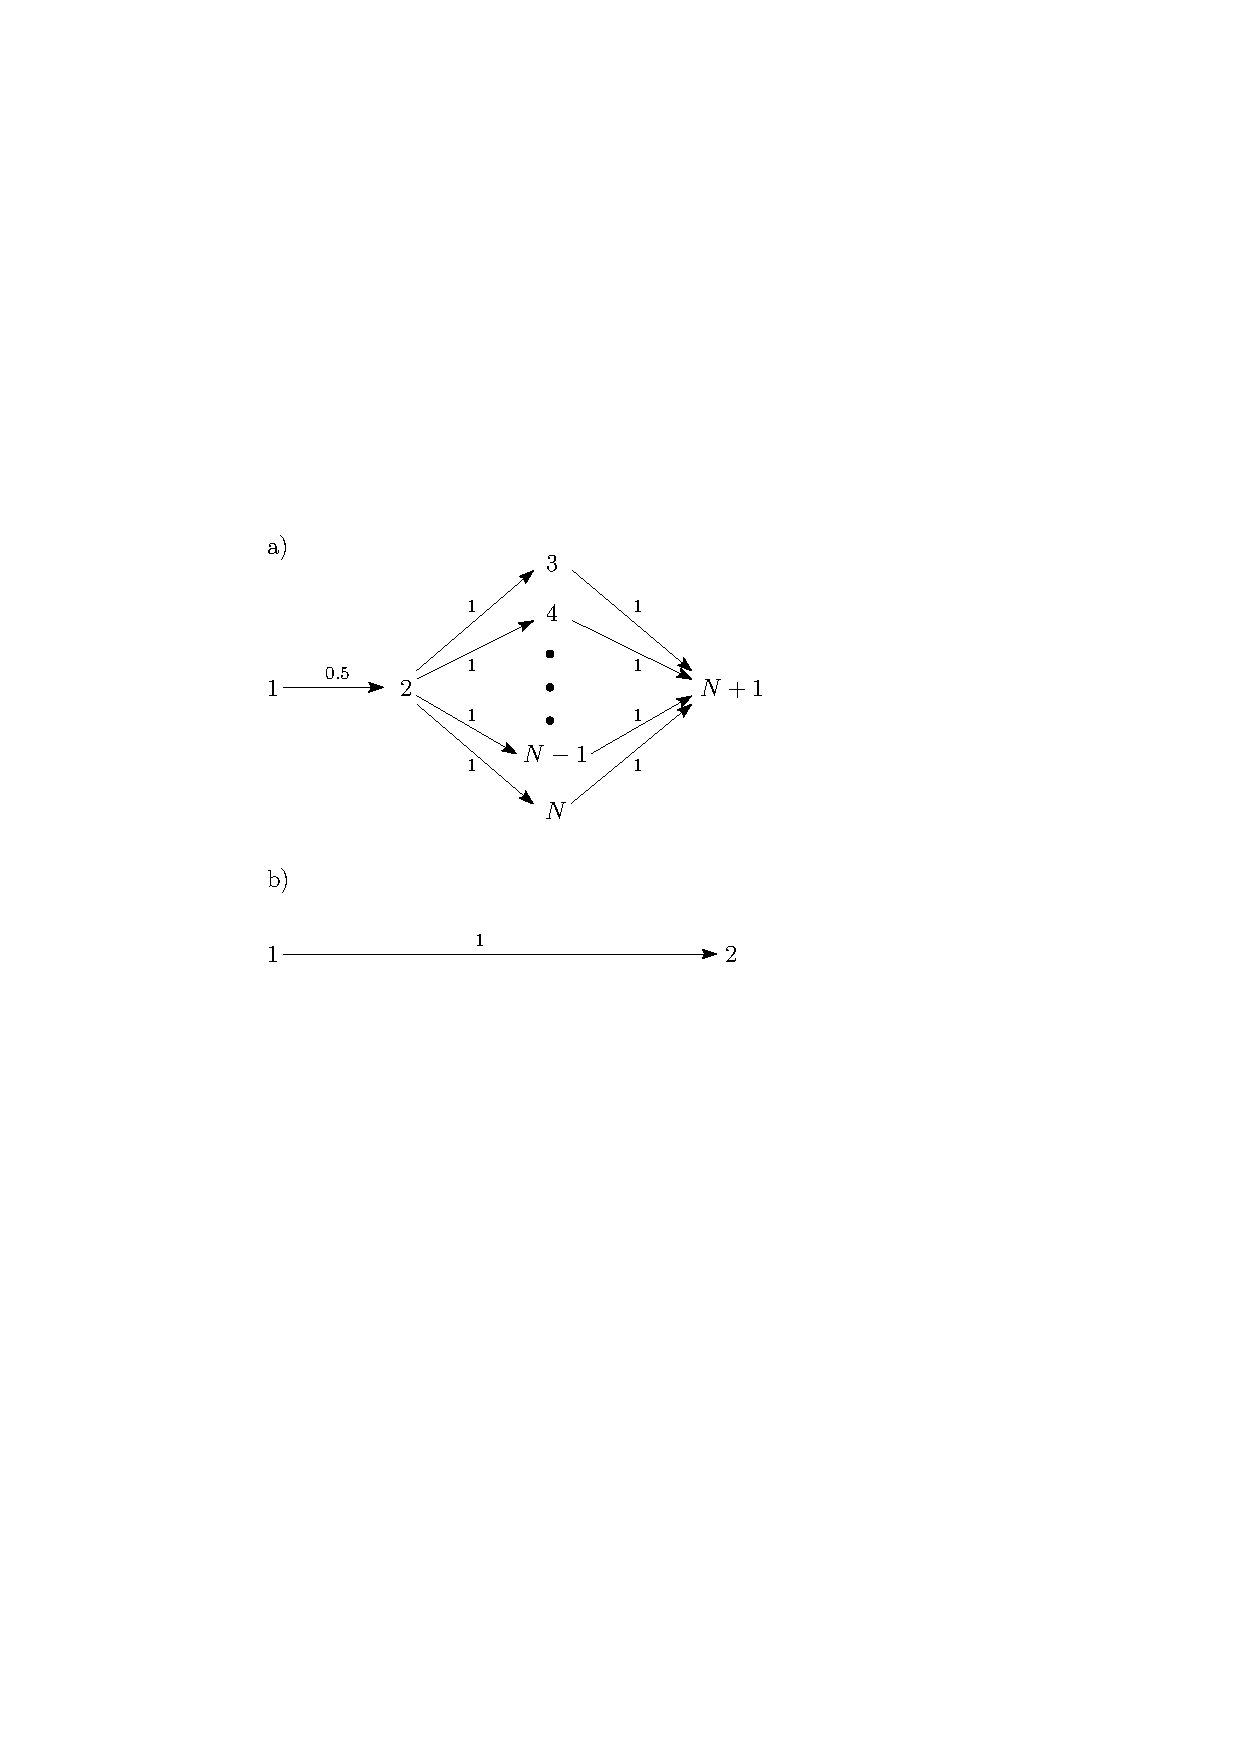
\includegraphics[width=0.5\columnwidth]{extremeexample.pdf}
% }
% \caption{An extreme example on the difference between the expected number of successful paths and the probability of reaching the destination.
% Figure a) shows a network consisting of $N+1$ states, where all transfer probabilities are equal to one except $p_{12} = 0.5$.
% The expected number of successful paths from state $1$ to state $N+1$ is given by $h_1 = 0.5(N-2)$ and the 
% probability of reaching state $N+1$ from state $1$ equals $0.5$. That is, while $h_1$ increases linearly with $N$,
% the probability is independent of $N$.
% This difference is explained by the fact that all paths from $1$ to $N+1$ are overlapping and 
% their success depends only on the success of the transfer from $1$ to $2$. 
% Figure b) shows a simple network in which $h_1=1$. Thus, if $N > 4$, the expected number of successful paths
% in case a) is greater than in case b), even though the probability of reaching the destination is greater in b).
% }
% \label{aariesimerkki}
% \end{figure}
% 
% In Figure \ref{aariesimerkki}, an extreme example on the differences between the two studied reliability measures is presented.
% Calculating the expected number of successful paths in the network shown in Figure \ref{aariesimerkki}a produces an overoptimistic estimate of 
% the reliability of the path. The difference is explained by overlapping, that is, the success of the journey depends only on the success of a single bottleneck.
% 
% \begin{figure*}
% \centering{
% 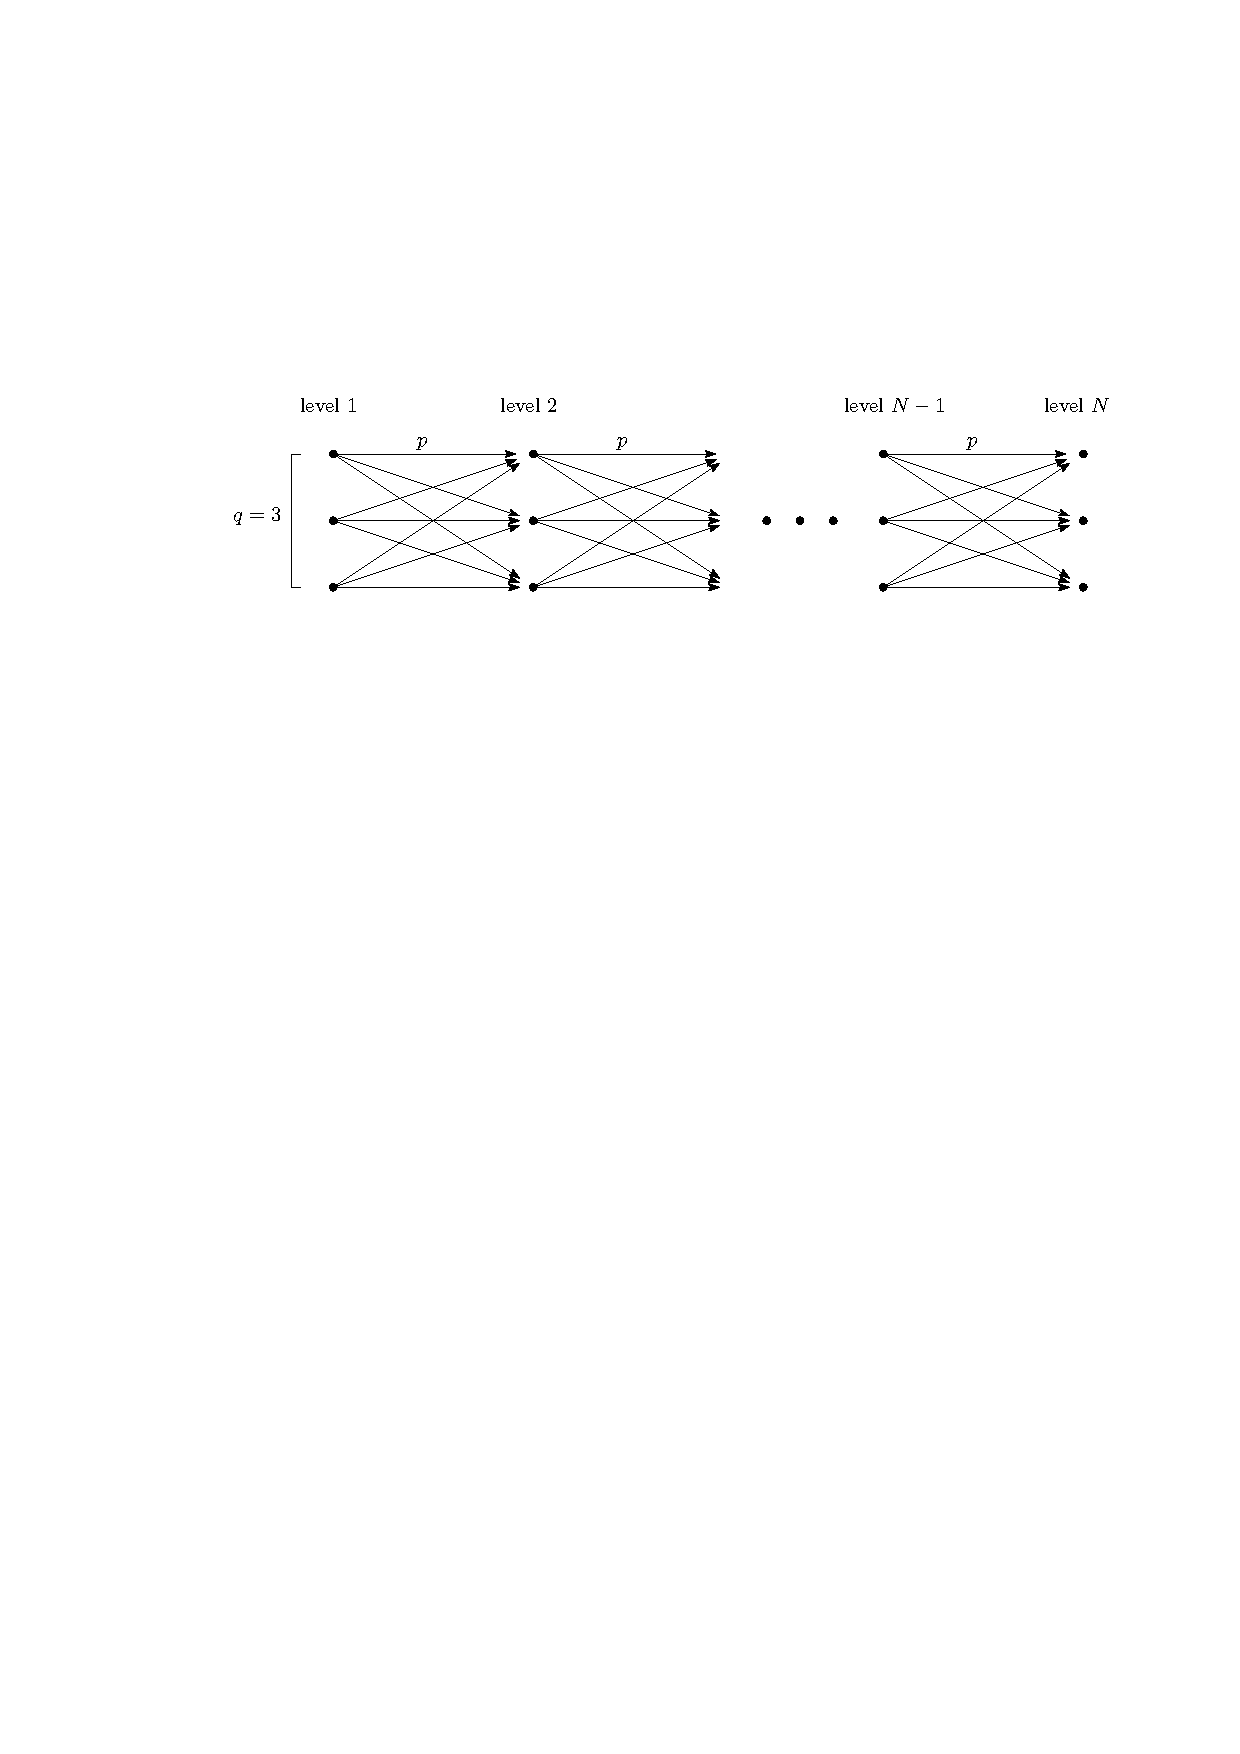
\includegraphics[width=0.8\columnwidth]{numerical01c.pdf}
% }
% \caption{An example on the difference between the expected number of successful paths and the probability of reaching the destination in
% regular networks.
% The figure shows the structure of the regular network consisting of $N$ levels, each of which consists of $q=3$ states. 
% The transition probability from each state on level $L$ to each state on level $L+1$ equals $p$. The probability of a successful journey from level $1$ to level $N$
% equals $(1-(1-p)^q)^{N-1}$. The expected number of successful paths from level $1$ to level $N$ is given by $(qp)^{N-1}$.
% }
% \label{regularesimerkki}
% \end{figure*}
% 
% Figure \ref{regularesimerkki} shows an example of a regular network consisting of $N$ levels, each of which consists of $q$ states. 
% The transition probability from each state on level $L$ to each state on level $L+1$ equals $p$. Clearly, the probability of 
% a successful transfer to the next level is given by $1-(1-p)^q$ and thus, the probability of a successful journey from level $1$ to level $N$
% equals ${(1-(1-p)^q)^{N-1}}$. The expected number of successful paths from each state on level $N-1$ to a state on level $N$ equals $qp$.
% Moreover, since the expected number of successful paths $h_L$ from a state on level $L$ to a state on level $N$ satisfies 
% $h_L = qp h_{L+1}$, we have $h_1 = (qp)^{N-1}$. Note that if $qp < 1$, both measures decrease exponentially with respect to the 
% number of transfers $N-1$, and if $q=1$, the two measures coincide.
 





\section{Numerical experiments}
\label{experiments}
In the following, computational results obtained by backward induction are presented. 
The transfer probabilities between legs are determined by assuming 
gamma distributed ride times similarly as in 
\cite{russell, chiang}. 
More precisely, given the expected ride time $t_i$ of leg $i$, we define the 
ride time $\tau_{i}$ as a random variable $\tau_{i} \sim \text{Gamma}( \alpha t_{i}, \beta , \delta t_{i} )$,
where the $\text{Gamma}( \alpha, \beta , \delta )$ distribution is defined by the 
probability density function 
\begin{align}
\label{gammakaava}
f(x)=\frac{(x-\delta)^{\alpha-1} e^{-(x-\delta)/\beta}}{\beta^{\alpha} \Gamma (\alpha)} \ \ \ \mbox{ for } x > \delta \geq 0.
\end{align}
The numerical examples are restricted to calculating the the expected number of feasible paths and 
the probability of reaching the destination during a pre-defined time horizon. However, a general objective function
defined as a combination of expected waiting time, number of transfers, expected ride time, expected walking time and reliability
is incorporated with minimal effort (see Equation (6) in \ref{jtoits}).


\subsection{Description of instances}
\label{reallife}
The Helsinki tram network consists of ten tram lines, operated by 50 trams, and 154 stops. 
The tram schedules of Helsinki Region Transport are available at \cite{reittiopas} and
the instances are available at \verb=http://math.tkk.fi/%7elehame/dju=.

In each instance, the origin and destination nodes $v_o$ and $v_d$ are chosen randomly from the 
set of $154$ tram stops, see Figure \ref{verkot01}. 
The departure time is set equal to 9:00 and the length of the time horizon
is defined by $T = 1.6 d(v_o,v_d)$, where $d(v_o,v_d)$ is the expected duration of the shortest path from $v_o$ to $v_d$ 
in the tram network.
Each (tram) service $k$ operating within the time horizon is determined by a \emph{scheduled route} extracted from the timetables, that is, 
a sequence $((v_0^k,t_0^k),\ldots,(v_p^k,t_p^k))$ of 
nodes, where $t_i^k$ is the expected passing time at node $v_i^k$ 
for $i=0,\ldots,p$. Each service is
decomposed as a set of legs.

\begin{figure}[ht]
\begin{center}
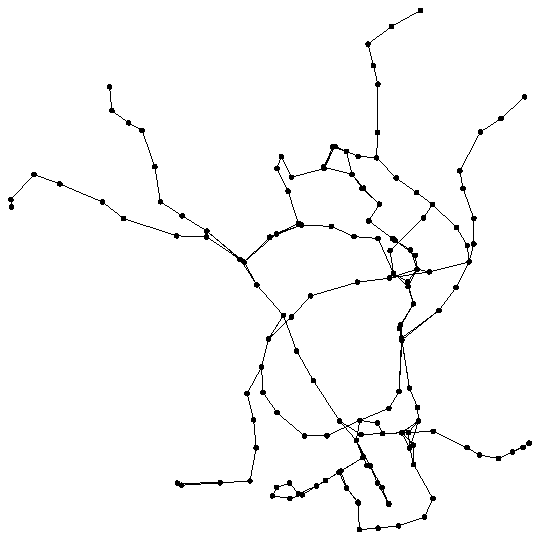
\includegraphics[width=0.6\columnwidth]{verkot01a}
\end{center}
\caption{The tram network of Helsinki consisting of ten tram lines and 154 stops. 
}
\label{verkot01}
\end{figure}

% By means of the above procedure, ten instances were generated. 
% The file names of the instances are of the form 'b$x$.dat', where $x \in \{1,\ldots,10\}$.
% Each row in the files corresponds to a leg. The first and last row in each file correspond to the origin and destination leg, respectively 
% (see Section \ref{problem}). The five columns denote the expected start and end time (in minutes), 
% the start and end node and the service number, respectively. 

\subsection{Results}

\begin{table}[ht] 
\caption{ Computational results. The table shows the probability $V(1)$ of reaching the destination 
leg $n$ from
the origin leg $1$, the expected number of successful paths $h_1$ from $1$ to $n$ and the corresponding 
computation times in seconds.}
\centering     
{\scriptsize
\begin{tabular}{|c|cc|cc|}
\hline 
\multirow{2}{*}{Instance} & \multicolumn{2}{|c|}{Probability} & \multicolumn{2}{|c|}{Exp. number of paths} \\
\cline{2-5}
& CPU time (s) & $V(1)$ & CPU time (s) & $h_1$ \\
\hline 
 \text{b1} & 0.23 & 0.97 & 0.15 & 106.88 \\
 \text{b2} & 0.06 & 1. & 0.04 & 42.31 \\
 \text{b3} & 0.06 & 1. & 0.04 & 20.72 \\
 \text{b4} & 0.06 & 0.46 & 0.04 & 1.25 \\
 \text{b5} & 0.31 & 0.97 & 0.22 & 7.05 \\
 \text{b6} & 0.1 & 0.91 & 0.07 & 2.67 \\
 \text{b7} & 0.09 & 0.85 & 0.06 & 12.72 \\
 \text{b8} & 0.05 & 0.7 & 0.03 & 0.7 \\
 \text{b9} & 0.12 & 0.99 & 0.08 & 25.67 \\
 \text{b10} & 0.08 & 0.79 & 0.06 & 83.34 \\
 \hline
\end{tabular}
}
\label{tulokset01a}
\end{table}


The computational results of ten instances are shown in Table \ref{tulokset01a}.
For each instance the name, the 
probability $V(1)$ of reaching the destination during the time horizon, the expected number of successful paths $h_1$,
and their respective computation times are given.
%The first column shows the name of the instance. The third and fifth columns show the 
%probability $V(1)$ of reaching the destination and the expected number of successful paths $h_1$. 
%The second and fourth columns show the corresponding computation times.
By looking at the computation times, we see that 
all instances were solved within a fraction of a second. In addition, calculating the expected 
number of successful paths is slightly faster than calculating probability, which involves sorting.

Since the expected number of successful paths represents the number of alternatives,
even a large value of $h_1$ does not guarantee that the destination will be reached in time (b10).
On the other hand, small values of $h_1$ seem to correspond to small probabilities (b4 and b8).
For instances b2 and b3 with $V(1)=1$, the expected number of successful paths gives additional
information: Instance b2 provides more alternative routes for the commuter than b3.   



\chapter{Economic equilibrium}
\label{economicmodels}
\ref{ccompejor} introduces a stochastic network model to characterize the 
behavior of customers and transport operators in a demand-responsive transport market. 
Customers seek rides to minimize travel time and transport operators aim to maximize profit. 
Demand-responsive transport is considered as a complementary service to conventional public transport services and 
customers are assumed to choose the utility-maximizing alternative from the available transport modes.
An \emph{economic equilibrium} is defined as a state in which the demand meets the supply of trips: 
the choices of transport operators
do not change if the demand remains constant and the choices of customers
do not change if the supply of trips remains constant. 

This approach is somewhat similar to the taxi model proposed in \cite{yang2010}. The main difference is that in a taxi service, 
customers are delivered to their destinations directly, whereas in a demand-responsive transport service, a vehicle can serve several customers 
simultaneously and therefore a customer's trip from an origin to a destination is not necessarily a direct one. 
In other words, the route of a taxi is determined by two points (origin and destination), but 
demand-responsive transport routes may include several stops, similarly as bus routes. 


The stochastic model for demand-responsive transport is governed by the following preliminary assumptions.
\begin{enumerate}
\item
There are $N$ vehicles that produce trips between 
origins and destinations in a specific operating zone. 
Different trips may have different prices and
travel times. A single vehicle can simultaneously serve several customers.
\item
The subjective price of a trip is defined as a combination of ticket price and travel time.
Customers choose between trips provided by 
DRT and a virtual mode\footnote{The virtual mode represents alternatives for the DRT service.} by comparing the subjective 
prices of different trips.
\end{enumerate} 

%The following sections present a Markov
%Sections \ref{demand} and \ref{vehiclemovements} discuss the demand and supply models in more detail.
%Sections \ref{compdescription} and \ref{monopdescription} present two different market models for demand-responsive transport.

\section{Demand}
\label{demand}
Let us consider a set of \emph{nodes} $I$ representing the origins and destinations of customers in a specific operating zone.
Each pair of nodes $(i,j) \in I \times I$ is associated with a specific \emph{direct ride time} $t_{ij}$.

A \emph{trip} from an origin $i_0 \in I$ to a destination $i_d \in I$ is defined as an acyclic sequence of nodes 
$(i_0,i_1,\ldots,i_{d-1},i_d)$ in $I$.
When a customer takes a trip $(i_0,i_1,\ldots,i_{d-1},i_d)$, the customer enters a vehicle at $i_0$, which
visits the nodes $i_1,\ldots,i_{d-1}$ before the drop-off of the customer at $i_d$. That is, the
trip denotes the path of the vehicle that transports the customer from $i_0$ to $i_d$.
For example, a \emph{direct} trip from $i_0 \in I$ to $i_d \in I$, denoted by $(i_0,i_d)$, describes a trip in which a customer enters 
a vehicle at $i_0$ and the vehicle drives directly to $i_d$ without stopping between $i_0$ and $i_d$. 

Each trip $r$ has a specific ticket price $p_r$. 
Note that the prices of trips with the same origin and destination may be different.
Each customer seeks a trip to minimize the \emph{subjective price} $g_r^{\rm DRT}$, 
defined as a combination of ticket price $p_r$ and \emph{travel time} $t_{r}^{\rm DRT}$, that is,
\begin{align}
\label{asiakashinta}
g_{r}^{\rm DRT} = p_{r} + \beta t_{r}^{\rm DRT},
\end{align}
where $p_{r}$ is the ticket price for the trip $r$ and $\beta$ is the customers' 
monetary value of unit travel time.

The choices of customers are determined by a logit model as follows.
The subjective trip price of a trip from $i$ to $j$ provided by the virtual mode is denoted by $\bar{g}_{ij}$.
The probability that a customer traveling from $i$ to $j$ chooses a DRT trip $r \in \mathcal{R}_{ij}$, where $\mathcal{R}_{ij}$ denotes the 
set of trips from $i$ to $j$, is defined by
\begin{align}
\label{kysyntatn}
P_{r}^{\rm DRT} = 
\frac{\exp(-\theta g_{r}^{\rm DRT})}{\exp(-\theta \bar{g}_{ij}) + \sum_{r' \in \mathcal{R}_{ij}}\exp(-\theta g_{r'}^{\rm DRT})},
\end{align}
where $\theta$ is a nonnegative parameter describing the uncertainty in transport services and demand
from the perspective of customers.  
Clearly, the above logit model has the property of independence from irrelevant alternatives, that is, 
the ratio $P_{r}/P_{r'}$ depends on the subjective prices of trips $r$ and $r'$ but
not on the subjective prices of other trips \citep{small2007}.

The expected demand for a trip $r \in \mathcal{R}_{ij}$ is given by
%\begin{align}
%\label{matkakysynta}
$Q_{r}^{\rm DRT} = Q_{ij} P_{r}^{\rm DRT},$
%\end{align}
where $Q_{ij}$ denotes the total demand from $i$ to $j$, including the demand $Q_{ij}^{DRT}$ for DRT and the demand for the virtual mode.

\section{Supply}
\label{vehiclemovements}
We assume that there are $N$ vehicles available for transporting customers. 
At any point in time, each vehicle follows a specific route $(i_0,i_1,\ldots,i_m)$ 
determined by a sequence of nodes in the transportation network.
The vehicle starts at the first node $i_0$ and proceeds by visiting the other nodes $i_k$
for $k=1,\ldots,m$ in the order determined by the route.
Each node corresponds to a stop during which customers may enter or exit the vehicle.

During the execution of the route $(i_0,i_1,\ldots,i_m)$, the vehicle produces
trips that are subsequences of $(i_0,\ldots, i_m)$. This idea of producing trips 
is in fact similar as in traditional public transport: a bus with a given route 
produces trips that are subsequences of the route.

The \emph{state} of a vehicle describes which part of the route the vehicle is currently executing.
Each time a vehicle following a route $(i_0,\ldots,i_m)$ arrives at stop $i_k$, 
we say that the vehicle \emph{transfers} to a new state.
Similarly as routes, the states are defined as sequences of nodes.
The difference between states and routes
is that the state of a vehicle corresponds to the \emph{remaining part} of its current route. 
That is, the vehicle transfers to a new state each time it arrives at a stop, even if the route remains unchanged.
During the execution of a route $(i_0,\ldots,i_m)$, the vehicle successively transfers to states 
$(i_0,\ldots,i_m),(i_1,\ldots,i_m),(i_2,\ldots,i_m),\ldots,(i_{m-1},i_m)$.


\section{Competitive market}
\label{compdescription}
Most existing demand-responsive transport services provide door-to-door transportation for elderly or handicapped people
and require customers to book trips at least one hour in advance \citep{cordeau05,jouko}.
Conventionally, the trips are organized centrally via \emph{travel dispatch centers}, which have the capability of
assigning customers to vehicles and optimizing the routes \citep{mageean}.
In contrast to such centralized services, \ref{ccompejor} considers a competitive form of demand-responsive transport in which 
each driver providing service attempts to maximize his/her profit. That is,
the movement of vehicles is governed by the decisions of individual drivers, 
instead of a travel dispatch center controlled by a single transport operator.
This market structure is in fact similar to conventional taxi-markets, which have been extensively studied, see for example 
\citep{hackner1995,arnott1996,cairns1996,flores-guri2003,lagos2003,wong2005,matsushima2006,fernandez2006,moore2006,yang2002,yang2005,yang2010}.

In a competitive market, the drivers attempt to transfer to
states at which the \emph{expected profit rate} is maximized. 

By assuming a logit model similar to the one in Equation \eqref{kysyntatn},
the probability that a vehicle at state $s$ transfers to state $s' \in \mathcal{S}$
is given by
\begin{align}
\label{transitionprobability}
P_{s,s'} = 
\left\{
\begin{array}{llr}
\frac{\exp(\theta^d U(s'))}{\sum_{s'' \in \mathcal{S}_{s}} \exp(\theta^d U_{s''})}, 
& \mbox{if } s' \in \mathcal{S}_s & (\mathcal{S}_s = \mbox{ successor set of $s$)}, \\
0 & \mbox{otherwise},&
\end{array}
\right.
\end{align}
where $\theta^d$ is a 
nonnegative parameter reflecting the uncertainty on
demand and DRT services from the perspective of drivers, $U(s)$ is the expected profit rate at state $s$ and 
$\mathcal{S}_s$ is the set of states to which a transfer from state $s$ is possible. 


\subsection{Network equilibrium}
\label{networkequilibrium}
The drivers attempt to maximize profit rate by 
transporting as many customers per unit time as possible. Thus, we expect that the
drivers prefer detours instead of direct routes in order to serve more 
customers.
In some cases, however, producing only direct trips may be more profitable. 

We also expect that the customers prefer direct trips instead of detours.
However, if many vehicles produce non-direct trips, 
the travel times in non-direct trips may be smaller than in direct trips due 
to small waiting times.

The movement of vehicles is described by means of the \emph{arrival rates}
of vehicles at different states and
the movement of customers is described by means of the demands 
for different DRT trips. 
A \emph{network equilibrium} denotes a situation in which the arrival rates at states and demands for different trips meet.
% 
% the following combination of
% arrival rates $T_s^*$ at states $s \in \mathcal{S}$ and demands $Q_r^{{\rm DRT}*}$ for trips $r \in \mathcal{R}$: 
% \begin{itemize}
% \item
% The set of arrival rates $\{T_{s_1}^*,\ldots,T_{s_{|\mathcal{S}|}}^*\}$ of vehicles at states $s_i \in \mathcal{S}$ 
% generates the set of demands $\{Q_{r_1}^{{\rm DRT}*},\ldots,Q_{r_{|\mathcal{R}|}}^{{\rm DRT}*}\}$ for trips $r_i \in \mathcal{R}$.
% \item
% The set of demands $\{Q_{r_1}^{{\rm DRT}*},\ldots,Q_{r_{|\mathcal{R}|}}^{{\rm DRT}*}\}$ for trips $r_i \in \mathcal{R}$
% generates the set of arrival rates $\{T_{s_1}^*,\ldots,T_{s_{|\mathcal{S}|}}^*\}$ of vehicles at states $s_i \in \mathcal{S}$. 
% \end{itemize}
By using Brouwer's fixed point theorem, the following result is obtained.

\begin{theorem}
For any finite transportation network, there exists a network equilibrium.
\end{theorem}


%\subsection{Algorithm}
%\label{ratkaisu01}
The idea for finding a network equilibrium is to solve 
both the customer choice subproblem and the vehicle movement subproblem iteratively 
until a convergence criterion is met, similarly as in \citep{yang2010}. 
% The outline of the procedure is presented in Algorithm \ref{compalg}.
% 
% \begin{algorithm}[H]
% \begin{algorithmic}
% \STATE \emph{Input}: Set $I$ of nodes, direct ride time $t_{ij}$, cost $c_{ij}$, demand $Q_{ij}$,
% ticket price $p_{r}$, cost of virtual mode $\bar{g}_{ij}$ 
% for all pairs $i,j \in I$ of nodes, number of vehicles $N$, 
% customers' monetary value for unit time $\beta$
% and the uncertainty parameters $\theta,\theta^d$.
% \STATE \emph{Output}: Equilibrium arrival rates $T_s$ of 
% vehicles at states $s \in \mathcal{S}$.
% \STATE Initialize the arrival rates $T_s$ of vehicles by dividing the vehicles
% evenly among all states $s \in \mathcal{S}$, $T_{s} = \frac {N}{d_s |\mathcal{S}|}$; 
% \REPEAT
% \STATE \textbf{Customer demand updating:} Calculate $Q_{r}^{\rm DRT}$ for all 
% $r \in \mathcal{R}$;
% \STATE \textbf{Vehicle movements:} Solve $T_s$ for all $s \in \mathcal{S}$;
% \UNTIL{convergence}
% \end{algorithmic}
% \caption{Equilibration of DRT.}
% \label{compalg}
% \end{algorithm}

%\section{Numerical examples}
\subsection{A three node example}
\label{compexample}
Let us demonstrate the calculation of the competitive network equilibrium in a simple case 
in which the network consists of three nodes denoted by $1,2,3$, as shown in Figure \ref{3node01}. 
The set of states consists of the 12 possible sequences of two and three nodes. 
In large networks, one might want to
limit the number of states by including only a part of all 
possible sequences, since the number of possible sequences of $n$ nodes equals $n!$. 

\begin{figure}[ht]
\begin{center}
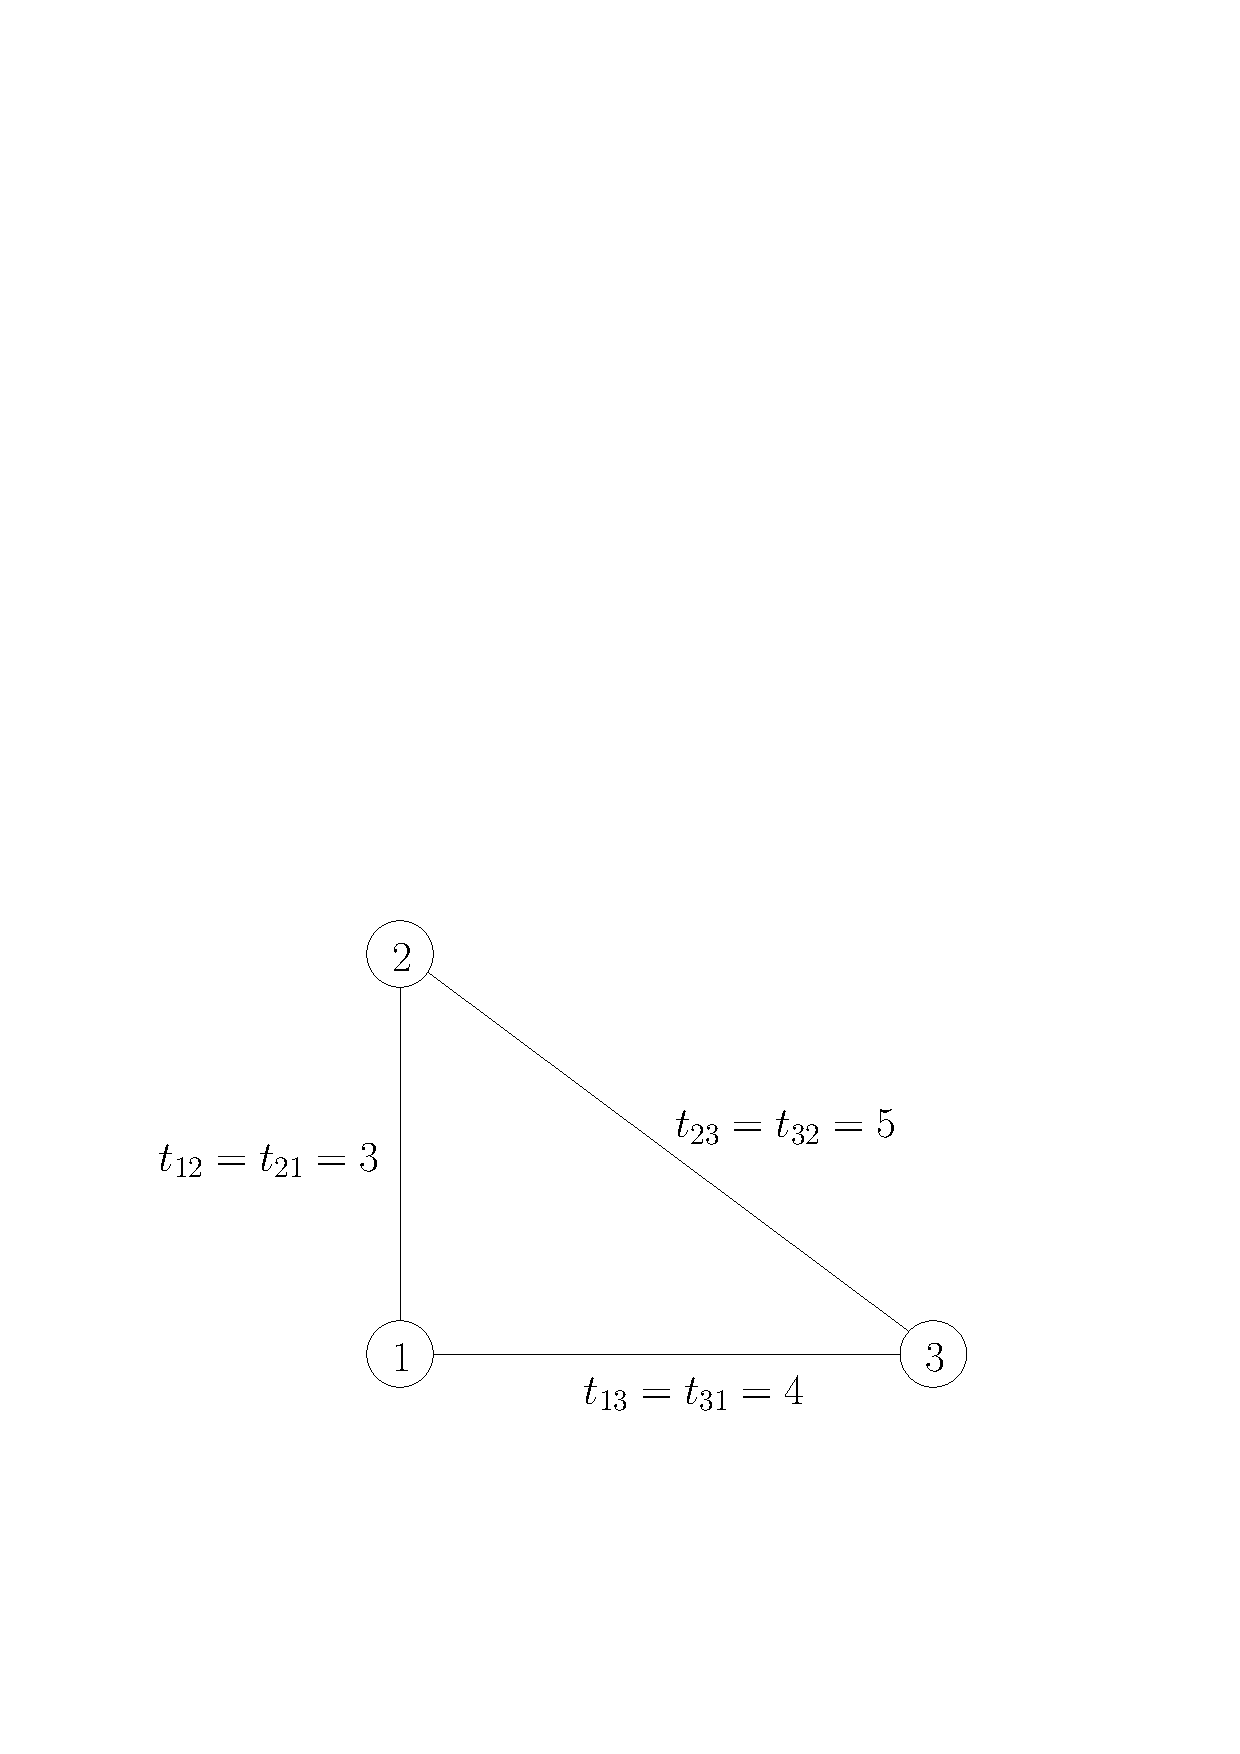
\includegraphics[width=0.6\columnwidth]{3node01}
\caption{A three node example network. The distances between the nodes 
(in kilometers) are equal to the direct ride times $t_{ij}$.}
\label{3node01}
\end{center}
\end{figure}

The solid lines in Figure \ref{convergence01} show the
arrival rates $T_s$ of vehicles at different states $s \in \mathcal{S}$ after each step of the equilibration algorithm. 
The black and grey dashed lines show on a logarithmic scale 
the convergence of the arrival rate vector $T$ and the demand vector $Q^{\rm DRT}$, respectively.

\begin{figure}[ht]
\begin{center}
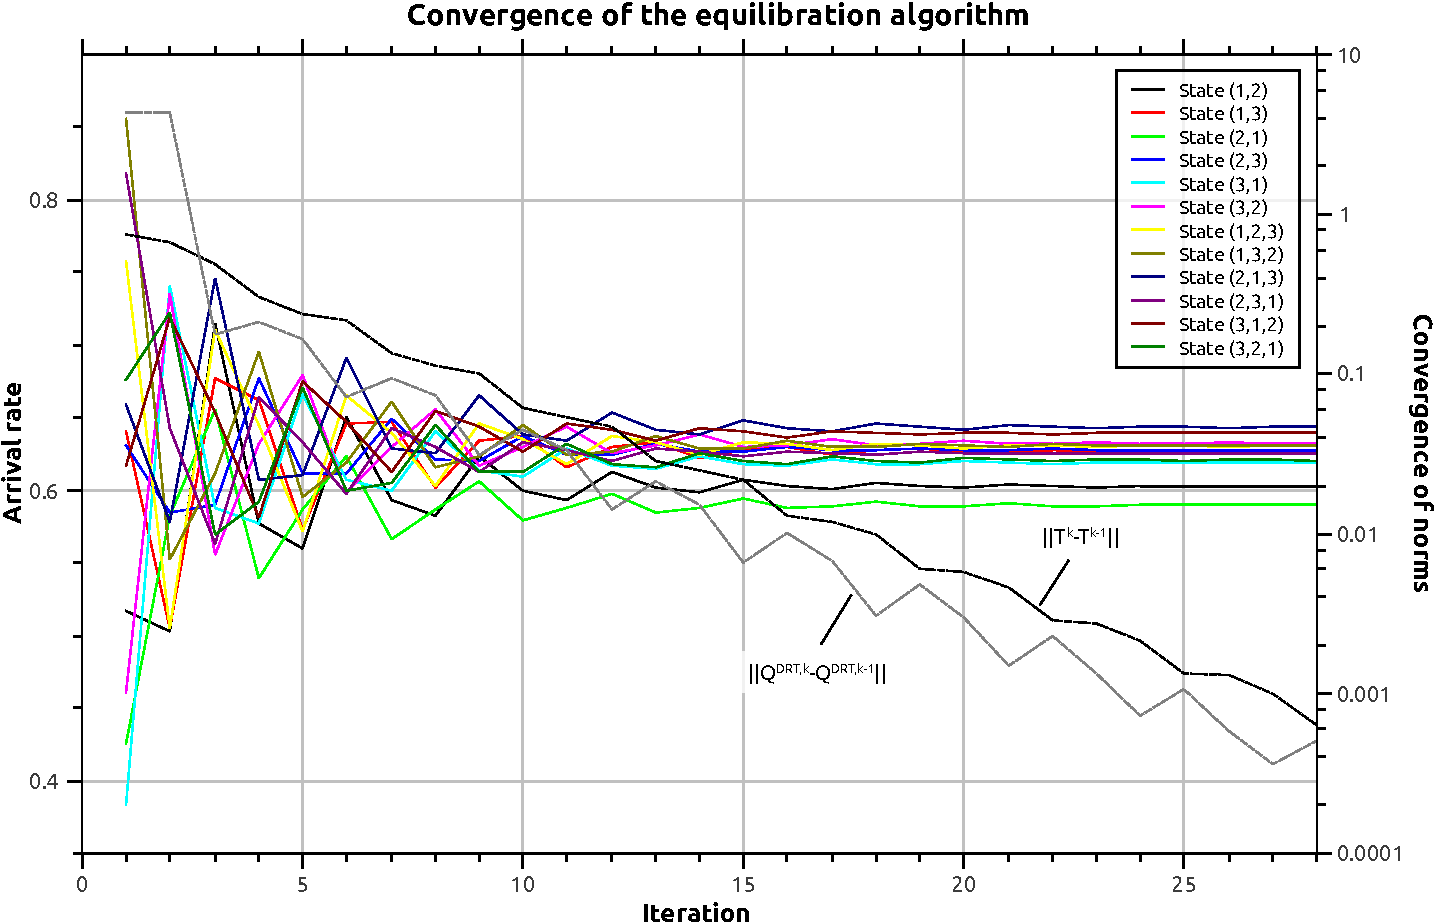
\includegraphics[width=0.9\columnwidth]{convergence01}
{\tiny
\begin{tabular}{|c|cccccccccccc|}
\multicolumn{13}{c}{} \\
\hline
\multicolumn{13}{|c|}{Arrival rates at states in the network equilibrium $T^*$} \\
\hline
State $s$ & (1,2) & (1,3) & (2,1) & (2,3) & (3,1) & (3,2) & (1,2,3) & (1,3,2) & (2,1,3) & (2,3,1) & (3,1,2) & (3,2,1) \\
\hline
Arrival rate $T_s$ & 0.603 & 0.627 & 0.590 & 0.628 & 0.619 & 0.632 & 0.631 & 0.631 & 0.644 & 0.626 & 0.639 & 0.621 \\
\hline
\end{tabular}
}
\caption{Convergence of the equilibration algorithm in the three node example. The solid lines in show the
arrival rates $T_s$ of vehicles at different states $s \in \mathcal{S}$ after each step of the algorithm. 
The black and grey dashed lines show on a logarithmic scale 
the convergence of the arrival rate vector $T$ and the demand vector $Q^{\rm DRT}$, respectively.
The network equilibrium is defined by the
arrival rates at different states shown in the table below the figure.}
\label{convergence01}
\end{center}
\end{figure}

By looking at the solid lines, we see the oscillatory nature of the arrival rates: When the
arrival rate of vehicles in a specific state $s$ increases during the equilibration, the number 
of customers available for a single vehicle in that state decreases. 
This causes the drivers to choose other states instead of $s$.
When the arrival rate at state $s$ decreases, it becomes more profitable for individual vehicles
and results in drivers choosing state $s$ more often. In the network equilibrium, the arrival rate is highest
at state $(2,1,3)$ and lowest at state $(2,1)$.

Referring to the dashed lines, which are roughly straight lines on a logarithmic scale, 
we see that the norms of the arrival rate and demand vectors converge exponentially
with respect to the number of iterations. 

% Decreasing the difference $\|T^k -T^{k-1}\|$ by a factor of $F \in \mathbb{R}$
% requires $G \in \mathbb{N}$ iterations. That is, $\|T^k -T^{k-1}\| = \frac{1}{F^K} \|T^{k-GK} -T^{k-1-GK}\|$
% for $K \in \mathbb{N}$.
% By looking at the slope of the dark dashed line, we see that the 
% difference $\|T^k -T^{k-1}\|$ decreases 
% by a factor of $10$ in approximately $10$ iterations, that is, $\|T^k -T^{k-1}\| = \frac {1}{10^K} \|T^{k-10K} -T^{k-1-10K}\|$
% for $K \in \mathbb{N}$.

\subsection{Long-run example}
\label{longrun}
In an unregulated demand-responsive transport service operated by a single operator, 
we expect that the number of vehicles and ticket price are chosen in a way that
the total profit rate is maximized in the long run.
In a competitive demand-responsive market with no entry limits, 
we expect that the number of vehicles increases as long as the profit
rate of vehicles is positive. 
Regulating the number of vehicles and ticket price could improve the service
from the customers' point of view as well as from the perspective of transport operators.
In the following, we study different characteristics of demand-responsive transport
as a function of the number of vehicles $N$ and average price per kilometer $p$.
The network equilibrium was calculated for different numbers
of vehicles $N$ and prices per kilometer $p$.
For each combination of $N$ and $p$, the total profit rate, profit 
rate per vehicle and customer surplus\footnote{\emph{Customer surplus} is defined
as the difference between the subjective price of the virtual mode and 
the subjective price of DRT ,namely, by
$
\sum_{(i,j) \in I \times I} \sum_{r \in \mathcal{R}_{ij}} Q^{DRT}_r  (\bar{g}_{ij}-g_r),
$
where $Q^{DRT}_{ij}$ is the total demand for DRT trips from $i$ to $j$,
$Q_{ij} - Q^{DRT}_{ij}$ is the demand for the virtual mode from $i$ to $j$, $\mathcal{R}_{ij}$
is the set of DRT trips from $i$ to $j$, $g_r$ is the subjective price
of trip $r$ and $\bar{g}_{ij}$ is the subjective price of the virtual mode from $i$ to $j$.} 
were calculated. The results are shown in Figure \ref{a-equilibria01}.

\begin{figure}[ht]
\begin{center}
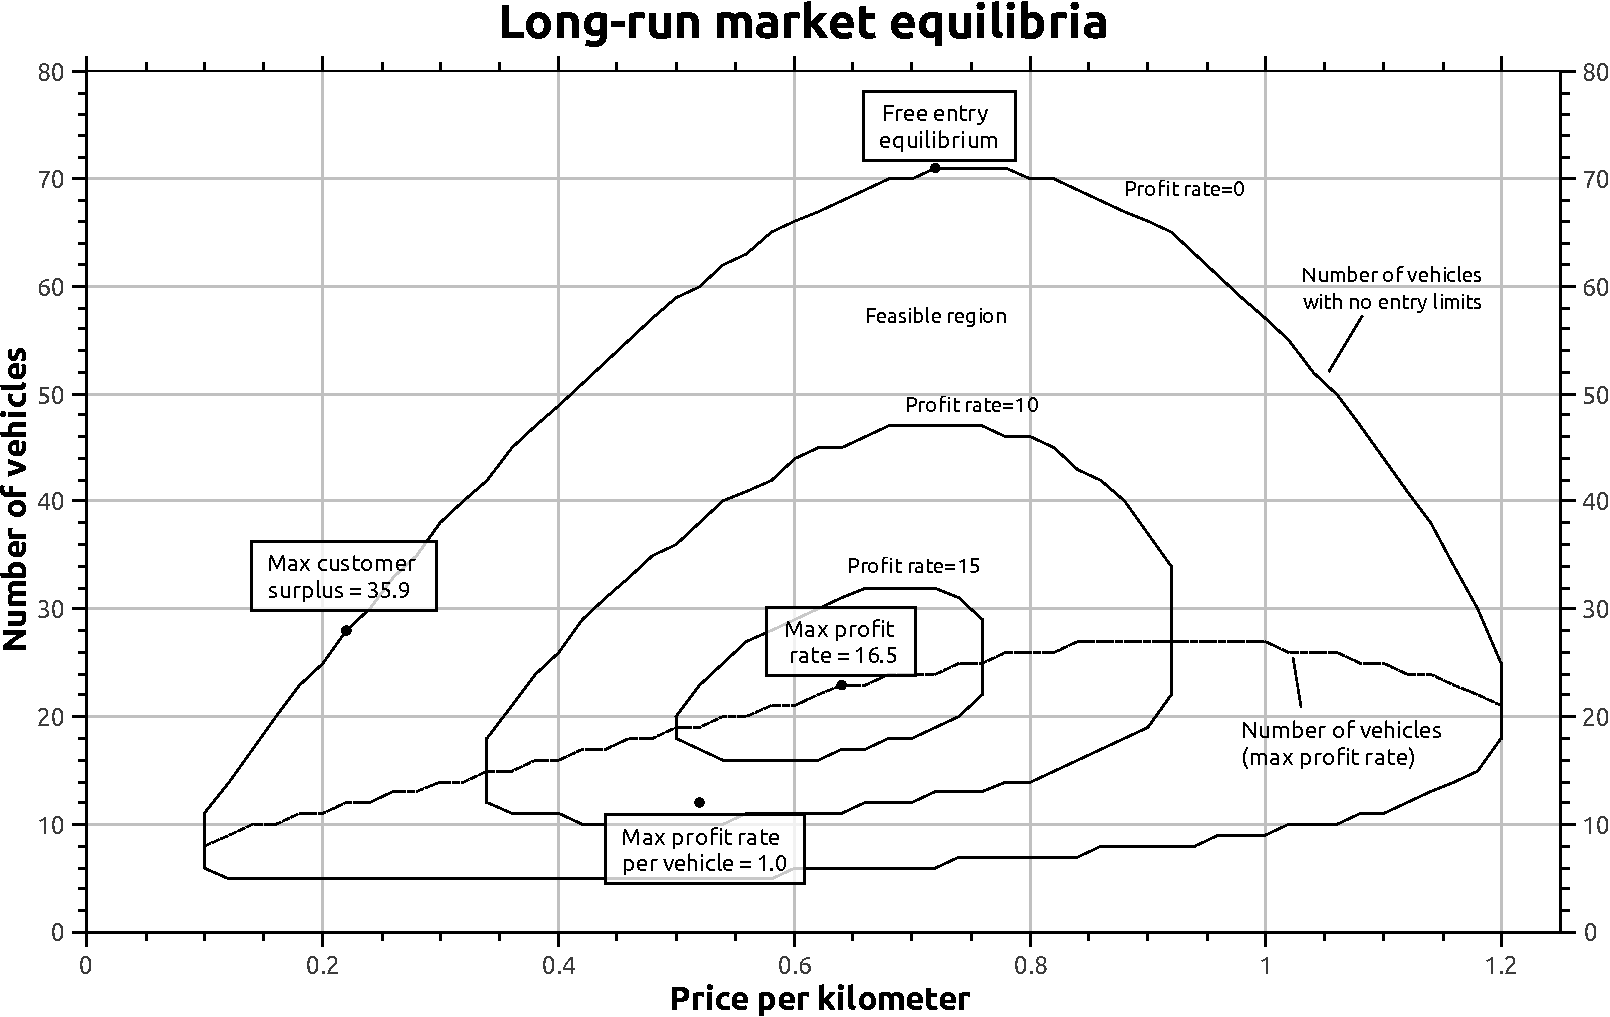
\includegraphics[width=0.9\columnwidth]{a-equilibria01}
\\
{\scriptsize
\begin{tabular}{|p{2.0cm}|p{1.0cm}|p{1.0cm}|p{1.5cm}|p{1.4cm}|p{1.2cm}|p{0.75cm}|p{0.9cm}|}
\multicolumn{8}{c}{} \\
\hline
Equilibrium & Number of vehicles & price per kilometer & Demand for DRT (customers/min) & 
Tot. profit rate / per vehicle (EUR/min) & Surplus (EUR/min) & Travel time ratio & Average occupancy \\
\hline
Max. customer surplus & 28 & 0.22 & 16.1 & 0.13 / 0.005 & 35.9 & 1.24 & 2.4 \\
\hline
Maximum total profit rate & 23 & 0.64 & 10.8 & 16.5 / 0.7 & 3.9 & 1.28 & 1.9 \\
\hline
Maximum profit rate per vehicle & 12 & 0.52 & 8.4 & 12.6 / 1.0 & 0.2 & 1.50 & 3.0 \\
\hline
Free entry equilibrium & 71 & 0.72 & 12.4 & 0.1 / 0.001 & 8.7 & 1.11 & 0.7 \\
\hline
\end{tabular}
}
\caption{Long-run market equilibria for the three node example. The first column shows the
four studied equilibrium points. The second and third columns show the 
number of vehicles and price per kilometer with which the equilibrium is achieved.
The remainder of the columns show the total demand for DRT, total profit rate and profit rate
per vehicle, customer surplus, the average ratio of travel time to direct travel time
and the average number of customers in a single vehicle.}
\label{a-equilibria01}
\end{center}
\end{figure}

The solid curves represent contour lines in which the total profit rate $U(N,p)$ of vehicles is equal ($=0,10,20$).
In particular, the outermost contour line corresponding to $U(N,p)=0$ encloses the 
\emph{feasible region}, that is, the area in which the service is profitable for drivers.
The dashed curve shows the number of vehicles for different prices for which
the total profit rate is maximized. The points represent the long-run market equilibria
defined in the previous section.

The table in Figure \ref{a-equilibria01} shows the demand for DRT, total profit rate, profit rate per vehicle, 
customer surplus, the average ratio of travel time to direct travel time
and the average number of customers in a single vehicle in the four equilibrium points.

By looking at the figure, we note that there is a significant difference between the
equilibria. In the free entry equilibrium, the number of vehicles is significantly
higher than in the other points. The average travel time ratio 
and the average occupancy are extremely low. This indicates that with no regulation, the
DRT service would approach a taxi-type service, in which all customers are 
transported privately and all trips are direct trips.

The difference in price between the free entry equilibrium and
the point in which the total profit rate is maximized is small. 
In addition, the number of served customers (demand for DRT)
is only slightly smaller in the maximum profit rate case compared to the free entry case.
However, maximizing the profit rate of vehicles would decrease the 
customer surplus and decrease the average level of service,
as can be seen by looking at the average travel time ratio and average occupancy.

The profit rate per vehicle is maximized with an extremely small number of vehicles.
In this case, only a small number of customers could be served and the level of service
would be poor.

The customer surplus is maximized by using a significantly
lower ticket price than would be optimal from the perspective of drivers. This is mainly due to the 
fact that the low price results in a high demand for DRT. Moreover, we note that the customer surplus
equilibrium is achieved by using price regulation exclusively. That is, the results suggest that 
the optimal solution from the customers' point of view would be to regulate price and allow free 
entry.

Reference \cite{kuhmostok} repeats the above example for a demand-responsive transport monopoly, where 
a single transport operator controls the transition probabilities of vehicles
between states, in contrast to the competitive market in which the routing decisions are made by individual drivers.
In this case, the matrix $P$ containing the transition probabilities $P_{s,s'}$ between states is referred to as a \emph{routing strategy} 
and the goal is to find a routing strategy that maximizes a given objective.

The results suggest that centralized routing strategies can be used to improve the efficiency of demand-responsive transport:
By maximizing profit by means of a centralized strategy, the total profit rate, demand and social welfare are increased from
the competitive equilibrium. The difference between the mechanisms is explained by the fact that in the competitive market, 
the routing decisions are based on the drivers' incomplete market information whereas in the case of a single transport operator,
the routing strategy is optimized by using information on the state of the entire network.



\chapter{Conclusions}
\label{conclusions}
This work presents mathematical models for demand-responsive transport and methods
that can be used to solve combinatorial problems related to vehicle routing and journey planning
in a transport network.

First,
we show how the demand for transportation can be satisfied by constructing routes for a fleet of vehicles,
assuming that the origins, destinations, and time limits of customers' trips are known.
Then, by considering a stochastic journey planning problem in a public transport network we determine
the optimal actions of commuters, assuming that the vehicle routes are fixed during a specific time horizon.
Finally, we present a stochastic network model
for determining the economic equilibrium in a transport network, that is, the point at which the demand meets the supply,
by assuming that commuters attempt to minimize travel time and transport operators aim to maximize profit.

The proposed models can be used to simulate the operations of public transport services ranging 
from paratransit services for the elderly and disabled to 
large-scale demand-responsive transport services. These calculations can 
provide valuable information to public authorities and planners of transportation services,
regarding, for example, regulation and investments.
The new methods for solving vehicle routing and journey planning problems can be 
used to improve the performance of different types of intelligent transportation systems and
to provide real-time travel information via mobile devices and electronic displays.
In addition to public transport, potential applications of the proposed algorithms
include freight transportation, courier and food delivery services, military logistics, and air traffic.

The main contributions to scientific methodology are summarized a follows.

The \emph{adaptive insertion algorithm} introduced in \ref{jeadarp} generalizes the insertion algorithm 
which is used to solve routing problems. The computational complexity of the adaptive algorithm can be controlled
smoothly, closing the gap between a greedy heuristic and complete enumeration.

\ref{jrbrorl} presents the \emph{routing by ranking} method, which connects recommendation-type 
link analysis to combinatorial path-finding problems. The idea is based on HITS, an eigenvector algorithm
originally developed for web information retrieval.

The \emph{maximum cluster algorithm} (\ref{jhitsdarpts}) is used to solve constrained routing problems with multiple vehicles by 
finding maximal sets of customers that can be assigned to a single vehicle. The article also 
introduces the \emph{clique detection method}, which finds a maximal set of customers, such that
no pair of customers in the set can be served by a single vehicle due to the constraints of the problem. 
This method is used to narrow down the search space and to detect infeasible problem instances.

\ref{jtoits} and \ref{jdjuejor} model the journey planning problem in a scheduled transport network as 
a Markov Decision Process (MDP). The \emph{actions} of the MDP are defined as \emph{preference orders} of possible 
alternatives in each part of the journey. 
The articles also show how the calculation of an optimal policy can be accelerated by assuming history independence and 
how the reliability of a journey is maximized by considering the \emph{expected number of successful paths} 
to the destination. In this context, a \emph{path} is defined as a sequence of scheduled legs in the transport network and for 
each pair $(i,j)$ of successive legs there is a specific transfer probability from $i$ to $j$.

\ref{ccompejor} introduces a stochastic network model for determining the 
economic equilibrium for demand-responsive transport. The existence of such an equilibrium is proved by using Brouwer's fixed point theorem. 
The model is used for optimizing fleet size and pricing as well as studying the effects of different regulation policies.

The following directions for future work are suggested:
%In its current form, routing by ranking seems to be an efficient method for finding feasible solutions to constrained routing problems with multiple vehicles. 
One could attempt to extend the routing by ranking algorithm to handle different types of cost functions. For example, the reliability 
of solutions could be optimized by defining travel times as random variables. The dynamic journey planning models could be enhanced 
by partitioning public transport stops into clusters, which would reduce the complexity of dynamic journey planning 
in large transport networks. Finally, the economic equilibrium model could be used to study the feasibility of demand-responsive transport
services in different types of real-life scenarios.



%This work is focused on combinatorial problems arising from the planning of demand-responsive transport.
%Particularly, the single vehicle dial-a-ride problem and related problems are studied.

% In chapter \ref{irdarp}, a decentralized algorithm for
% real-time demand-responsive transport is described.
% The proposed solution makes use of communication between
% customers requesting service and vehicles providing service in a way
% particularly suitable for a highly dynamic service, in which
% a vast majority of requests are formed not long before the customer
% requesting service is willing to depart. 
% An algorithm for solving the dynamic single vehicle dial-a-ride
% problem is used as a subroutine in the multiple-vehicle problem. 
% In order to achieve high-quality results, an exact algorithm for the single vehicle dial-a-ride problem
% should be incorporated. In some applications, however, this may not be feasible since such an algorihm 
% would require too much computational work. On the other hand, the use of heuristics, such as the insertion algorithm
% (see for example \cite{jaw}) may significantly degrade the performance of the service in some cases.
% 
% In chapter \ref{eadarp}, an exact optimization procedure is developed to solve the
% static and dynamic versions of the single vehicle dial-a-ride problem with time 
% windows. Using complete enumeration to solve the problem with respect
% to a generalized objective function is motivated by the dynamic nature of 
% online demand-responsive transport services,
% in which looking only at the tentative route duration, as in existing algorithms for the problem,
% may decrease the possibilities of serving future customers.
% In addition, an adjustable heuristic extension to the algorithm
% is introduced, in order to be able to control the CPU times:
% If the problem size is reasonable, the proposed solution method
% produces globally optimal solutions. If the problem size is increased, 
% the algorithm adjusts itself to produce locally optimal solutions,
% closing the gap between the classical insertion heuristic and the exact solution and thus
% making the algorithm applicable to any static or dynamic dial-a-ride problem.
% 
% Chapter \ref{tspdn} focuses on the effect of walking on the performance of
% demand-responsive transport. The problem of redirecting customers is modeled by means of the traveling salesman
% problem with disk neighborhoods, in which each node can be redirected
% to another location within a certain maximum walking distance from the original location. 
% By means of differential analysis, an upper bound for the decrease 
% in the length of a vehicle route is derived for the Euclidean, Manhattan and
% hyperbolic metrics. The main result is that the effect of walking is strongly dependent on the sharpness of turns in
% a vehicle route: if all customers are located along the same road, no advantage is gained by redirecting. 
% On the other hand, if the service is near door to door, the distance driven by
% the vehicle may be reduced up to 2 times the total walking distance of customers.
% 
% In chapter \ref{simutools}, an immediate request dynamic vehicle routing problem with pick-ups and deliveries is studied.
% The focus is on systems where a large number of vehicles are needed to support
% the transportation demand. As a particular feature of the system, a vehicle is assigned to
% each customer immediately upon the trip request. Simulation experiments are used to show that 
% that in this context it is typically sufficient, without any significant loss in performance, to consider
% the insertion approach for route enumeration, where the relative order
% of the earlier waypoints is always kept the same. 
% That is, it is not necessary to enumerate
% {\em all} feasible orders of waypoints per trip request and per
% vehicle, which indeed can take some time in a large system. % with high load.
% On the other hand, the viability of this type
% of transportation system is demonstrated by means of simulation experiments. In general, there is a well-known
% trade-off between the work conducted (driven kilometers)
% and the level of the service (e.g., mean waiting times).
% However, the experiments suggest that if the customers are
% willing to accept even a small average delay for their trips,
% in form of waiting time and/or a longer route, then
% the amount of work can be reduced considerably. That is, the
% transportation cost per trip can be reduced significantly.

As a conclusion, it can be stated that there are many computational results
that support the technical viability of demand-responsive transport. State-of-the-art 
algortihms are capable of efficiently solving complex routing problems with multiple vehicles (see for example Table 2.2. in Chapter 2).
However, as suggested in \cite{cortes}, one of the key issues in a large scale demand 
responsive service ever becoming a reality, is the
institutional inertia against change in transit paradigms. No models exist that are
directly applicable in finding to what extent a completely new transportation system is possible in real life.
How to accurately estimate the demand for a hypothetical transportation service remains a relatively open question.
In order to be able to access such practical problems, future work calls for 
real-life pilot services, which would probably give valuable information on the 
demand for and performance of demand-responsive transport.






%% The following commands are for article dissertations, remove them if you write a monograph dissertation.

% Errata list, if you have errors in the publications.
\errata
In \ref{jtoits}, Theorem 1, $L$ should be replaced with $P$.


\bibliographystyle{plain}
\bibliography{dju,vk,eadarp,hitsdarp,kuhmo}


%% The first publication (journal article)
% Set the publication information.
% This command musts to be the first!
\addpublication{Lauri H\"ame}{An adaptive insertion algorithm for the single-vehicle dial-a-ride problem with narrow time windows}{European Journal of Operational Research}{209, p. 11–22}{February}{2011}{Elsevier B.V.}{jeadarp}
% Add the dissertation author's contribution to that publication (the order can be interchanged with \adderrata).
\addcontribution{This article was written by the author.}
% Add the errata of the publication, remove if there are none (the order can be interchanged with \addauthorscontribution).
%\adderrata{This is wrong}
% Add the publication pdf file, the filename is the parameter (must be the last).
\addpublicationpdf{articles/eadarpejor.pdf}

\addpublication{Lauri H\"ame, Harri Hakula}{Dynamic journeying under uncertainty}{European Journal of Operational Research}{225, p. 455-471}{March}{2013}{Elsevier}{jdjuejor}
\addcontribution{The author was the main author of this article.}
\addpublicationpdf{articles/djuejor3.pdf}

\addpublication{Lauri H\"ame, Harri Hakula}{Dynamic Journeying in Scheduled Networks}{IEEE Transactions on Intelligent Transportation Systems}{14, p. 360-369}{March}{2013}{IEEE}{jtoits}
\addcontribution{The author was the main author of this article.}
\addpublicationpdf{articles/toits2.pdf}

%@ARTICLE{6293897,
%author={Hame, L. and Hakula, H.},
%journal={Intelligent Transportation Systems, IEEE Transactions on}, title={Dynamic Journeying in Scheduled Networks},
%year={March},
%volume={14},
%number={1},
%pages={360-369},
%keywords={Heuristic algorithms;Legged locomotion;Markov processes;Planning;Reliability;Vehicle dynamics;Vehicles;Itinerary planning;Markov decision process;multimodal transportation network},
%doi={10.1109/TITS.2012.2213817},
%ISSN={1524-9050},}

%% The second publication (conference article, note the optional parameter)
% Set the publication information.
%\addpublication[conference]{Esa Hyyti\"a, Lauri H\"ame, Aleksi Penttinen, Reijo Sulonen}{Simulation of a Large Scale Dynamic Pickup and Delivery Problem}{SIMUTools}{Malaga, Spain. 10 pages}{March}{2010}{ICST}{csimutools}
% Add the dissertation author's contribution to that publication.
%\addcontribution{Parts of this paper were written the author, including most of Section 3 and parts of Section 1. 
%The simulations reported in Section 3 were designed and conducted by the author.}
% No errata
% Add the publication pdf file, the filename is the parameter.
%\addpublicationpdf{articles/simutools-2010b.pdf}

\addpublication[conference]{Lauri H\"ame, Jani-Pekka Jokinen, Reijo Sulonen}{Modeling a competitive demand-responsive transport market}{Kuhmo Nectar Conference on Transport Economics}{Stockholm, Sweden. 20 pages}{June-July}{2011}{No copyright holder at this moment}{ccompejor}
\addcontribution{The author was the main author of this article, which was nominated for the best student paper award in Kuhmo Nectar 2011.
The article is under revision for publication in Transportation Research Part B.}
\addpublicationpdf{articles/compejor.pdf}

%\addpublication[conference]{Jani-Pekka Jokinen, Lauri H\"ame, Esa Hyyti\"a, Reijo Sulonen}{Simulation Model for a Demand Responsive Transportation Monopoly}{Kuhmo Nectar Conference on Transport Economics}{Stockholm, Sweden. 17 pages}{June-July}{2011}{No copyright holder at this moment}{cmonop_ecotran}
%\addcontribution{Parts of this paper were written the author, including major parts of Sections 2 and 3.
%The market mechanisms were programmed into the simulation model and the simulations were executed by the author.
%The author produced the figures in this paper and the idea of using the simulation model reported in 
%"Simulation of a Large Scale Dynamic Pickup and Delivery Problem" to study market mechanims was originally suggested by the author.
%This paper is also under review for publication in Economics of Transportation.
%}
%\addpublicationpdf{articles/monop_ecotran.pdf}

%% The third publication (another journal paper, accepted for publication, note the optional parameter)
% Set the publication information, detailed information can be empty
%\addpublication[conference]{Teemu Sihvola, Lauri H\"ame, Reijo Sulonen}{Passenger-Pooling and Trip-Combining Potential of High-Density Demand Responsive
%Transport}{Annual Meeting of the Transportation Research Board}{Washington, D.C. 12 pages}{January}{2010}{Transportation Research Board}{cpooling}
% Add the dissertation author's contribution to that publication.
%\addcontribution{The author programmed and executed the simulations reported in this paper.}
% Add the errata of the publication, remove if there are none.
%\adderrata{This is wrong}
% Add the publication pdf file, the filename is the parameter.
%\addpublicationpdf{articles/pooling.pdf}


%% The fourth publication (yet another journal paper, submitted for publication, note the optional parameter)
%% Note that you are allowed to use this option only when submitting the dissertation for pre-examination!
% Set the publication information, detailed information is not printed

\addpublication[submitted]{Lauri H\"ame, Harri Hakula}{Routing by Ranking: A Link Analysis Method for the Constrained Dial-A-Ride Problem}
{Operations Research Letters}{Under minor revision}{6 pages, 16.3.2012}{}{No copyright holder at this moment}{jrbrorl}
\addcontribution{The author was the main author of this article.}
\addpublicationpdf{articles/rbrorl3.pdf}

\addpublication[submitted]{Lauri H\"ame, Harri Hakula}{A Maximum Cluster Algorithm for Checking the
Feasibility of Dial-A-Ride Instances}{Transportation Science}{Under minor revision}{16 pages, 16.3.2012}{}{No copyright holder at this moment}{jhitsdarpts}
\addcontribution{The author was the main author of this article.}
\addpublicationpdf{articles/hitsdarpts3.pdf}







\end{document}
